% !TEX program = lualatex
\documentclass[11pt,a4paper]{article}
\title{\textbf{CHALEUR ET PERFORMANCE EN COURSE À PIED}\\[0.4em]
\large Modéliser l'allure à effort égal à partir des résultats de compétition}
\date{}
\usepackage[a4paper, top=2cm, bottom=2cm, left=1.7cm, right=1.7cm]{geometry}
\usepackage{fontspec}
\usepackage[french]{babel}
\usepackage{amsmath,amssymb}
\usepackage{amsthm}
\usepackage{unicode-math}
\usepackage[dvipsnames]{xcolor}
\usepackage{graphicx}
\graphicspath{ {./images/fr/} }
\usepackage{array}
\usepackage{booktabs}
\usepackage{needspace}
\usepackage{parskip}
\usepackage[font=small, labelfont=bf]{caption}
\usepackage{fancyhdr}
\usepackage{etoolbox}
\usepackage[round, authoryear]{natbib}
\usepackage{hyperref}

\pagestyle{fancy}
\setlength{\headheight}{14pt}
\fancyfoot[R]{\small{G.LEPERE}}
\fancyfoot[L]{gabin.lepere.pro@gmail.com}
\fancyhead[L]{Chaleur et performance en course à pied}
\fancyhead[R]{2026}

\definecolor{accent}{HTML}{B4462E}   % terracotta
\definecolor{encre}{HTML}{23252B}
\definecolor{gris}{HTML}{8C857A}
\definecolor{darkgreen}{RGB}{0,100,0}

\IfFontExistsTF{EBGaramond-Regular.otf}
  {\setmainfont{EBGaramond}[Extension=.otf, UprightFont=*-Regular,
     ItalicFont=*-Italic, BoldFont=*-SemiBold, BoldItalicFont=*-SemiBoldItalic,
     Numbers=OldStyle]
   \newfontfamily\chiffres{EBGaramond}[Extension=.otf, UprightFont=*-SemiBold,
     Numbers=Lining]}
  {\setmainfont{EB Garamond}[Numbers=OldStyle, BoldFont={* SemiBold}]
   \newfontfamily\chiffres{EB Garamond SemiBold}[Numbers=Lining]}
\IfFontExistsTF{Garamond-Math.otf}
  {\setmathfont{Garamond-Math.otf}[StylisticSet={7,9}]}
  {\setmathfont{Latin Modern Math}}

\color{encre}
\setlength{\parindent}{0pt}
\setlength{\parskip}{0.3em}
\linespread{1.04}
\setlength{\emergencystretch}{1.5em}
\AtBeginEnvironment{tabular}{\addfontfeatures{Numbers={Lining,Monospaced}}}
\hypersetup{colorlinks=true, linkcolor=encre, citecolor=accent, urlcolor=accent,
  pdftitle={Chaleur et performance en course à pied}, pdfauthor={G. Lepere}}
\frenchsetup{SmallCapsFigTabCaptions=false}
\addto\captionsfrench{\renewcommand{\contentsname}{Sommaire}%
  \renewcommand{\tablename}{Tableau}}

\newcommand{\E}{\mathbb{E}}
\DeclareMathOperator{\Var}{Var}
\DeclareMathOperator{\Cov}{Cov}
\DeclareMathOperator{\Corr}{Corr}
\newcommand{\RP}{\mathrm{RP}}
\newcommand{\WBGT}{\mathrm{WBGT}}
\newcommand{\dd}{\mathrm{d}}
\newtheorem*{theoreme}{Théorème}

\begin{document}
\maketitle
\vspace{-3em}
\begin{center}
\textbf{Rédigé par G.LEPERE}
\end{center}
\vspace{1.5em}

{\itshape
De combien la chaleur ralentit-elle un coureur à effort égal ? Pour répondre à cette question sans aucune mesure
physiologique, nous avons rassemblé environ 21\,000 performances de compétition, du 800~m au marathon, courues entre
2023 et 2026 dans cent villes de 36~pays. Chaque performance est rapportée au record personnel que l'athlète
détenait avant la course, et chaque course est associée à la contrainte thermique qu'elle a subie, mesurée par le
WBGT reconstitué heure par heure à partir de réanalyses météorologiques. Trois difficultés structurent l'étude : les
listes de résultats sont tronquées par le temps, ce qui atténue l'effet apparent de la chaleur ; la météo n'est pas
distribuée au hasard entre épreuves, pays et plateaux ; enfin, les coureurs d'une même course ne sont pas des
observations indépendantes, si bien que 10\,398 performances ne valent qu'environ 1\,900 observations indépendantes.
Nous comparons, sur des villes jamais vues à l'apprentissage, des modèles de complexité croissante : régressions
pénalisées, modèles à effets mixtes, gradient boosting d'arbres et réseaux de neurones. Leurs précisions sont
statistiquement indiscernables ; leurs courbes de dégradation, elles, ne le sont pas. Nous retenons donc un modèle
mixte interprétable, dont l'effet de la chaleur dépend du groupe d'épreuves : à WBGT de 25~°C, le ralentissement
estimé est nul en demi-fond et atteint 3,1~\% au marathon (intervalle à 95~\% : 2,3 à 4,1~\%) par rapport
à un WBGT de 15~°C. Ce modèle, inversé, fournit une conversion d'allure « à effort égal » accompagnée de son
incertitude, et refuse d'extrapoler hors du domaine observé.\par}

\vspace{0.8em}
\textbf{Mots-clés.} Thermorégulation, WBGT, troncature, modèles à effets mixtes, validation croisée groupée,
gradient boosting, réseaux de neurones, prédiction conforme.

\newpage
\tableofcontents
\newpage

\section{Introduction}

L'été 2026 a donné au lien entre météo et performance sportive une actualité particulière. Juin 2026 a été le mois
de juin le plus chaud jamais mesuré en France ($+3{,}8$~°C au-dessus des normales) ; juillet a ensuite battu le record
absolu de chaleur mensuelle depuis le début des mesures, avec une moyenne nationale de 24,9~°C (Météo-France). Ces
conditions n'ont pas empêché les sportifs d'élite de s'exprimer, au prix d'aménagements. Le Tour de France a raccourci
pour la première fois de son histoire une étape à cause de la chaleur (Malemort--Ussel, le 12~juillet). Au meeting de
la Diamond League de Paris, le 28~juin, seules les épreuves professionnelles ont été maintenues, et elles ont produit
des chronos de premier plan : 1~min~53~s~80 pour Audrey Werro sur 800~m, troisième performance de l'histoire, et
3~min~28~s~00 pour Cameron Myers sur 1\,500~m. Les sportifs amateurs ont en revanche beaucoup souffert : sans
encadrement médical ni horaires aménagés, ils ont dû maintenir leurs séances d'entraînement pendant plusieurs semaines
de canicule.

Dans le même temps, l'entraînement à la chaleur s'est popularisé. Les championnats du monde d'athlétisme de Tokyo, en
septembre 2025, se sont disputés par plus de 30~°C et plus de 80~\% d'humidité. Les fédérations y ont préparé leurs
athlètes en chambre climatique, en stage sous climat chaud et avec des protocoles de refroidissement, et World
Athletics a lancé une étude sur l'acclimatation de ses marathoniens et marcheurs. Elle s'appuie sur les championnats
de Doha (2019) : 63~\% des athlètes interrogés y avaient suivi une préparation spécifique à la chaleur, et ceux-là
avaient en général mieux performé.

Les amateurs n'ont évidemment pas accès aux chambres climatiques ni au suivi physiologique des professionnels. Les
bénéfices de l'acclimatation sont pourtant bien établis. Le consensus d'experts de \citet{racinais2015} en fait
l'intervention la plus efficace pour réduire la contrainte physiologique et préserver la performance en ambiance
chaude : des expositions répétées à l'effort au chaud pendant une à deux semaines. \citet{lorenzo2010} ont même
observé, chez des cyclistes entraînés, un gain de performance d'environ 7~\% après dix jours d'acclimatation, y
compris en ambiance fraîche, et \citet{ronnestad2022} ont montré que cinq semaines d'entraînement en combinaison
chauffante augmentent la masse d'hémoglobine de skieurs de fond d'élite d'environ 30~g par rapport à un groupe
témoin.

Au-delà de toute préparation volontaire, on ne choisit pas la météo. Un coureur est régulièrement amené à faire une
séance planifiée par forte chaleur ou forte humidité, et la même allure n'y correspond plus au même effort. Courir à
l'allure prévue revient alors à faire une séance plus dure que prévu, avec un risque pour le plan d'entraînement,
voire pour la santé. Les sensations restent le guide le plus sûr : ralentir quand l'effort devient trop coûteux
protège mieux que n'importe quelle allure cible. Reste une question plus délicate : \emph{de combien les conditions
météorologiques ralentissent-elles réellement un coureur à effort égal ?} Y répondre permettrait d'ajuster son allure
à l'avance plutôt qu'au ressenti, d'interpréter honnêtement un chrono réalisé par forte chaleur, ou de comparer deux
séances courues dans des conditions différentes.

Plusieurs travaux ont abordé cette question. \citet{ely2007} ont analysé sept grands marathons : chez les meilleurs
hommes, l'écart au record de l'épreuve passe de 1,7~\% pour un WBGT de 5 à 10~°C à 4,5~\% entre 20 et 25~°C, et les
coureurs plus lents sont plus touchés encore. \citet{mantzios2022} ont élargi l'analyse à 1\,258 courses d'endurance
(du 3\,000~m steeple au marathon, de 1936 à 2019, dans 42~pays). Ils situent les meilleures performances entre 7,5 et
15~°C de WBGT, avec une baisse de 0,3 à 0,4~\% par degré au-delà. L'indicateur de référence de ces études est le WBGT
(\emph{Wet Bulb Globe Temperature}), qui combine la température de l'air, l'humidité, le vent et le rayonnement
solaire en une seule mesure de la contrainte thermique ; l'American College of Sports Medicine et World Athletics
l'utilisent pour fixer leurs seuils de risque. Ces études décrivent cependant des performances de vainqueurs,
agrégées par course. Elles ne disent pas directement à un coureur à quelle allure courir aujourd'hui pour fournir le
même effort que dans des conditions idéales.

C'est l'objet de ce travail. La question que nous nous posons est la suivante :
\begin{quote}
\itshape Pour une température $T$ et une humidité relative $HR$ données (et, si on les connaît, le vent, le
rayonnement solaire et l'altitude), à quelle vitesse réelle $X$ faut-il courir pour fournir le même effort qu'à la
vitesse $Y$ en conditions de référence ?
\end{quote}
L'effort n'étant pas mesuré, la démarche est nécessairement indirecte. Nous apprenons d'abord, sur des performances
réelles de compétition, \emph{de combien les conditions ralentissent un athlète par rapport à son propre niveau},
puis nous \emph{inversons} ce modèle pour convertir une vitesse de référence en vitesse à effort égal. Nous avons
constitué pour cela un jeu de données d'environ 21\,000 performances, du 800~m au marathon, réalisées entre 2023 et
2026 dans 100 villes de 36~pays. Chaque performance est rapportée au record personnel de l'athlète avant la course,
et la météo est reconstituée à l'heure et au lieu de la course à partir de réanalyses horaires (ERA5), d'où l'on
calcule le WBGT moyen sur la durée de course par le modèle physique de \citet{liljegren2008}.

L'article suit l'ordre dans lequel le travail s'est construit. La section~\ref{sec:cadre} rappelle les bases
physiologiques de la thermorégulation, définit le WBGT et formule le problème : choix de la cible, conditions de
référence, et deux pièges identifiés d'emblée, la troncature des listes de résultats et les facteurs confondants.
L'exploration des données (section~\ref{sec:donnees}) précise ces pièges, les mesure, et révèle une forte dépendance
entre coureurs d'une même course ; elle dicte le protocole de validation de la section~\ref{sec:validation}. Les
sections~\ref{sec:lineaires} à~\ref{sec:reseaux} construisent des modèles de complexité croissante, des régressions
linéaires aux réseaux de neurones, en passant par les modèles mixtes et le gradient boosting ; la
section~\ref{sec:comparaison} les règle et les compare sur des villes jamais vues. La section~\ref{sec:interpretation}
interprète ce que ces modèles ont appris et en tire le modèle de l'outil final, dont la section~\ref{sec:incertitude}
quantifie l'incertitude de prédiction et la section~\ref{sec:outil} décrit l'usage. La section~\ref{sec:discussion}
discute les limites de l'ensemble.

\section{Cadre physiologique et formulation du problème}\label{sec:cadre}

\subsection{La thermorégulation à l'effort}\label{sec:physio}

Le bilan thermique d'un coureur s'écrit, en watts,
\[
S = M - W_{\text{méca}} \pm R \pm C - E,
\]
où $S$ est la chaleur \emph{stockée} par le corps, $M$ la production \emph{métabolique} d'énergie par les muscles et
$W_{\text{méca}}$ le \emph{travail mécanique} fourni. Le rendement musculaire n'étant que de 20 à 25~\%, les trois
quarts environ de $M$ finissent en chaleur. $R$ et $C$ sont les échanges par \emph{rayonnement} (soleil, sol,
environnement) et par \emph{convection} (contact avec l'air en mouvement) ; ils peuvent refroidir le coureur comme le
réchauffer, d'où le signe $\pm$. $E$ est la perte par \emph{évaporation} de la sueur. Si $S > 0$ durablement, la
température centrale monte.

Les ordres de grandeur sont considérables. Le coût énergétique de la course est d'environ
$4~\text{J}\,\text{kg}^{-1}\,\text{m}^{-1}$ : à $5{,}5$~m/s, le rythme d'un marathon en 2~h~08, un athlète de 60~kg
dépense $4 \times 60 \times 5{,}5 \approx 1\,300$~W. Avec un rendement de 20 à 25~\%, plus de 1\,000~W de chaleur
doivent être évacués en permanence, l'équivalent d'un radiateur électrique. Quand la température de l'air se
rapproche de celle de la peau (33 à 35~°C), les échanges $C$ et $R$ deviennent faibles, voire négatifs, et il ne
reste que l'évaporation. Celle-ci dépend de l'écart de pression de vapeur d'eau entre la peau et l'air : elle est
freinée par l'humidité, et un air chaud et saturé constitue le cas le plus défavorable. Le rayonnement solaire ajoute
une charge de plusieurs centaines de W/m², tandis que le vent augmente au contraire les échanges convectifs et
évaporatifs.

Si la chaleur n'est pas évacuée, la température centrale monte. Le débit sanguin cutané, nécessaire pour transporter
la chaleur vers la peau, entre alors en concurrence avec le débit musculaire : le cœur ne peut pas irriguer les deux
au maximum. La consommation maximale d'oxygène effective $\dot V\mathrm{O}_2\max$ baisse et l'athlète ralentit,
souvent par anticipation : il règle son allure pour ne pas atteindre une température critique, avant même d'y être.
L'effet croît avec la durée de l'effort, puisque la chaleur stockée $S$ s'accumule au fil du temps. Il est faible sur
800~m (environ deux minutes), où la température centrale n'a pas le temps de monter et où un air chaud, moins dense,
peut même aider en réduisant la résistance aérodynamique ; il devient important au marathon, qui dure deux à trois
heures. Sur des championnats internationaux, \citet{mantzios2022} trouvent un optimum de WBGT entre 7,5 et 15~°C et
une dégradation de 0,3 à 0,4~\% par degré au-delà ; \citet{ely2007} observent au marathon un ralentissement progressif
de 5 à 25~°C de WBGT, plus marqué chez les coureurs lents.

L'altitude agit par un autre mécanisme. La pression atmosphérique, et avec elle la pression partielle d'oxygène,
diminue d'environ 11~\% par 1\,000~m. Le sang transporte moins d'oxygène, et $\dot V\mathrm{O}_2\max$ baisse
d'environ 6 à 8~\% par 1\,000~m au-dessus de 500 à 1\,000~m. Les épreuves d'endurance, limitées par l'apport en
oxygène, en pâtissent, alors que les épreuves courtes profitent de la moindre densité de l'air. Nos données
contiennent des courses à Mexico (environ 2\,200~m), Bogotá (2\,600~m), Kigali, Boulder, Guadalajara ou Lanzhou
(environ 1\,500~m).

\subsection{Mesurer la contrainte thermique : le WBGT}\label{sec:wbgt}

Le WBGT combine en un seul indice, exprimé en degrés Celsius, les quatre facteurs du bilan thermique que sont la
température, l'humidité, le vent et le rayonnement :
\begin{equation}\label{eq:wbgt}
\WBGT = 0{,}7\,T_{nwb} + 0{,}2\,T_{g} + 0{,}1\,T_{a}.
\end{equation}
$T_{nwb}$ est la température d'un thermomètre à bulbe \emph{humide naturel} : entouré d'une mèche mouillée, non
ventilé artificiellement et exposé au soleil, il est refroidi par l'évaporation de l'eau, d'autant plus que l'air
est sec et venté. Il mesure donc la capacité de l'environnement à évacuer la chaleur par évaporation, comme le fait
la sueur ; par air saturé, l'évaporation cesse et $T_{nwb}$ rejoint $T_a$. $T_{g}$ est la température d'un
\emph{globe noir} creux, qui absorbe le rayonnement du soleil et du sol et se refroidit au vent : il mesure la charge
radiative. $T_{a}$ est enfin la température de l'air à l'ombre. Les poids traduisent le rôle dominant de l'évaporation
dans la thermorégulation à l'effort : avec 70~\% du poids sur $T_{nwb}$, l'humidité augmente fortement le WBGT à
température égale, et le WBGT n'est pas une simple température.

L'American College of Sports Medicine \citep{armstrong2007} associe au WBGT des drapeaux de risque pour les courses :
blanc sous 10~°C (risque d'hypothermie), vert de 10 à 18~°C, jaune de 18 à 23~°C, rouge de 23 à 28~°C et noir
au-delà de 28~°C, seuil qui recommande l'annulation de l'épreuve.

Les trois températures de \eqref{eq:wbgt} ne sont pas mesurées sur les parcours. Nous les avons \emph{calculées} avec
le modèle physique de \citet{liljegren2008}, la méthode de référence pour estimer le WBGT à partir de mesures
météorologiques standard. Ce modèle écrit le bilan d'énergie de la mèche mouillée et celui du globe (rayonnement
solaire direct et diffus, rayonnement thermique, convection, évaporation) et les résout numériquement à partir de la
température, de l'humidité, de la vitesse du vent, du rayonnement solaire global, de la pression et de la position du
soleil, elle-même déduite de la date, de l'heure et des coordonnées du lieu. Notre implémentation reproduit le code de
référence d'Argonne à moins de 0,01~°C près. Le WBGT a été calculé \emph{toutes les cinq minutes, du départ jusqu'à
l'arrivée de chaque athlète}, puis moyenné : un marathonien en 2~h~50 subit ainsi la montée de la température en fin
de matinée, contrairement à un vainqueur en 2~h~05. Nous verrons que cette dérive atteint en médiane 3,7~°C au
marathon.

\subsection{Que prédit-on ? La cible}\label{sec:cible}

Notre approche est purement fondée sur les données : aucune mesure physiologique (fréquence cardiaque, lactatémie,
perception de l'effort) n'est disponible. Nous approchons donc l'effort par la \emph{performance en compétition}, en
supposant qu'un athlète en course fournit un effort maximal : s'il court plus lentement que d'habitude par forte
chaleur, c'est que la chaleur lui coûte de la vitesse à effort égal. Cette hypothèse a ses limites, certains athlètes
choisissant de « gérer » leur course par forte chaleur ; nous y reviendrons en section~\ref{sec:discussion}. Pour
neutraliser le niveau, le sexe et l'épreuve de chaque athlète, il faut comparer chaque performance à une
\emph{référence propre à l'athlète}. Pour la performance $i$, de temps $t_i$, d'un athlète dont le record personnel
\emph{avant la course} vaut $t_i^{\RP}$, la cible est
\begin{equation}\label{eq:cible}
y_i = 100\,\ln\frac{t_i}{t_i^{\RP}} .
\end{equation}

Le logarithme a quatre vertus. La première est une lecture en pourcentage : pour $x$ petit,
$\ln(1 + x) \approx x$, donc si $t = 1{,}02\,t^{\RP}$, alors $y = 100 \ln 1{,}02 \approx 1{,}98$ ; $y$ s'exprime en
« pourcents logarithmiques », et $y = 2$ signifie environ 2~\% plus lent que son record. La deuxième est la
symétrie : $\ln(t/t^\star) = -\ln(t^\star/t)$, si bien que courir 2~points au-dessus ou au-dessous de son record se
traite de la même façon, ce qui n'est pas le cas du rapport $t/t^\star - 1$. La troisième est l'équivalence entre
temps et vitesse : sur une distance $d$ fixée, $v = d/t$, donc $\ln(t/t^\star) = \ln(v^\star/v)$, et $y$ est aussi
un écart relatif de vitesse, ce qui permettra de convertir directement le résultat en allure. La dernière est
l'additivité : des effets multiplicatifs sur le temps deviennent additifs sur $y$. Si la chaleur multiplie le temps
par $e^{\delta_1/100}$ et l'altitude par $e^{\delta_2/100}$, $y$ augmente de $\delta_1 + \delta_2$ ; c'est la forme
qui convient aux modèles linéaires. Une valeur $y < 0$ correspond à un nouveau record personnel.

Le choix du record d'avant course comme référence n'est pas anodin. Ce record est publié avant la course et a été
établi ailleurs, dans d'autres conditions : il mesure le niveau de l'athlète indépendamment de la météo du jour. Une
référence qui contiendrait la course elle-même créerait un artefact. Avec la meilleure performance de la saison,
course comprise, une course disputée dans d'excellentes conditions deviendrait sa propre référence, et l'on aurait
$y \geq 0$ par construction. Le record d'avant course est en outre renseigné pour 71~\% des performances, contre
36~\% pour la meilleure performance de la saison d'avant course, que nous utiliserons seulement comme indicateur de
\emph{forme}.

\subsection{Deux pièges : la troncature et les facteurs confondants}\label{sec:pieges}

Dès la constitution des données, deux difficultés sont apparues, qui menacent toute estimation naïve de l'effet de
la chaleur.

\paragraph{La troncature des listes de résultats.} Les listes de résultats sont tronquées par le temps. Les grands
marathons ne publient que les hommes sous 2~h~37 et les femmes sous 3~h~05, et les petites courses seulement leurs
premiers. Notons $T^{\max}_c$ le temps du dernier coureur listé dans la course $c$. Un athlète n'apparaît dans les
données que si $t_i \le T^{\max}_c$, c'est-à-dire si
\[
y_i \leq m_i = 100 \ln \frac{T_c^{\max}}{t_i^{\RP}} ,
\]
où $m_i$ est la \emph{marge de troncature} de la performance $i$ : le ralentissement maximal qui reste observable.
Par forte chaleur, un athlète au record proche du seuil qui ralentit disparaît des données ; on ne voit que ceux qui
ont bien couru par rapport à leur niveau. La moyenne observée de $y$ est alors tirée vers le bas, et l'effet de la
chaleur est sous-estimé. La section~\ref{sec:troncature} en donne une démonstration formelle, une mesure empirique et
le remède que nous avons retenu.

\paragraph{Les facteurs confondants.} Un facteur confondant est une variable $Z$ qui influence à la fois l'exposition
étudiée, ici le WBGT noté $W$, et la performance $y$. Si on l'omet, son effet est attribué à tort au WBGT. Supposons
que le vrai modèle soit $y = \beta_0 + \beta_W W + \beta_Z Z + \varepsilon$, avec $\varepsilon$ non corrélé à $W$ et
à $Z$, et que l'on régresse $y$ sur $W$ seul. La pente estimée tend vers
\begin{equation}\label{eq:biais_omise}
\frac{\Cov(W, y)}{\Var(W)} = \frac{\beta_W\,\Var(W) + \beta_Z\,\Cov(W, Z)}{\Var(W)}
= \beta_W + \beta_Z\,\frac{\Cov(W, Z)}{\Var(W)} .
\end{equation}
C'est le \emph{biais de variable omise}. Son signe est celui du produit $\beta_Z\,\Cov(W, Z)$ : pour prévoir dans
quel sens un facteur biaise l'effet de la chaleur, il faut connaître à la fois son effet sur $y$ et son lien avec le
WBGT. Nous avons d'emblée exclu les courses de championnat, trop sujettes aux tactiques de course. Parmi les facteurs
confondants inévitables, nous prêtons une attention particulière au profil de l'athlète (niveau, âge, sexe), à
l'épreuve, au parcours et à l'horaire de la course.

\subsection{Du modèle à l'allure : utiliser le modèle dans les deux sens}\label{sec:deux_sens}

Supposons disposer d'un modèle $f$ qui prédit $y$ à partir des conditions $\mathcal{C}$ et des caractéristiques $x$
de l'athlète et de la course. La dégradation due aux conditions $\mathcal{C}$, par rapport à des conditions de
référence $\mathcal{C}_{\text{ref}}$, est
\begin{equation}\label{eq:degradation}
\Delta(\mathcal{C}) = f(\mathcal{C}, x) - f(\mathcal{C}_{\text{ref}}, x),
\end{equation}
exprimée en points de $y$. Considérons un athlète qui court à la vitesse $Y$ (temps $t_Y$) en conditions de référence
et à la vitesse $X$ (temps $t_X$) dans les conditions $\mathcal{C}$, pour le même effort. La différence de cible entre
les deux situations vaut
\[
\Delta = 100\ln\frac{t_X}{t^{\RP}} - 100\ln\frac{t_Y}{t^{\RP}} = 100\ln\frac{t_X}{t_Y} = 100\ln\frac{Y}{X},
\]
et le record personnel disparaît. La vitesse à effort égal est donc
\begin{equation}\label{eq:conversion}
X = Y\,\exp\!\left(-\frac{\Delta(\mathcal{C})}{100}\right),
\qquad\text{soit } X \approx Y\,\Big(1 - \frac{\Delta}{100}\Big) \text{ au premier ordre.}
\end{equation}
La dégradation $\Delta$ dépend du niveau et de la durée de course de l'athlète, donc de $Y$ lui-même. L'opération
inverse, « j'ai couru à la vitesse $X$ par 30~°C, combien cela vaut-il en conditions de référence ? », demande donc
de résoudre numériquement l'équation $Y\,e^{-\Delta(\mathcal{C};\,Y)/100} = X$ (section~\ref{sec:outil}).

Reste à fixer les conditions de référence. Nous retenons un WBGT de référence $W_{\text{ref}} = 15$~°C, haut de la
plage « neutre » de 10 à 15~°C de la littérature. Une référence plus fraîche sortirait du domaine des données de
piste, qui ne descendent jamais sous 13,5~°C : on ne pourrait pas y évaluer le modèle sans extrapoler. Le vent de
référence est une brise légère (2~m/s à 10~m de hauteur), l'altitude de référence est inférieure à 500~m, et la
référence est sans pluie.

\section{Les données et ce qu'elles imposent}\label{sec:donnees}

L'analyse exploratoire n'a pas été une fin en soi. Elle a servi à repérer ce qui conditionnerait la modélisation :
les plages de conditions couvertes et les combinaisons absentes, les facteurs confondants, et la structure de
dépendance entre observations. C'est elle qui a transformé les deux pièges pressentis plus haut en difficultés
mesurées, et qui en a fait apparaître une troisième.

\subsection{Constitution du jeu de données}\label{sec:jeu}

Le jeu de données a été construit en cinq étapes. Nous avons d'abord rassemblé les résultats de compétitions
internationales sur piste et sur route, de 2023 à 2026, à raison d'une ligne par performance : sexe, année de
naissance, épreuve, meeting, ville, date, heure locale, temps, ainsi que la meilleure performance de la saison et le
record personnel publiés avant la course. Les villes ont ensuite été géocodées (coordonnées, fuseau horaire,
altitude). La météo horaire a été extraite, par le service Open-Meteo \citep{zippenfenig2023}, des réanalyses ERA5 \citep{hersbach2020} et ERA5-Land et du modèle IFS, puis interpolée au pas
de cinq minutes. Une \emph{réanalyse} reconstitue la météo passée sur une grille régulière, de 9 à 30~km de côté
environ, en assimilant les observations disponibles dans un modèle numérique de prévision : c'est une estimation de
la météo locale, et non une mesure sur le parcours. Le WBGT de Liljegren a alors été calculé toutes les cinq minutes
et moyenné sur la course de chaque athlète (section~\ref{sec:wbgt}). Restaient enfin à calculer la cible et les
variables de contexte, puis à appliquer les exclusions.

Les quinze épreuves présentes ont été regroupées en cinq \emph{groupes d'épreuves}, selon le support (piste ou route)
et la durée de l'effort, qui conditionne l'effet attendu de la chaleur (tableau~\ref{tab:groupes}). La structure des
données est décrite par quatre niveaux de regroupement emboîtés. Une \emph{course} est définie par le meeting, la
ville, la date, l'épreuve et le sexe ; un \emph{meeting} est une réunion (meeting, ville et date) qui compte
plusieurs courses ; un \emph{parcours} réunit une ville et une épreuve, toutes éditions confondues ; un \emph{lieu} est
une ville. Une course appartient ainsi à un meeting et à un parcours, qui appartiennent eux-mêmes à un lieu.

Six variables de contexte décrivent chaque performance. L'âge est l'année de la saison moins l'année de naissance.
Le \emph{niveau} vaut $100\ln(t^{\RP}/t^{\RP}_{\text{méd}})$, où $t^{\RP}_{\text{méd}}$ est le record médian du
sexe et de l'épreuve : il est négatif pour un athlète plus rapide que la médiane. La \emph{forme} vaut
$100\ln(\text{MPS}/t^{\RP}) \geq 0$, où MPS est la meilleure performance de la saison d'avant course ; elle est
manquante en l'absence de MPS. La durée de course attendue vaut $t^{\RP}/60$, en minutes. L'heure locale de départ
est, sur piste, celle du début de la réunion. Enfin, la marge de troncature $m_i$ a été définie en
section~\ref{sec:pieges}.

Sur les 21\,126 lignes collectées, 6\,222 n'ont pas de record d'avant course, donc pas de référence, et 81 ont une
cible aberrante, hors de l'intervalle $[-15\,;\,30]$ : elles sont exclues. Il reste 14\,823 performances valides,
toutes associées à une météo. L'\emph{échantillon d'analyse} ne garde que celles dont la marge de troncature vaut au
moins 5~\%, pour des raisons exposées en section~\ref{sec:troncature}. Il compte 10\,398 performances, réparties en
396 courses, 135 meetings, 172 parcours et 100 lieux dans 36~pays.

\begin{table}[htbp]
\centering
\small
\caption{Composition de l'échantillon d'analyse par groupe d'épreuves. $\bar y$ est la moyenne de la cible
\eqref{eq:cible}, en points de pourcentage.}
\label{tab:groupes}
\begin{tabular}{@{}l>{\raggedright\arraybackslash}p{4.6cm}lrrrrr@{}}
\toprule
Groupe & Épreuves & Durée typique & Perf. & Courses & Lieux & $\bar y$ & Femmes / hommes \\
\midrule
demi-fond piste & 800~m, 1\,000~m, 1\,500~m, mile & 2 à 4 min & 2\,498 & 95 & 21 & 1,19 & 981 / 1\,517 \\
fond piste & 2\,000~m et 3\,000~m steeple, 3\,000~m, 5\,000~m, 10\,000~m & 5 à 35 min & 1\,019 & 64 & 14 & 0,90 & 315 / 704 \\
route courte & mile, 5~km et 10~km sur route & 4 à 35 min & 1\,890 & 87 & 30 & 1,44 & 438 / 1\,452 \\
semi-marathon & semi-marathon & 1~h à 1~h~30 & 1\,134 & 56 & 28 & 1,58 & 392 / 742 \\
marathon & marathon & 2 à 3~h & 3\,857 & 94 & 41 & 2,18 & 1\,575 / 2\,282 \\
\bottomrule
\end{tabular}
\end{table}

Le marathon est le groupe le plus représenté (37~\% des performances), le fond sur piste le moins (10~\%). Les hommes
représentent 64~\% des performances, avec un déséquilibre marqué sur route courte, où l'on compte trois hommes pour
une femme. Le $\bar y$ est positif dans tous les groupes et croît du fond sur piste (0,90~\%) au marathon (2,18~\%).
Les épreuves sur piste se concentrent dans peu de lieux (21 et 14) : leurs conditions météorologiques reposent sur peu
de situations distinctes.

\subsection{Distribution de la cible et conditions couvertes}\label{sec:distributions}

Pour décrire la forme d'une distribution au-delà de sa moyenne $\bar y$ et de son écart-type $s$, nous utilisons
deux indicateurs. Le \emph{coefficient d'asymétrie}
$\mathrm{asym}(y) = \frac1n\sum_i\big(\frac{y_i - \bar y}{s}\big)^3$ est nul pour une distribution symétrique et
positif quand la queue de droite est plus longue que celle de gauche. Le \emph{kurtosis en excès}
$\mathrm{kurt}(y) = \frac1n\sum_i\big(\frac{y_i - \bar y}{s}\big)^4 - 3$ est nul pour une loi normale et positif
quand les valeurs extrêmes sont plus fréquentes que sous une loi normale, autrement dit quand les queues sont
épaisses.

\begin{figure}[htbp]
\centering
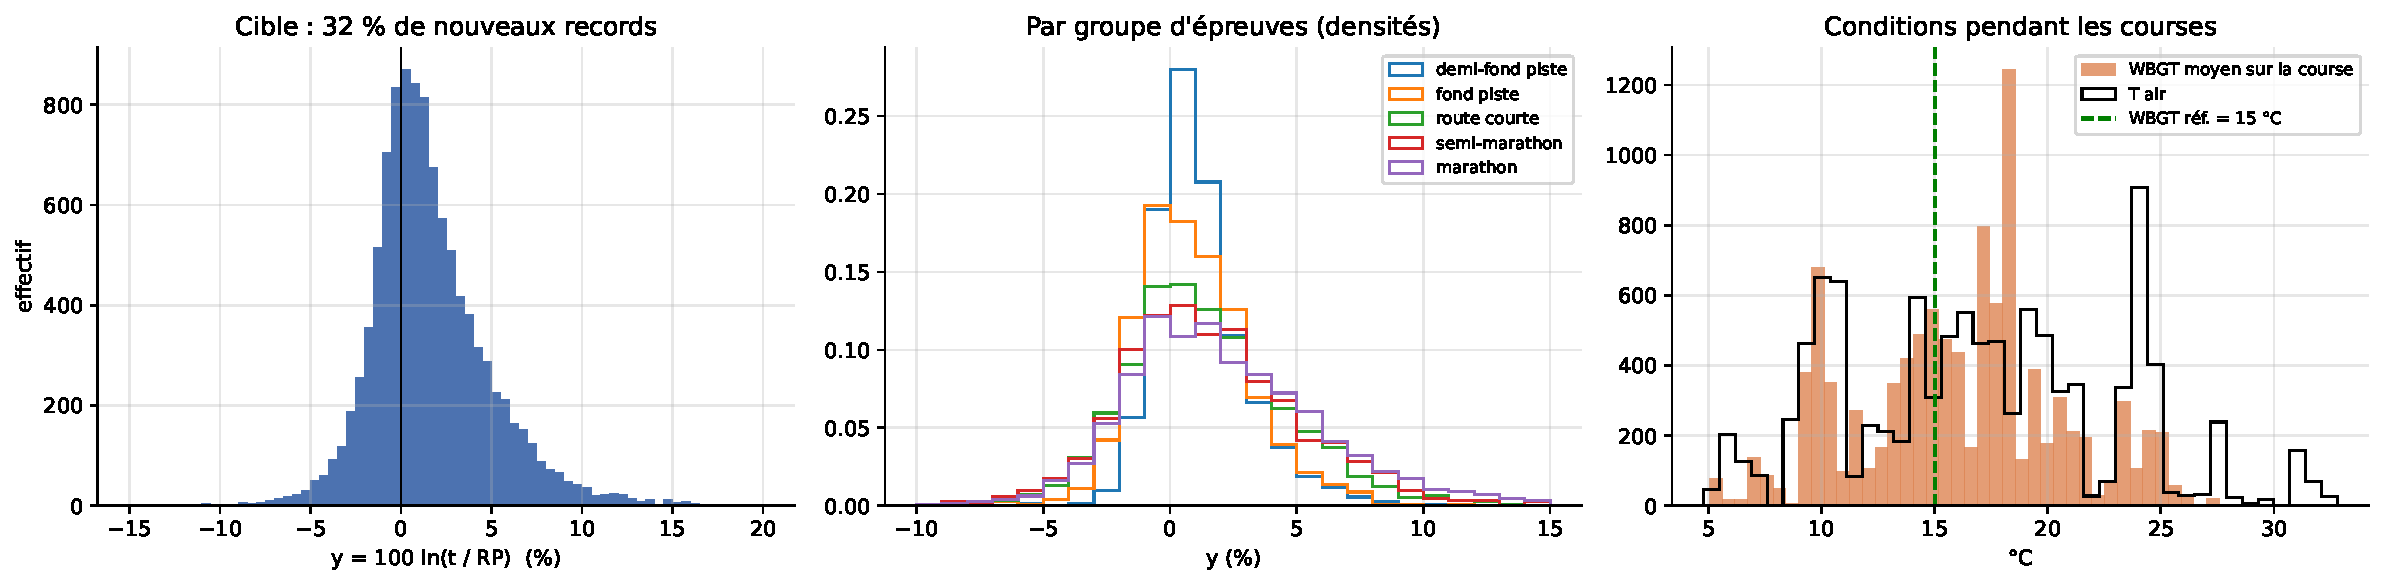
\includegraphics[width=\textwidth]{distributions}
\caption{À gauche, distribution de la cible $y$ sur les 10\,398 performances de l'échantillon d'analyse ; au centre,
densités de $y$ par groupe d'épreuves ; à droite, distributions du WBGT moyen sur la course et de la température de
l'air, avec le WBGT de référence de 15~°C.}
\label{fig:distributions}
\end{figure}

\paragraph{La forme de la cible.} Sur les 10\,398 performances, 32~\% sont plus rapides que le record d'avant course
(figure~\ref{fig:distributions}). La médiane vaut 1,1~\%, la moyenne 1,6~\%, et les centiles 5 et 95 sont à
$-2{,}8$~\% et $+7{,}5$~\%. La distribution est asymétrique à droite (coefficient d'asymétrie 0,87) et à queues
épaisses (kurtosis en excès 2,5) : 13,5~\% des performances sont à plus de 5~\% au-dessus du record, contre 1,2~\%
à plus de 5~\% en dessous. On peut courir bien plus lentement que son record, un jour sans, lors d'une course
tactique ou d'une blessure, ou simplement parce que le record date ; on court rarement beaucoup plus vite.

Que $y$ soit positif en moyenne est attendu et ne doit rien à la météo. Le record est le \emph{minimum} des
performances passées : une course quelconque est donc en moyenne plus lente que ce minimum, et l'écart est d'autant
plus grand que les performances d'un athlète sont dispersées. C'est ce qu'on observe : la moyenne croît avec la
dispersion, de 0,9 à 1,2~\% sur piste à 2,2~\% au marathon. Les 32~\% de records viennent surtout d'athlètes en
progression, jeunes ou dont le record est ancien ou établi sur peu de courses.

La dispersion croît avec la distance : l'écart-type de $y$ vaut 1,9~point en demi-fond, 2,2 en fond sur piste, 3,3 à
3,6 sur route et 4,0 au marathon, soit une variance quatre fois plus grande au marathon qu'en demi-fond. Les données
sont donc fortement \emph{hétéroscédastiques}. Le demi-fond est aussi le groupe le plus concentré autour de 0 et le
plus asymétrique (1,52) : les coureurs de 800 à 1\,500~m courent souvent, leur record est récent et proche de leur
niveau du moment, et seuls les mauvais jours les en éloignent. À l'inverse, 21~\% des marathoniens finissent à plus de
5~\% de leur record. Nous en avons tiré deux conséquences : une perte quadratique sera dominée par les erreurs sur
route et au marathon, si bien que les métriques devront être lues par groupe d'épreuves et pas seulement globalement ;
et les queues épaisses rendent l'erreur quadratique sensible à quelques contre-performances extrêmes, ce qui fait de
l'erreur absolue un complément utile. L'écart entre sexes est faible (moyenne 1,7~\% chez les femmes et 1,6~\% chez
les hommes, écarts-types 3,5 et 3,2) et s'explique en partie par la répartition entre épreuves.

\paragraph{Les conditions couvertes.} Le WBGT moyen sur la course va de 5 à 27,6~°C, avec une médiane de 16,4~°C.
Selon les seuils de l'ACSM, 12~\% des performances ont lieu sous 10~°C, 53~\% entre 10 et 18~°C, 26~\% entre 18 et
23~°C, 9~\% entre 23 et 28~°C, et aucune au-delà de 28~°C. Les plages diffèrent beaucoup selon le groupe. Le demi-fond
et le fond sur piste, courus lors de réunions d'été en soirée, vers 20~h, ne descendent jamais sous 13,5~°C, avec une
médiane de 18,3~°C en demi-fond. Le semi-marathon et le marathon, courus entre 8~h~30 et 10~h et en saison
intermédiaire, vont de 5 à 22~°C et de 6 à 26~°C, avec des médianes de 10,3 et 14,2~°C.

\paragraph{La météo est une variable de course.} Le WBGT varie très peu entre les coureurs d'une même course : l'écart
entre le premier et le dernier listé ne dépasse jamais 1,2~°C, avec une médiane de 0,24~°C au marathon. C'est encore
un effet de la troncature : les listes ne gardent que des coureurs rapides, arrivés à quelques minutes d'écart.
L'information disponible sur l'effet de la météo repose donc sur 396 courses, et non sur 10\,398 lignes. Ces courses
ont de plus des tailles très inégales : 14 performances en médiane, 293 au maximum (10~km de Lille), et les 20 plus
grosses courses représentent 32~\% des lignes. Or ces grosses courses (marathons de Valencia, Tokyo ou Berlin, semi de
Boulogne) se courent au frais, et les courses chaudes sont plus petites : 19~\% des courses ont un WBGT supérieur à
23~°C, contre 9~\% des performances. Une régression ordinaire, qui pondère chaque ligne de la même façon, donnerait
donc beaucoup de poids à quelques marathons frais et peu aux courses chaudes. Cette observation sera au cœur du
protocole de validation (section~\ref{sec:validation}) et des modèles mixtes (section~\ref{sec:mixtes}).

\paragraph{La composition du WBGT.} Le WBGT n'a pas la même composition selon le groupe d'épreuves. Sur piste, les
réunions du soir combinent un air chaud (température médiane de 23,8~°C en demi-fond), sec (humidité relative de
52~\%) et un soleil bas (190~W/m²). Les marathons du matin combinent un air plus frais (13,2~°C), plus humide (64~\%)
et un fort rayonnement (430~W/m²). Deux exemples extrêmes atteignent le même WBGT par des chemins opposés : le meeting
de Dessau 2026 (31,5~°C, humidité de 38~\%, 200~W/m², WBGT de 26,0~°C) et le marathon de Guiyang 2026 (21,2~°C
seulement, mais 73~\% d'humidité et 540~W/m², WBGT de 25,8~°C). Un modèle qui ne verrait que la température de l'air
classerait mal ces deux courses. À l'inverse, il n'est pas acquis qu'un même WBGT ait le même effet physiologique
quelle que soit sa composition ; la section~\ref{sec:meteo_brute} confronte le WBGT aux variables météorologiques
brutes.

La \emph{dérive pendant la course} est importante sur les longues distances : du départ au maximum, le WBGT monte en
médiane de 2,4~°C sur semi-marathon et de 3,7~°C au marathon, alors qu'elle est nulle sur piste. Le WBGT au départ,
seule valeur souvent publiée, sous-estime donc la contrainte subie, ce qui justifie a posteriori l'usage du WBGT moyen
sur la durée de course.

\begin{figure}[htbp]
\centering
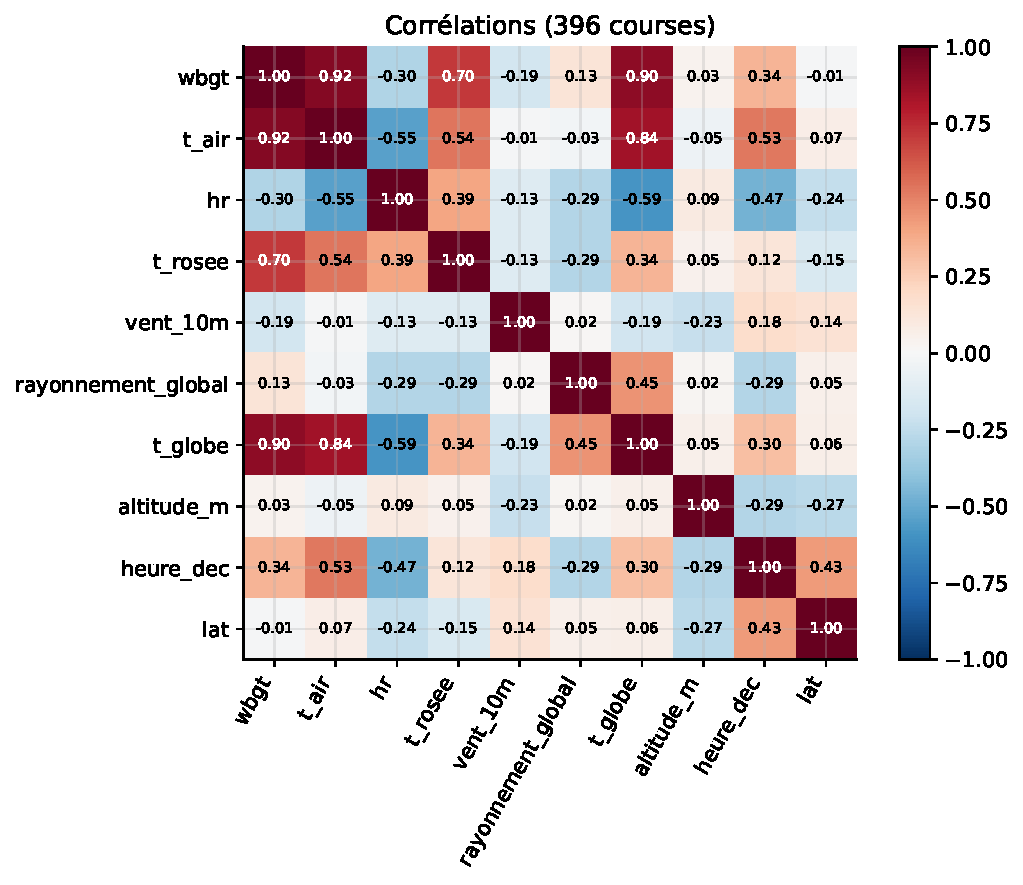
\includegraphics[width=0.56\textwidth]{correlations}
\caption{Corrélations de Pearson entre variables météorologiques et de contexte, calculées sur une ligne par course
(396 courses).}
\label{fig:correlations}
\end{figure}

\paragraph{Les corrélations entre variables météorologiques.} Les conditions étant communes à tous les coureurs d'une
course, nous calculons leurs corrélations sur une ligne par course : sans cela, une course de 293 coureurs compterait
293 fois. Le coefficient de corrélation de Pearson entre deux variables $u$ et $v$,
\[
r = \frac{\sum_c (u_c - \bar u)(v_c - \bar v)}{\sqrt{\sum_c (u_c - \bar u)^2}\,\sqrt{\sum_c (v_c - \bar v)^2}}
\in [-1\,;\,1],
\]
mesure la force d'une relation linéaire ; $r = 0$ n'exclut pas une relation non linéaire. Le WBGT est très corrélé à
la température de l'air (0,92) et à celle du globe (0,90), plus modérément au point de rosée (0,70), et peu au
rayonnement global pris seul (0,13), car les courses les plus chaudes sont les réunions du soir, sans soleil
(figure~\ref{fig:correlations}). L'humidité relative est anticorrélée à la température ($-0{,}55$) : c'est le cycle
diurne, au cours duquel l'humidité relative baisse quand l'air se réchauffe. Les combinaisons « chaud et humide » sont
donc rares, et il sera difficile de séparer les effets de la température et de l'humidité à partir des seules
données. C'est l'un des intérêts du WBGT : il combine ces grandeurs par un modèle physique, au lieu de demander au
modèle statistique d'apprendre cette combinaison. L'heure de départ est liée à la température (0,53) et à la latitude
(0,43) : elle encode surtout le type de réunion (piste le soir en Europe du Nord, route le matin) et sera un facteur
confondant à contrôler avec le groupe d'épreuves. L'altitude n'est presque pas corrélée au WBGT (0,03), ce qui permet
en principe d'estimer son effet séparément ; la pression, quasi déterminée par l'altitude, n'apporte rien de plus. Les
villes extrêmes illustrent d'ailleurs la saison plus que le climat : Houston (marathon et semi de janvier, 5,9~°C),
Buenos Aires (semi d'août, en hiver austral, 6,9~°C) ou Cape Elizabeth (10~km d'août, 26,5~°C). Avec une ou deux
courses par ville, ces moyennes ne caractérisent pas le climat local.

\paragraph{Les combinaisons mal représentées.} Plusieurs situations sont rares ou absentes : la piste au frais (moins
de 16~°C), le semi-marathon au chaud (aucune course au-delà de 22~°C), le marathon très chaud (8 courses seulement
au-dessus de 23~°C, soit 102 performances) et toute condition extrême (WBGT supérieur à 28~°C). Le croisement entre
épreuve et chaleur est défavorable : la moitié des courses au-dessus de 23~°C sont des courses de demi-fond, là où
l'effet attendu de la chaleur est le plus faible. Pour les longues distances, où l'effet est le plus fort,
l'information sur la chaleur est rare, et l'effet au marathon par forte chaleur reposera sur peu de courses. Les
autres facteurs sont peu variés. La pluie ne concerne que 37 courses (plus de 0,1~mm/h), et le vent à 10~m ne dépasse
pas 6,3~m/s. L'altitude n'est observée que sur route, dans 18 courses (168 performances, 1,6~\% des données) et 8 lieux
au-dessus de 1\,000~m, dont certains sont aussi chauds (Guiyang, Kigali, Lanzhou) : son effet sera difficile à séparer
de celui de la chaleur et du plateau.

Trois conséquences pour la modélisation se dégagent de cette description. Le groupe d'épreuves, ou la durée de course,
doit entrer dans le modèle en interaction avec le WBGT, puisque les plages de WBGT, le niveau moyen de $y$ et sa
dispersion diffèrent tous selon le groupe. La météo étant une variable de course, l'unité d'information est la course,
ce qui impose une validation groupée et une structure d'effets de course ou de parcours. Enfin, le domaine de validité
d'un outil fondé sur ces données est un WBGT de 5 à 27~°C, sans altitude marquée ni pluie forte ; au-delà, il faudra
signaler l'extrapolation à l'utilisateur.

\subsection{Une première relation brute, et le paradoxe de Simpson}\label{sec:simpson}

La première idée, pour avoir une idée de l'effet du WBGT, est de tracer la moyenne de $y$ par classe de WBGT. Nous
découpons le WBGT en classes de 3~°C. Dans la classe $b$, qui compte $n_b$ performances, nous calculons la moyenne
$\bar y_b$ et son \emph{erreur type}
\[
\mathrm{se}(\bar y_b) = \frac{s_b}{\sqrt{n_b}}, \qquad s_b^2 = \frac{1}{n_b - 1}\sum_{i \in b}(y_i - \bar y_b)^2 .
\]
L'erreur type est l'écart-type de l'\emph{estimateur} $\bar y_b$, c'est-à-dire sa variabilité d'un échantillon à
l'autre ; il ne faut pas la confondre avec l'écart-type $s_b$ des observations. Le diviseur $n_b - 1$ rend $s_b^2$
sans biais, la moyenne ayant été estimée sur les mêmes données. D'après le théorème central limite, $\bar y_b$ suit
approximativement une loi normale, d'où l'intervalle de confiance à 95~\% $\bar y_b \pm 1{,}96\,\mathrm{se}(\bar y_b)$,
où $1{,}96$ est le quantile d'ordre $0{,}975$ de la loi normale centrée réduite. Ces barres d'erreur reposent sur une
hypothèse cachée : la formule $\Var(\bar y_b) = \sigma^2/n_b$ suppose des observations indépendantes. Les coureurs
d'une même course partageant la météo et le déroulement de la course, ces barres sont trop étroites ; nous le
mesurerons en section~\ref{sec:dependance}.

Une seconde difficulté tient à la composition des classes. La moyenne de toutes les épreuves dans la classe $b$ est
une moyenne pondérée des moyennes de chaque groupe d'épreuves $e$ :
\[
\bar y_b = \sum_e \pi_{e \mid b}\,\bar y_{e, b},
\]
où $\pi_{e \mid b}$ est la part du groupe $e$ dans la classe $b$. Si cette composition change d'une classe à l'autre,
par exemple beaucoup de demi-fond dans les classes chaudes et beaucoup de marathons dans les classes fraîches, la
courbe globale peut monter, descendre ou s'aplatir alors même que chaque groupe présente une relation nette. Une
tendance agrégée peut ainsi différer, voire s'inverser, par rapport aux tendances de chaque sous-groupe : c'est le
\emph{paradoxe de Simpson}. D'où l'intérêt de lire les courbes par groupe d'épreuves.

\begin{figure}[htbp]
\centering
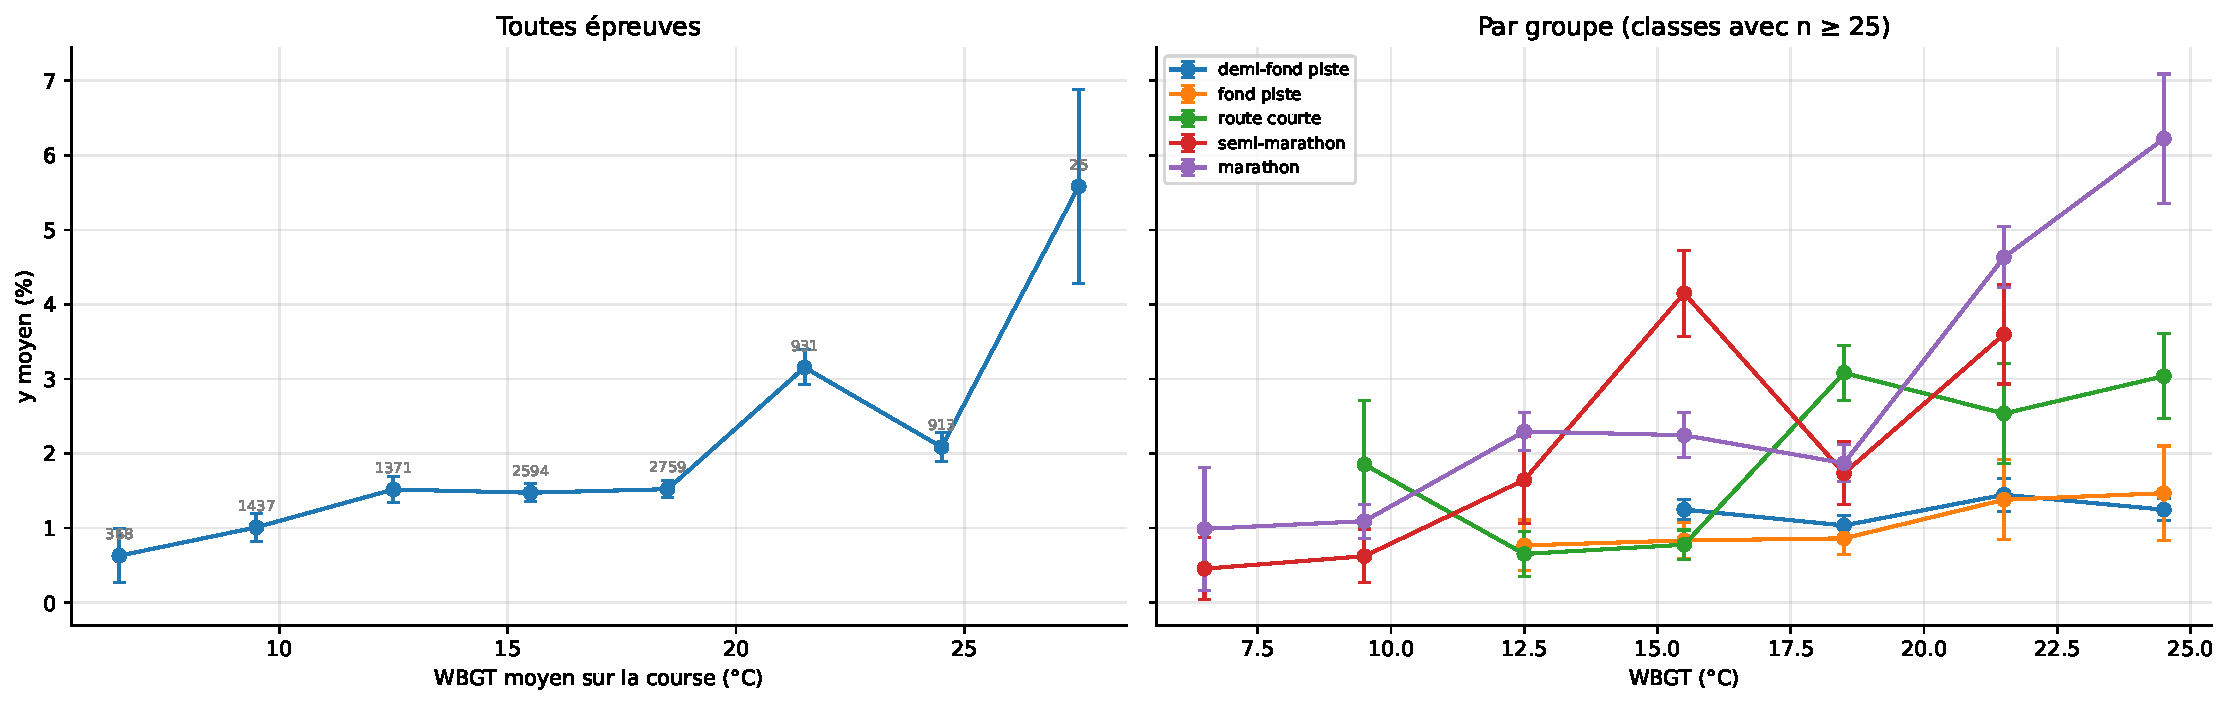
\includegraphics[width=\textwidth]{moyennes_classes}
\caption{Moyenne de $y$ par classe de WBGT de 3~°C, avec intervalles de confiance à 95~\% calculés sous hypothèse
d'indépendance. À gauche, toutes épreuves confondues (effectifs indiqués au-dessus des points) ; à droite, par groupe
d'épreuves, pour les classes d'au moins 25 performances.}
\label{fig:moyennes_classes}
\end{figure}

La figure~\ref{fig:moyennes_classes} illustre exactement ce phénomène. Toutes épreuves confondues, $\bar y$ monte de
0,6~\% (WBGT de 5 à 8~°C) à 1,0~\% (8 à 11~°C), reste vers 1,5~\% entre 11 et 20~°C, puis passe à 3,2~\% entre 20
et 23~°C. Il \emph{retombe} ensuite à 2,1~\% entre 23 et 26~°C, une classe composée à 69~\% de demi-fond sur piste,
avant d'atteindre 5,6~\% au-delà de 26~°C, sur 25 performances seulement. Par groupe, le contraste est net. Au
marathon, $\bar y$ vaut environ 1~\% jusqu'à 11~°C, 1,9 à 2,3~\% entre 11 et 20~°C, puis 4,6~\% entre 20 et 23~°C et
6,2~\% entre 23 et 26~°C : le ralentissement est fort et convexe, cohérent avec \citet{ely2007}. Le demi-fond et le
fond sur piste sont presque plats (0,8 à 1,5~\%) sur toute leur plage, de 12 à 26~°C. La route courte et le
semi-marathon présentent des profils irréguliers, comme le pic du semi-marathon entre 14 et 17~°C (4,2~\%) ; mais
chaque classe n'y réunit qu'une poignée de courses (2 à 20), et ces moyennes mélangent l'effet de la chaleur et celui
du lieu. La moyenne globale est donc trompeuse : sa forme dépend surtout du groupe d'épreuves qui domine chaque
classe.

\subsection{Les facteurs confondants}\label{sec:confondants}

Le WBGT n'est pas distribué au hasard. Les courses chaudes ont lieu dans certains pays (Asie du Sud-Est, Afrique de
l'Ouest, Golfe) et à certaines saisons, avec des plateaux différents en niveau, en âge et en proportion d'athlètes
établissant un record ; l'altitude se concentre dans quelques villes. D'après \eqref{eq:biais_omise}, un facteur
confondant n'est dangereux que s'il est lié au WBGT. Nous avons donc mesuré, au niveau des courses, la corrélation
entre le WBGT et chaque variable de contexte. Chaque course $c$ reçoit un poids $w_c = n_c/\sum_{c'} n_{c'}$
proportionnel à son nombre de coureurs, pour refléter son poids dans les données individuelles, et la corrélation
pondérée s'écrit
\[
r_w = \frac{\sum_c w_c\,(u_c - \bar u_w)(v_c - \bar v_w)}{\sqrt{\sum_c w_c\,(u_c - \bar u_w)^2}\,
\sqrt{\sum_c w_c\,(v_c - \bar v_w)^2}}, \qquad \bar u_w = \sum_c w_c\,u_c .
\]

\begin{figure}[htbp]
\centering
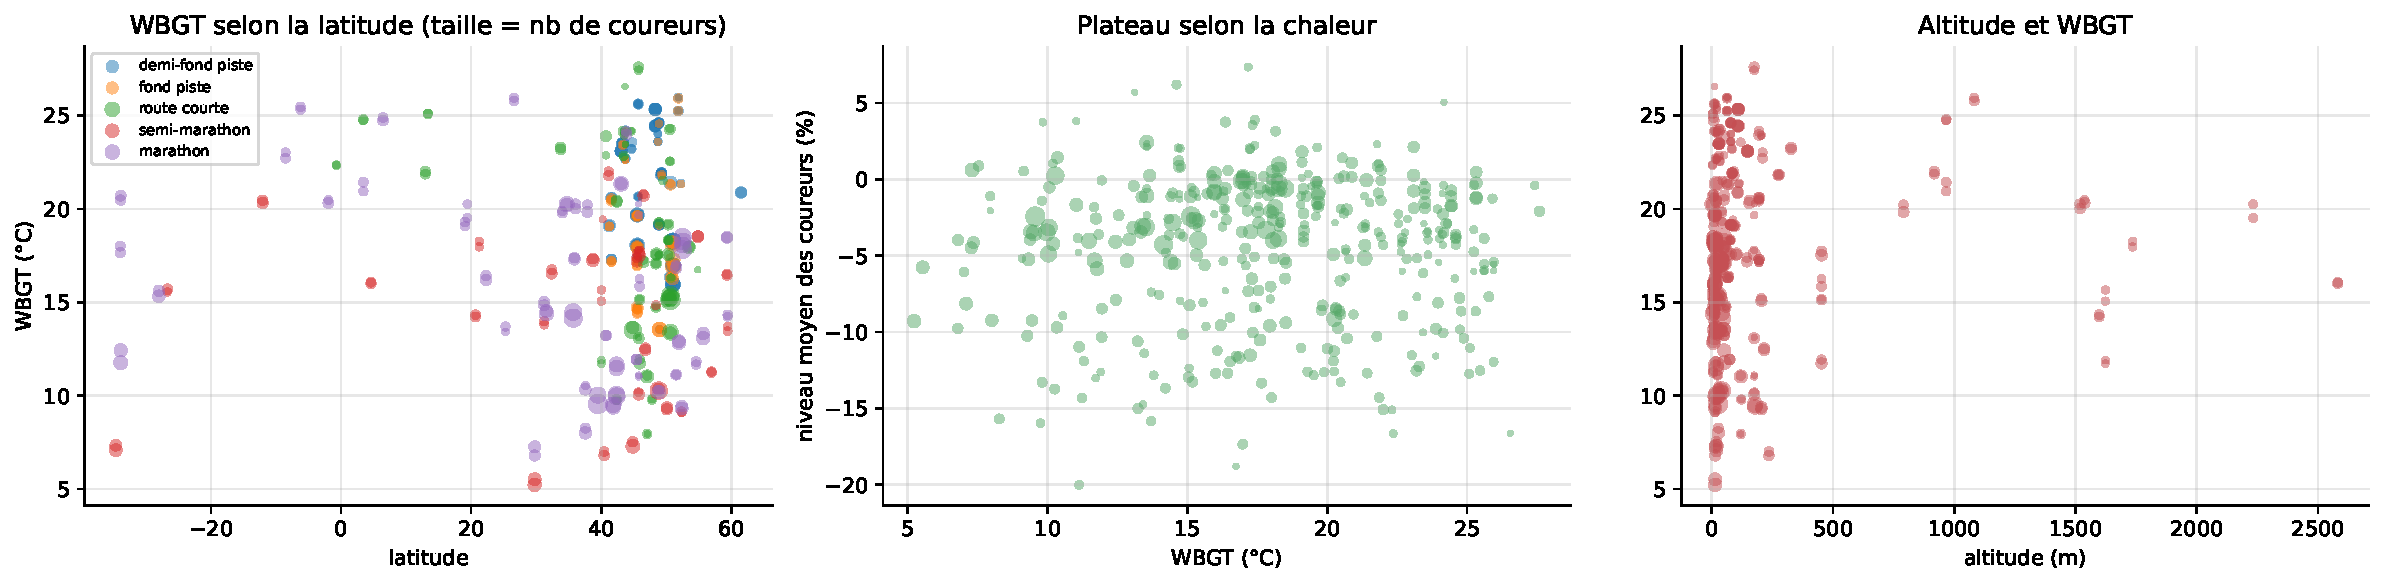
\includegraphics[width=\textwidth]{confusion}
\caption{Trois facteurs confondants potentiels, au niveau des courses (taille des points proportionnelle au nombre de
coureurs). À gauche, WBGT selon la latitude et le groupe d'épreuves ; au centre, niveau moyen des coureurs selon le
WBGT ; à droite, WBGT selon l'altitude.}
\label{fig:confusion}
\end{figure}

Au niveau des courses, le WBGT est corrélé à l'âge moyen des coureurs ($-0{,}43$), à l'heure de départ ($+0{,}42$),
à la forme ($-0{,}15$) et à l'altitude ($+0{,}13$), mais presque pas au niveau ($+0{,}05$, figure~\ref{fig:confusion}).
La formule \eqref{eq:biais_omise} permet alors d'anticiper le sens des biais d'une régression simple de $y$ sur le
WBGT. La composition des épreuves est le premier d'entre eux : les courses chaudes sont surtout des réunions de piste
(38 des 75 courses au-dessus de 23~°C sont du demi-fond), où la chaleur pèse peu, et les courses fraîches sont des
marathons et des semis ; l'effet moyen sous-estime donc celui du marathon et surestime celui du demi-fond. L'âge
ensuite : $y$ augmente fortement avec l'âge (0,7~\% avant 23~ans, 3,5 à 3,8~\% après 38~ans), car le record d'un
coureur âgé est ancien ; les courses chaudes réunissant des coureurs plus jeunes, $\beta_Z > 0$ et
$\Cov(W, Z) < 0$, et le biais est négatif. L'altitude joue en sens inverse : les lieux d'altitude (Kigali, Mexico,
Guiyang, Lanzhou) sont aussi chauds, et l'hypoxie ralentit, d'où un biais positif si l'altitude est omise. Le pays et
le parcours induisent un biais de sens inconnu : le WBGT est élevé sous les tropiques (Jakarta, Chon Buri, Lagos,
Cali) et lors des réunions d'été européennes, et ces courses diffèrent aussi par le profil, le plateau et l'enjeu.
Enfin, la sélection biaise vers le bas : par forte chaleur, des coureurs renoncent, abandonnent ou « gèrent », et la
troncature des listes coupe les performances lentes.

\subsection{La troncature : démonstration et remède}\label{sec:troncature}

Revenons sur le piège de la troncature, qui nous a longtemps occupés. Considérons deux coureurs de même niveau, dont
le record au marathon est de 2~h~30, dans une course qui ne liste que les hommes sous 2~h~37. Par temps frais, tous
deux finissent entre 2~h~30 et 2~h~35 : ils sont sous le seuil et apparaissent dans les résultats. Par fort WBGT, le
premier court en 2~h~36 et reste listé ; le second, davantage affecté par les conditions, court en 2~h~45, dépasse le
seuil et disparaît des résultats. Seul le coureur le plus résistant à la chaleur figure donc dans les données. Pour
les athlètes dont le record est proche du seuil, c'est-à-dire les moins rapides de la liste, on n'observe par forte
chaleur que ceux qui ont bien couru par rapport à leur niveau : leur ralentissement moyen est sous-estimé, et l'effet
de la chaleur est biaisé vers zéro.

Pour s'en convaincre, modélisons cette situation. Supposons qu'en l'absence de troncature,
$y_i = \mu_i + \varepsilon_i$ avec $\varepsilon_i \sim \mathcal{N}(0, \sigma^2)$, où $\mu_i = \E[y_i]$ est le
ralentissement moyen attendu pour l'athlète $i$ dans les conditions de sa course ; une hausse du WBGT augmente
$\mu_i$. On n'observe pourtant $y_i$ que si $y_i \leq m_i$, et la quantité réellement observée en moyenne est
$\E[y_i \mid y_i \leq m_i]$. Notons $\varphi$ et $\Phi$ la densité et la fonction de répartition de la loi normale
centrée réduite, et $a_i = (m_i - \mu_i)/\sigma$ la marge exprimée en écarts-types. Comme $z\varphi(z) =
-\varphi'(z)$,
\[
\E[\varepsilon \mid \varepsilon \leq \sigma a] = \frac{1}{\Phi(a)}\int_{-\infty}^a \sigma z\,\varphi(z)\,\dd z
= -\sigma\,\frac{\varphi(a)}{\Phi(a)},
\]
d'où l'espérance d'une loi normale tronquée par le haut :
\begin{equation}\label{eq:troncature}
\E[y_i \mid y_i \leq m_i] = \mu_i - \sigma\,\Lambda(a_i), \qquad \Lambda(a) = \frac{\varphi(a)}{\Phi(a)},
\end{equation}
où $\Lambda$ est l'inverse du ratio de Mills. Si la chaleur augmente $\mu_i$ de $\delta$, la moyenne observée
n'augmente donc que de $\delta\,\partial_\mu \E[y \mid y \leq m]$. Pour calculer cette dérivée, notons que
$a = (m - \mu)/\sigma$ dépend de $\mu$, avec $\partial a/\partial \mu = -1/\sigma$, et que, puisque
$\varphi'(a) = -a\,\varphi(a)$,
\[
\Lambda'(a) = \frac{\varphi'(a)\,\Phi(a) - \varphi(a)^2}{\Phi(a)^2} = -\Lambda(a)\big(a + \Lambda(a)\big).
\]
Il vient
\begin{equation}\label{eq:attenuation}
\frac{\partial}{\partial \mu}\big[\mu - \sigma\Lambda(a)\big] = 1 + \Lambda'(a) = 1 - \Lambda(a)\big(a + \Lambda(a)\big).
\end{equation}
Ce facteur est compris entre 0 et 1 : c'est aussi le rapport $\Var(y \mid y \leq m)/\sigma^2$, et la variance d'une
loi tronquée est toujours inférieure à celle de la loi complète. La pente estimée est donc \emph{atténuée}, d'autant
plus que la marge $a$ est faible. Quand la marge est grande, la troncature devient négligeable : $\Lambda(a) \to 0$,
le facteur tend vers 1 et le biais disparaît.

Cette analyse suggère directement le remède : ne garder que les athlètes dont la marge au seuil est suffisante,
$m_i \geq M$ pour une marge minimale $M$ fixée. Pour eux, tout ralentissement jusqu'à $M$~\% reste observable. Il est
essentiel que ce filtre porte sur le \emph{record} de l'athlète comparé au dernier temps listé, et non sur son
résultat du jour : il écarte les athlètes proches du seuil, pas ceux qui ont mal couru, et ne crée donc pas lui-même
de sélection sur $y$. Son coût est celui d'un échantillon plus petit et de meilleur niveau. Il réduit le biais sans
l'éliminer : un ralentissement supérieur à la marge, ou un abandon, reste invisible.

Les données confirment le mécanisme. Parmi les 4\,425 performances valides dont la marge est inférieure à 5~\%, 63~\%
sont des records personnels, contre 32~\% dans l'échantillon d'analyse : un athlète dont le record est proche du
dernier temps listé n'apparaît que s'il court vite.

Pour mesurer l'effet du choix de $M$, nous avons comparé la pente de $y$ en fonction du WBGT pour plusieurs marges
minimales (0, 2, 5, 8, 10 et 12~\%). Si la troncature biaise vers zéro, la pente doit augmenter avec $M$. L'outil est
la régression linéaire simple $y = \beta_0 + \beta_1 W + \varepsilon$, où $\beta_1$ est la pente en points de $y$
par degré, et $\varepsilon$ un aléa de moyenne nulle et de variance $\sigma^2$. Les moindres carrés retiennent les
valeurs de $(\beta_0, \beta_1)$ qui minimisent $S(\beta_0, \beta_1) = \sum_i (y_i - \beta_0 - \beta_1 W_i)^2$. La
condition $\partial S/\partial \beta_0 = 0$ donne $\hat\beta_0 = \bar y - \hat\beta_1\,\bar W$ : la droite passe par
le point moyen. La condition $\partial S/\partial \beta_1 = 0$ donne alors
$\sum_i (W_i - \bar W)(y_i - \bar y) = \hat\beta_1\sum_i (W_i - \bar W)^2$, d'où
\[
\hat\beta_1 = \frac{\sum_i (W_i - \bar W)(y_i - \bar y)}{\sum_i (W_i - \bar W)^2}
= \frac{\widehat{\Cov}(W, y)}{\widehat{\Var}(W)} = r\,\frac{s_y}{s_W} .
\]
La pente combine la force du lien linéaire $r$ et le rapport des échelles des deux variables. Puisque
$\sum_i (W_i - \bar W) = 0$, on peut écrire $\hat\beta_1 = S_{WW}^{-1}\sum_i (W_i - \bar W)\,y_i$ avec
$S_{WW} = \sum_i (W_i - \bar W)^2$ : c'est une combinaison linéaire des $y_i$. Avec des aléas indépendants de
variance $\sigma^2$,
\[
\E[\hat\beta_1] = \beta_1, \qquad \Var(\hat\beta_1) = \frac{\sigma^2}{S_{WW}}, \qquad
\widehat{\mathrm{se}}(\hat\beta_1) = \frac{\hat\sigma}{\sqrt{S_{WW}}} .
\]
L'erreur type diminue quand les données sont plus nombreuses, quand le WBGT varie sur une plage plus large et quand
le bruit est plus faible. Reste à estimer $\sigma^2$, à partir des résidus $\hat\varepsilon_i = y_i - \hat\beta_0 -
\hat\beta_1 W_i$. Ceux-ci vérifient deux contraintes, $\sum_i \hat\varepsilon_i = 0$ et
$\sum_i W_i\,\hat\varepsilon_i = 0$, et ne varient librement que dans un espace de dimension $n - 2$, le nombre de
\emph{degrés de liberté}. On montre que $\E\big[\sum_i \hat\varepsilon_i^2\big] = (n - 2)\,\sigma^2$, d'où
l'estimateur sans biais $\hat\sigma^2 = \sum_i \hat\varepsilon_i^2/(n - 2)$ ; diviser par $n$ sous-estimerait
$\sigma^2$, la droite étant ajustée au plus près des points. Pour $n$ grand, $\hat\beta_1$ est approximativement
normal, d'où l'intervalle de confiance à 95~\% $\hat\beta_1 \pm 1{,}96\,\widehat{\mathrm{se}}(\hat\beta_1)$.

\begin{figure}[htbp]
\centering
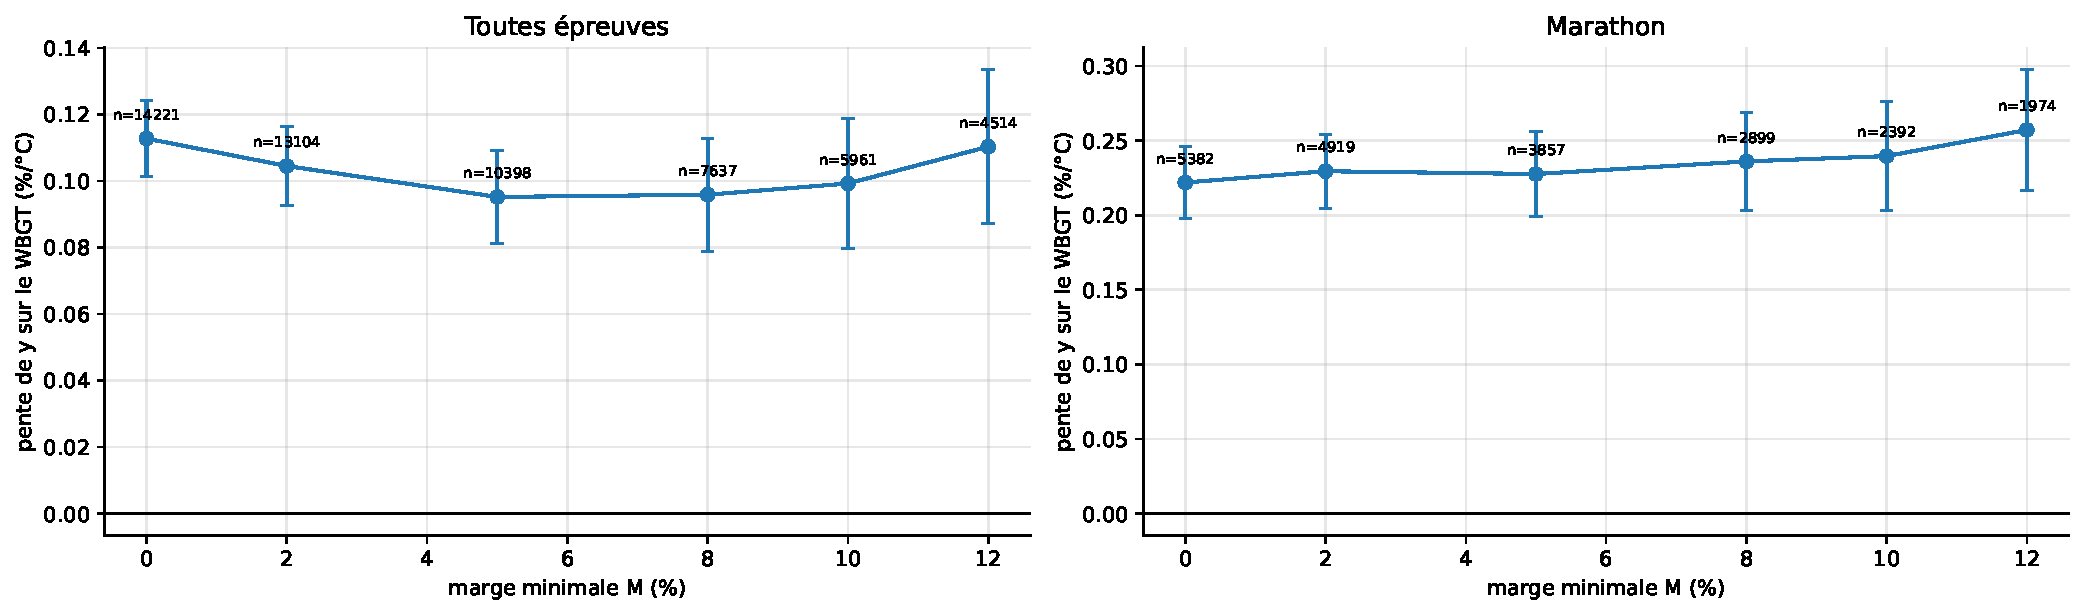
\includegraphics[width=\textwidth]{pentes_marge}
\caption{Pente de la régression simple de $y$ sur le WBGT selon la marge minimale $M$ exigée, toutes épreuves
confondues (à gauche) et au marathon (à droite), avec intervalles de confiance à 95~\% calculés sous hypothèse
d'indépendance. Les effectifs sont indiqués au-dessus des points.}
\label{fig:pentes_marge}
\end{figure}

Trois points guident la lecture de l'expérience. Sans troncature, la pente serait à peu près constante : le
sous-échantillon change, pas la vraie pente. Un $M$ plus grand réduit le biais mais retire des données, si bien que
l'intervalle de confiance s'élargit ; c'est un compromis entre biais et variance, et l'échantillon change aussi de
nature, puisqu'il ne garde que des athlètes plus rapides. Enfin, les sous-échantillons sont emboîtés (celui de
$M = 12$ est inclus dans celui de $M = 5$) : les pentes sont très corrélées entre elles, et des intervalles qui se
chevauchent ne suffisent pas à conclure que deux pentes sont égales.

La pente globale bouge peu avec la marge (figure~\ref{fig:pentes_marge}) : 0,113~point par degré sans filtre
($M = 0$, 14\,221 performances), 0,095 pour $M = 5$ et 0,110 pour $M = 12$ (4\,514 performances). Au marathon, seul
pour éviter le paradoxe de Simpson, elle croît avec $M$ : 0,222, puis 0,228 et 0,257~point par degré. C'est le sens
attendu : exiger une marge plus grande retire les courses où l'atténuation est possible. L'ampleur reste modeste,
$+15$~\% entre $M = 0$ et $M = 12$, dans les marges d'incertitude, alors que l'échantillon est divisé par 2,7. Nous
avons retenu $M = 5$~\% comme compromis, et nous reviendrons sur ce choix en section~\ref{sec:discussion} avec le
modèle final. Deux réserves s'imposent : la pente globale mêle les épreuves, et les intervalles affichés supposent des
performances indépendantes. La section suivante montre qu'ils sont en réalité environ deux fois trop étroits.

\subsection{Une structure de dépendance forte}\label{sec:dependance}

Les coureurs d'une même course partagent la météo, le déroulement de la course (lièvres, tactique) et le plateau ; les
éditions d'un même parcours partagent son profil. Nous avons voulu mesurer la part de la variance de $y$ commune aux
coureurs d'une même course, d'un même meeting, d'un même parcours ou d'un même lieu. L'outil naturel est la
\emph{corrélation intra-classe}.

Supposons les observations réparties en $G$ groupes et écrivons, pour l'athlète $j$ du groupe $g$,
\begin{equation}\label{eq:effet_aleatoire}
y_{gj} = \mu + u_g + \varepsilon_{gj}, \qquad u_g \sim \mathcal{N}(0, \tau^2), \qquad
\varepsilon_{gj} \sim \mathcal{N}(0, \sigma^2),
\end{equation}
tous indépendants. L'effet $u_g$ est partagé par toutes les observations du groupe (même météo, même train de course,
même parcours) ; $\varepsilon_{gj}$ est la part propre à l'individu. Deux coureurs d'un même groupe partagent le même
$u_g$, d'où
\[
\Var(y_{gj}) = \tau^2 + \sigma^2, \qquad \Cov(y_{gj}, y_{gj'}) = \Var(u_g) = \tau^2 \quad (j \neq j'), \qquad
\mathrm{ICC} = \Corr(y_{gj}, y_{gj'}) = \frac{\tau^2}{\tau^2 + \sigma^2} .
\]
L'ICC a deux lectures équivalentes : la part de la variance totale due aux groupes, et la corrélation entre deux
observations d'un même groupe. Elle est nulle si les groupes ne jouent aucun rôle, et vaut 1 si toutes les
observations d'un même groupe sont identiques.

Pour l'estimer avec des groupes de tailles inégales, nous utilisons l'estimateur de l'analyse de la variance. Avec
$N$ observations, $n_g$ observations dans le groupe $g$, $\bar y_g$ la moyenne du groupe et $\bar y$ la moyenne
générale, la variation totale se décompose en une part entre groupes et une part intra-groupes :
\[
\underbrace{\sum_g\sum_j(y_{gj}-\bar y)^2}_{\text{totale}}
= \underbrace{\sum_g n_g(\bar y_g-\bar y)^2}_{\text{entre groupes}}
+ \underbrace{\sum_g\sum_j(y_{gj}-\bar y_g)^2}_{\text{intra-groupes}} .
\]
Divisant chaque somme par son nombre de degrés de liberté, on définit les carrés moyens et une taille de groupe
effective $n_0$ :
\[
\mathrm{MSB} = \frac{\sum_g n_g(\bar y_g - \bar y)^2}{G-1},\qquad
\mathrm{MSW} = \frac{\sum_g\sum_j (y_{gj} - \bar y_g)^2}{N-G},\qquad
n_0 = \frac{N - \sum_g n_g^2/N}{G-1} .
\]
Sous le modèle \eqref{eq:effet_aleatoire}, $\E[\mathrm{MSW}] = \sigma^2$ et $\E[\mathrm{MSB}] = \sigma^2 + n_0\,\tau^2$.
Au sein d'un groupe, en effet, $u_g$ est commun à tous et disparaît des écarts $y_{gj} - \bar y_g$, qui ne contiennent
que le bruit individuel ; il reste $N - G$ degrés de liberté, puisque $G$ moyennes ont été estimées. Les moyennes de
groupe varient au contraire pour deux raisons : les vraies différences entre groupes, de variance $\tau^2$, et le
bruit d'échantillonnage, de variance $\sigma^2/n_g$. En développant l'espérance de la somme entre groupes, on obtient
$(G - 1)\,\sigma^2 + \big(N - \sum_g n_g^2/N\big)\,\tau^2$, d'où le facteur $n_0$. Si tous les groupes ont la même
taille $n$, $n_0 = n$ ; s'ils sont déséquilibrés, $n_0$ est inférieur à l'effectif moyen $N/G$, car les gros groupes
apportent moins d'information sur $\tau^2$ que leur taille ne le suggère. En égalant chaque carré moyen à son
espérance, on obtient l'estimateur des moments
\[
\hat\sigma^2 = \mathrm{MSW}, \qquad \hat\tau^2 = \frac{\mathrm{MSB}-\mathrm{MSW}}{n_0}, \qquad
\widehat{\mathrm{ICC}} = \frac{\mathrm{MSB} - \mathrm{MSW}}{\mathrm{MSB} + (n_0 - 1)\,\mathrm{MSW}} .
\]
Quand la vraie ICC est proche de 0, MSB peut être inférieur à MSW par hasard, et l'estimateur légèrement négatif ; nous
ne le tronquons pas à 0, ce qui introduirait un biais vers le haut.

La conséquence pratique de l'ICC se lit sur la variance d'une moyenne. Pour $n$ observations d'un même groupe,
corrélées deux à deux avec la corrélation $\rho$ et de variance $\sigma_t^2 = \tau^2 + \sigma^2$,
\[
\Var(\bar y) = \frac{1}{n^2}\Big[n\,\sigma_t^2 + n(n-1)\,\rho\,\sigma_t^2\Big] = \frac{\sigma_t^2}{n}\,
\big[1 + (n - 1)\rho\big].
\]
Le facteur $\mathrm{deff} = 1 + (\bar n - 1)\rho$, appelé \emph{effet de plan} \citep{kish1965}, mesure de combien la
corrélation multiplie la variance par rapport à des observations indépendantes. La \emph{taille d'échantillon
effective} $N/\mathrm{deff}$ est le nombre d'observations indépendantes qui apporteraient la même information.

Le résultat a été l'une des surprises de l'étude. Environ 17~\% de la variance de $y$ est commune aux coureurs d'une
même course (ICC de 0,18), d'un même meeting (0,17), d'un même parcours (0,17) ou d'un même lieu (0,16). Ces valeurs
sont presque égales : l'essentiel de ce qui est partagé l'est déjà au niveau du lieu (météo, parcours, plateau, chrono
du jour), et l'on ne gagne presque rien à descendre à la course. Avec en moyenne 26 performances par course, l'effet de
plan vaut environ $1 + 25 \times 0{,}18 \approx 5{,}5$ : les 10\,398 performances ne valent qu'environ 1\,900
observations indépendantes, et seulement 396 situations météorologiques distinctes. Quatre conséquences en découlent :
les intervalles de confiance calculés sous hypothèse d'indépendance sont environ $\sqrt{5{,}5} \approx 2{,}3$ fois trop
étroits ; des plis de validation aléatoires laisseraient fuiter les effets de lieu ; les intervalles de confiance
devront rééchantillonner des lieux, et non des lignes ; enfin, un modèle à effet aléatoire de course est naturel.

\section{Un protocole de validation à l'épreuve des fuites}\label{sec:validation}

L'outil final servira à estimer l'effet des conditions météorologiques dans une ville et une course qui n'ont jamais
été observées. Le protocole d'évaluation doit reproduire cette situation : un modèle n'est jugé que sur des données
absentes de son apprentissage, et ces données doivent en être aussi indépendantes que le seront celles d'un usage réel.
La structure de dépendance mise au jour en section~\ref{sec:dependance} rend cette exigence décisive.

\subsection{Fuites d'information et regroupement par lieu}\label{sec:fuites}

Notons $\ell$ une fonction de perte et $f$ un prédicteur. L'erreur mesurée sur un ensemble de validation n'estime sans
biais le risque de généralisation $\mathcal{R}(f) = \E[\ell(f(x), y)]$ que si les ensembles d'apprentissage et de
validation sont indépendants. Lorsqu'une information partagée entre les deux ensembles est disponible à l'évaluation
mais ne le sera pas lors de l'usage réel, l'erreur mesurée est trop optimiste : on parle de \emph{fuite
d'information}. Trois structures de dépendance sont en cause ici. La météo et les aléas sont d'abord partagés au sein
d'une course et d'un meeting : tous les coureurs d'une course subissent presque le même WBGT et le même déroulement
(lièvres, tactique, vent de face dans la dernière ligne droite). Un découpage aléatoire des lignes placerait une même
course des deux côtés, et le modèle pourrait associer l'aléa du jour à une valeur de WBGT et être récompensé pour ce
surapprentissage. La vitesse d'un parcours est ensuite partagée entre ses éditions : Boston reste vallonné d'une année
à l'autre, Valencia reste rapide. Si l'édition 2023 est en apprentissage et l'édition 2026 en validation, le modèle peut
reconnaître le parcours, par son altitude et ses conditions typiques, et en tirer profit sans avoir rien appris de
l'effet de la météo. Les athlètes, enfin, peuvent apparaître plusieurs fois ; c'est rare dans nos données, et leur
niveau est déjà absorbé par le record personnel.

Nous avons donc regroupé les données au niveau le plus englobant, le lieu : toutes les courses, éditions et épreuves
d'une même ville sont placées du même côté de chaque découpage. Ce choix prudent ne coûte presque rien, puisque l'ICC
de lieu (0,16) est proche de celle de la course (0,18).

Environ 20~\% des lieux sont d'abord mis de côté pour former l'\emph{ensemble de test}. Les conditions chaudes étant
rares, le tirage est stratifié : les lieux sont répartis en trois tiers de climat selon leur WBGT moyen, puis
$\lceil 0{,}2\, n_{\text{tiers}} \rceil$ lieux sont tirés au hasard dans chaque tiers, où $n_{\text{tiers}}$ est le
nombre de lieux du tiers. L'ensemble de test contient ainsi des lieux chauds, frais et intermédiaires. Il n'est
utilisé \emph{qu'une seule fois}, pour l'évaluation finale (section~\ref{sec:comparaison}) : choisir un modèle ou un
hyperparamètre sur le test rendrait son erreur optimiste.

Sur les lieux restants, les modèles et leurs hyperparamètres sont choisis par \emph{validation croisée} à $K = 5$
plis. Pour chaque pli $k$, un modèle est entraîné sur les quatre autres plis, notés $\mathcal{A}_k$, puis évalué sur
le pli $k$, noté $\mathcal{V}_k$ ; le risque est estimé par la moyenne des $K$ erreurs. Chaque pli est formé de lieux
entiers. Pour équilibrer les plis en nombre de performances, les lieux sont affectés de façon gloutonne : on les
ordonne par effectif décroissant, puis on place chacun dans le pli le moins rempli.

L'ensemble de test ainsi obtenu compte 21 lieux et 2\,355 performances (23~\% des données). Il couvre bien la plage
de climats, avec un WBGT moyen par lieu allant de 9,5~°C (marathon de Chicago) à 26,5~°C (Cape Elizabeth) : des lieux
frais (Chicago, Valencia, Auxerre, Cholet), intermédiaires (Annecy, Brest, Le Cap) et chauds (Ordizia, Smederevo, Chon
Buri, Jakarta). Deux lieux y pèsent lourd : Portland (686 performances de piste) et Valencia (415 performances de
marathon). Les 79 lieux restants (8\,043 performances) forment cinq plis équilibrés de 1\,607 à 1\,611 performances,
soit 14 à 17 lieux chacun. Aucun identifiant de lieu, de parcours, de meeting ou de course n'est commun à
l'apprentissage et à la validation. À titre de comparaison, un découpage aléatoire des lignes, à raison de 80~\% pour
l'apprentissage, partagerait 77 des 79 lieux, 119 parcours, 105 meetings et 247 courses entre apprentissage et
validation : presque toutes les structures de dépendance identifiées seraient présentes des deux côtés. La
section~\ref{sec:meteo_brute} mesurera le coût de cette fuite.

\subsection{Métriques d'évaluation}\label{sec:metriques}

Pour $n$ observations $y_i$ et leurs prédictions $\hat y_i$, nous utilisons trois métriques :
\[
\mathrm{RMSE} = \sqrt{\frac1n\sum_i (y_i - \hat y_i)^2},\qquad
\mathrm{MAE} = \frac1n\sum_i |y_i - \hat y_i|,\qquad
R^2 = 1 - \frac{\sum_i (y_i - \hat y_i)^2}{\sum_i (y_i - \bar y)^2}.
\]
La racine de l'erreur quadratique moyenne (RMSE) s'exprime dans l'unité de $y$, en points de pourcentage, et pénalise
fortement les grandes erreurs. Elle correspond à la perte quadratique, dont le minimiseur est l'espérance
conditionnelle $\E[y \mid x]$ : c'est notre métrique principale, cohérente avec la perte utilisée par les modèles.
L'erreur absolue moyenne (MAE) correspond à la perte absolue, dont le minimiseur est la médiane conditionnelle ; elle
est plus robuste aux valeurs extrêmes, et constitue un complément utile pour une cible asymétrique, à queues épaisses
et hétéroscédastique. Le coefficient $R^2$ mesure la part de la variance de $y$ expliquée par le modèle, par
comparaison avec la prédiction constante $\bar y$ calculée sur l'échantillon évalué. Hors échantillon, il peut être
négatif : le modèle fait alors moins bien que cette moyenne. Même le modèle constant obtient un $R^2$ de validation
légèrement négatif, puisqu'il prédit la moyenne de l'apprentissage et non celle du pli évalué.

Nous attendions des $R^2$ modestes. L'essentiel de la variance de $y$ vient de la variabilité d'une course à l'autre et
d'un coureur à l'autre (forme du jour, tactique, ancienneté du record), que la météo n'explique qu'en partie. Pour
l'outil final, la qualité de l'\emph{estimation de l'effet} de la chaleur, c'est-à-dire de la courbe de dégradation,
compte d'ailleurs autant que la précision des prédictions individuelles.

\subsection{Variables dérivées et décomposition de Mundlak}\label{sec:mundlak}

Trois variables ont été ajoutées. Elles sont calculées à l'intérieur d'une ligne ou d'un parcours ; un parcours
appartenant à un seul lieu, leur calcul n'introduit aucune fuite entre les plis. La première est le logarithme de la
durée de course attendue : l'effet de la chaleur croît avec la durée de l'effort, et le logarithme place sur une même
échelle un 800~m (environ deux minutes) et un marathon (environ 150 minutes). La deuxième est l'\emph{altitude utile}
$\max(0,\ \text{altitude} - 500)/1000$, en kilomètres au-delà de 500~m : cette fonction charnière traduit l'hypothèse
physiologique d'un effet de l'hypoxie négligeable sous 500~m et linéaire au-delà.

La troisième répond à la question des facteurs confondants entre lieux. Notons $\bar W_g$ le WBGT moyen du parcours
$g$, toutes éditions et tous coureurs confondus. Tout WBGT se décompose en
\begin{equation}\label{eq:mundlak}
W_{gj} = \underbrace{\bar W_g}_{\text{inter-parcours}} + \underbrace{(W_{gj} - \bar W_g)}_{\text{intra-parcours}} .
\end{equation}
La composante intra-parcours varie d'une édition à l'autre, ou entre coureurs rapides et lents d'une même course qui ne
courent pas pendant les mêmes heures : elle compare un parcours à lui-même, et reste à l'abri des différences entre
parcours. La composante inter-parcours compare au contraire des parcours différents et reste exposée aux facteurs
confondants de la section~\ref{sec:confondants}. Introduire $\bar W_g$ comme régresseur supplémentaire permet au
coefficient du WBGT de ne capter que l'effet intra-parcours \citep{mundlak1978} ; nous en verrons la justification
formelle en section~\ref{sec:quel_estimateur}.

Cette décomposition a révélé une limite sérieuse des données : l'écart-type du WBGT est de 4,52~°C sur l'ensemble des
données, mais de 1,04~°C seulement au sein d'un parcours. La variation intra-parcours ne représente donc qu'environ
5~\% de la variance du WBGT ($1{,}04^2/4{,}52^2 \approx 0{,}05$). L'essentiel de l'information sur la chaleur provient
de la comparaison entre lieux, exposée aux facteurs confondants ; une estimation fondée sur la seule variation
intra-parcours sera mieux protégée de ces biais, mais reposera sur une faible variation et devra être extrapolée pour
décrire un écart de 10~°C. Par ailleurs, l'altitude au-delà de 1\,000~m ne concerne que 168 performances, dans
8~lieux, et les valeurs manquantes se limitent à l'âge (9,2~\%) et à la forme (45,1~\%, faute de meilleure performance
de la saison d'avant course).

\subsection{Un prétraitement appris sur l'apprentissage seulement}\label{sec:pretraitement}

Les modèles opèrent sur une matrice numérique $X \in \mathbb{R}^{n \times p}$. Tous les paramètres du prétraitement
(médianes, moyennes, écarts-types, modalités) sont appris sur $\mathcal{A}_k$ seulement, puis appliqués tels quels à
$\mathcal{V}_k$ ou au test : les estimer sur l'ensemble des données constituerait une fuite, puisque le prétraitement
« connaîtrait » les lieux de validation. Les valeurs manquantes sont imputées par la médiane d'apprentissage, robuste
aux valeurs extrêmes, et une indicatrice de manquant est ajoutée, car l'absence d'une donnée peut être informative : un
athlète sans meilleure performance de la saison d'avant course n'a souvent pas couru l'épreuve plus tôt dans l'année.
Les variables sont enfin standardisées, $z = (x - \bar x)/s$. La standardisation est nécessaire à la pénalité ridge,
qui dépend de l'échelle des coefficients, et facilite l'optimisation des réseaux de neurones ; elle est inutile pour
les arbres, invariants par transformation monotone des variables.

Chaque modalité d'une variable catégorielle vue à l'apprentissage reçoit une colonne indicatrice (encodage
\emph{one-hot}) ; une modalité inconnue produit une ligne de zéros. Si toutes les modalités sont encodées et que le
modèle comporte une constante, la somme des indicatrices est égale à la colonne constante : $X$ n'est plus de rang
plein et $X^\top X$ n'est pas inversible. Lorsque c'est nécessaire, nous omettons donc une modalité dite de
référence, dont les autres coefficients mesurent l'écart. Appliqué aux variables de contexte, ce prétraitement produit
15 colonnes : 6 variables numériques, 2 indicatrices de manquant, 5 groupes d'épreuves et 2 sexes.

\subsection{La validation croisée et sa variabilité}\label{sec:cv}

La validation croisée est une procédure générique : pour chaque pli $k$, un modèle neuf est créé, de sorte qu'aucune
information ne passe d'un pli à l'autre, entraîné sur $\mathcal{A}_k$ puis évalué sur $\mathcal{V}_k$. La procédure
conserve aussi les \emph{prédictions hors pli} : chaque performance d'apprentissage reçoit la prédiction d'un modèle
qui ne l'a pas vue, ce qui permet d'analyser les erreurs sur l'ensemble des données d'apprentissage.

Le modèle constant, qui prédit la moyenne de $y$ sur l'apprentissage, fournit le premier point de référence. Sa RMSE
de validation croisée vaut 3,30 en moyenne, mais varie beaucoup d'un pli à l'autre : de 2,65 sur le pli~0 à 3,67 sur
le pli~1. L'écart-type entre plis (0,43) donne une erreur type de la moyenne d'environ $0{,}43/\sqrt5 \approx 0{,}19$.
Cette variabilité fixe l'échelle des comparaisons à venir : un écart de quelques centièmes de RMSE entre deux modèles
ne sera pas significatif. Comme les plis sont communs à tous les modèles, les comparaisons devront être faites pli par
pli, un pli difficile pesant sur tous les modèles à la fois. Les $R^2$ du modèle constant sont légèrement négatifs, de
$-0{,}017$ à $-0{,}0001$, comme attendu.

\section{Premiers modèles : régressions linéaires}\label{sec:lineaires}

Avant de recourir à des modèles flexibles, nous avons établi des points de référence simples. Ils répondent à deux
questions : quelle part de la variance de $y$ est prévisible sur un lieu nouveau, et quelle part de cette
prévisibilité revient à la météo plutôt qu'au profil des athlètes ? Ils fournissent aussi une première estimation de
l'effet de la chaleur, dont la section~\ref{sec:confondants} a montré qu'elle était exposée à plusieurs biais.

\subsection{Modèles naïfs}\label{sec:naifs}

Deux modèles sans aucune variable explicative servent de plancher. Le modèle constant prédit la moyenne de $y$ sur
l'apprentissage ; tout modèle utile doit faire mieux. Le modèle des moyennes par groupe prédit la moyenne de $y$ dans
la cellule épreuve $\times$ sexe de la performance, et la moyenne globale pour une cellule absente de l'apprentissage :
il teste si le seul niveau moyen de chaque groupe se transpose à des lieux nouveaux.

Le modèle constant obtient une RMSE de validation croisée de 3,300, et le modèle des moyennes par groupe 3,303 :
connaître l'épreuve et le sexe n'apporte rien en moyenne. Le détail par pli est instructif. Les moyennes par groupe
font mieux sur trois plis, jusqu'à $0{,}10$ de moins sur le pli~0, et moins bien sur les deux autres, jusqu'à $0{,}15$
de plus sur le pli~1. Les écarts de $y$ moyen entre groupes, de l'ordre d'un point, sont faibles devant la variabilité
d'un lieu à l'autre, et les moyennes apprises sur certains lieux ne se transposent pas aux autres : estimer dix
moyennes ajoute de la variance d'estimation sans information transposable.

\subsection{Moindres carrés ordinaires et régression ridge}\label{sec:ridge}

On ajoute à $X$ une colonne de 1, la constante, et l'on cherche les coefficients $w$ qui minimisent
$\mathcal{L}(w) = \lVert y - Xw\rVert^2$. Le gradient $\nabla\mathcal{L}(w) = -2X^\top(y - Xw)$ s'annule pour les
\emph{équations normales}
\[
X^\top X\,\hat w = X^\top y, \qquad \text{soit} \qquad \hat w = (X^\top X)^{-1}X^\top y
\quad \text{si } X^\top X \text{ est inversible.}
\]
Géométriquement, $X\hat w$ est la projection orthogonale de $y$ sur l'espace engendré par les colonnes de $X$, et le
résidu $y - X\hat w$ est orthogonal à chacune d'elles. Si des colonnes sont colinéaires, $X^\top X$ n'est pas
inversible et il existe une infinité de solutions ; nous retenons alors la solution de norme minimale
$\hat w = X^+ y$, où $X^+$ est la pseudo-inverse de Moore-Penrose, calculée par décomposition en valeurs singulières.

La régression ridge, ou régularisation de Tikhonov, ajoute à la perte une pénalité sur la taille des coefficients,
sans pénaliser la constante $b$ :
\[
\mathcal{L}(b, w) = \frac1n\sum_i (y_i - b - x_i^\top w)^2 + \lambda\lVert w\rVert^2 .
\]
La constante fixe le niveau moyen de $y$, qui n'a aucune raison d'être proche de 0 : la pénaliser biaiserait toutes
les prédictions. L'annulation de la dérivée en $b$ donne $\hat b = \bar y - \bar x^\top \hat w$. En reportant, le
problème ne porte plus que sur les données centrées $X_c = X - \mathbf{1}\bar x^\top$ et $y_c = y - \bar y\,\mathbf{1}$,
et l'annulation du gradient en $w$ conduit à
\[
\hat w = (X_c^\top X_c + n\lambda I)^{-1}X_c^\top y_c,\qquad \hat b = \bar y - \bar x^\top \hat w.
\]
La matrice $X_c^\top X_c + n\lambda I$ est définie positive dès que $\lambda > 0$ : la solution existe toujours, même
avec des colonnes colinéaires. L'effet de la pénalité se lit sur la décomposition en valeurs singulières
$X_c = UDV^\top$, de colonnes $u_j$ et de valeurs singulières $d_j$ : la prédiction s'écrit
\[
X_c\hat w = \sum_j u_j\, \frac{d_j^2}{d_j^2 + n\lambda}\, u_j^\top y_c .
\]
Chaque direction de l'espace des variables est rétrécie par le facteur $d_j^2/(d_j^2 + n\lambda) \in \,]0\,;\,1[$ :
les directions de faible variance, mal déterminées par les données et instables par moindres carrés, sont les plus
atténuées. Le ridge accepte un biais, des coefficients tirés vers 0, en échange d'une moindre variance. Deux
conséquences nous serviront : la pénalité dépend de l'échelle des variables, d'où la standardisation ; et, face à deux
variables presque colinéaires, le ridge tend à répartir l'effet entre elles, puisque pour une somme $w_1 + w_2$ donnée,
$w_1^2 + w_2^2$ est minimale quand $w_1 = w_2$.

\subsection{Une base polynomiale pour le WBGT}\label{sec:polynome}

La figure~\ref{fig:moyennes_classes} suggère une relation non linéaire entre WBGT et performance, au moins au
marathon. Pour la représenter dans un modèle linéaire en ses paramètres, nous remplaçons le WBGT $W$ par la base
polynomiale
\[
\psi(W) = \big(z, z^2, \dots, z^D\big), \qquad z = \frac{W - W_{\text{ref}}}{5},
\]
de degré $D$, où $5$~°C est une échelle fixée. Centrer et réduire avant d'élever à la puissance évite des colonnes
d'ordres de grandeur très différents ($25^3 \approx 15\,600$ contre $25$), qui rendraient $X^\top X$ mal conditionnée.
Le centre et l'échelle sont fixés a priori, car estimés sur les données ils changeraient d'un pli à l'autre ; la
puissance 0 est exclue, la constante étant gérée par le modèle. Les termes en WBGT peuvent en outre interagir avec le
groupe d'épreuves, ce qui permet à la courbe de différer d'un groupe à l'autre.

\subsection{Ce que les modèles linéaires nous ont appris}\label{sec:resultats_lineaires}

Nous avons comparé trois familles de modèles en validation croisée par lieux : les moindres carrés sur le WBGT seul,
qui reproduisent la régression simple de la section~\ref{sec:troncature} ; le ridge polynomial sur le WBGT seul, avec
un degré $D \in \{1, 2, 3, 4\}$ et $\lambda \in [10^{-3}\,;\,10]$ choisis par validation croisée ; et le ridge
complet, qui ajoute au WBGT (de degré $D \le 3$) les variables de contrôle (niveau, âge, forme, durée, altitude,
heure, vent, pluie, groupe d'épreuves, sexe), avec ou sans interactions entre WBGT et groupe d'épreuves, et avec ou
sans terme de Mundlak, soit 48 configurations.

Pour résumer l'effet de la chaleur selon un modèle $f$, nous utilisons l'effet moyen d'une hausse de 10~°C du WBGT
au-dessus de la référence,
\[
\overline{\Delta}_{10} = \frac1n \sum_i \Big[ f(x_i \mid W = W_{\text{ref}} + 10) - f(x_i \mid W = W_{\text{ref}}) \Big],
\]
toutes les autres variables gardant leurs valeurs observées. Pour un modèle linéaire de degré 1 sans interaction,
c'est exactement dix fois la pente du WBGT.

\paragraph{Le WBGT seul n'apporte presque rien en prédiction.} Les moindres carrés sur le WBGT obtiennent une RMSE de
3,301, légèrement moins bonne que celle du modèle constant (3,300). Le meilleur ridge polynomial ($D = 1$,
$\lambda = 1$) atteint 3,291, soit un gain de 0,009 seulement, et toute la grille tient entre 3,291 et 3,323. Les
degrés 2 à 4 ne font jeu égal avec le degré 1 qu'avec une pénalité forte, qui ramène le polynôme vers une droite :
rien ne justifie une courbure à ce stade. Ce résultat n'implique pas que la chaleur soit sans effet. La variance de
$y$ est dominée par les différences entre courses et entre coureurs, et l'effet brut du WBGT est brouillé par la
composition des épreuves et par les facteurs confondants ; un modèle qui ne voit que le WBGT ne peut pas séparer ces
contributions.

\paragraph{Les variables de contrôle changent tout.} Avec les contrôles, la RMSE tombe de 3,30 à 2,988 et le $R^2$ de
validation atteint 0,18 : environ un cinquième de la variance de $y$ devient prévisible sur un lieu nouveau. Ce gain
vient du profil des athlètes (âge, niveau, forme) et du type d'épreuve bien plus que de la météo, dont l'apport isolé
est nul en prédiction. La meilleure configuration est un polynôme de degré 3 avec interactions entre WBGT et groupe
d'épreuves, sans terme de Mundlak, avec $\lambda = 0{,}1$. Mais les huit meilleures configurations tiennent en 0,012
de RMSE, et la configuration la plus simple (degré 1, sans interactions) n'est qu'à 0,008 de la meilleure. Ces écarts
sont plus de dix fois inférieurs à l'erreur type entre plis : la validation croisée ne permet pas de les départager,
et retenir le minimum revient à choisir en partie au hasard, ici le modèle le plus complexe. Or un polynôme de degré~3
propre à chaque groupe d'épreuves extrapole mal hors de la plage observée : un WBGT de 25~°C est au-delà des données en
semi-marathon. Ce constat nous a conduits à adopter, en section~\ref{sec:cv_mixte}, une règle de sélection qui
privilégie le modèle le plus simple parmi ceux qui sont statistiquement équivalents. Le terme de Mundlak, lui, ne
change rien en prédiction (2,990 contre 2,988).

\paragraph{L'effet de la chaleur triple avec les contrôles.} L'effet moyen d'une hausse de 10~°C passe de 0,88~point
(moindres carrés sur le WBGT seul) à 2,50~points avec les contrôles et les interactions, et à 2,65~points avec le terme
de Mundlak. Les contrôles corrigent les biais identifiés en section~\ref{sec:confondants}, en particulier celui de
l'âge, orienté vers le bas. Les interactions permettent surtout à l'effet de différer selon l'épreuve, au lieu
d'imposer une pente commune dominée par le demi-fond, où la chaleur pèse peu. L'effet calculé reste toutefois une
moyenne sur toutes les performances d'apprentissage, et il inclut des extrapolations cubiques pour les groupes dont la
plage de WBGT n'atteint pas 25~°C.

Le terme de Mundlak donne un effet un peu plus fort (2,65 contre 2,50). Avec $\bar W_g$ en régresseur, le coefficient
du WBGT ne mesure plus que l'effet intra-parcours : cet effet n'est donc pas plus faible que l'effet global, ce qui
suggère que les facteurs confondants entre parcours qui subsistent une fois les contrôles introduits ne gonflent pas
l'estimation. Cette lecture appelle deux réserves. Le WBGT et sa moyenne de parcours sont corrélés à 0,97, et la
pénalité ridge tend à répartir l'effet entre deux variables aussi colinéaires : le coefficient intra-parcours dépend
donc en partie de $\lambda$. Plus généralement, la pénalité rétrécit les effets : le ridge polynomial sur le WBGT seul,
avec $\lambda = 1$, ne donne que 0,44~point, deux fois moins que les moindres carrés. Le $\lambda$ qui optimise la
prédiction n'est pas celui qui estime le mieux un effet. Il nous fallait donc estimer l'effet de la chaleur sans
pénalité, tout en tenant compte de la dépendance entre coureurs d'une même course : c'est l'objet des modèles à effets
mixtes.

\section{Tenir compte de la dépendance : modèles à effets mixtes}\label{sec:mixtes}

Les modèles linéaires de la section précédente traitent chaque performance comme une observation indépendante. Or
16 à 18~\% de la variance de $y$ est commune aux coureurs d'une même course, d'un même parcours ou d'un même lieu, et
la météo est en pratique une variable de course. Ignorer cette structure pose trois problèmes. Le premier est la
pondération : chaque performance comptant autant, une course de 293 coureurs pèse 293 fois plus qu'une course d'un
seul coureur dans l'estimation de l'effet du WBGT, alors qu'elle n'apporte qu'une seule situation météorologique ; et
les vingt plus grosses courses, qui regroupent environ un tiers des performances, sont surtout fraîches. Le deuxième
est la précision : les erreurs types usuelles supposent des observations indépendantes et sont trop optimistes. Le
troisième est la confusion entre groupes : si les parcours chauds diffèrent des autres pour des raisons non mesurées
(profil, plateau, organisation), l'effet estimé mélange la chaleur et ces différences. Les modèles à effets mixtes
traitent directement les deux premiers problèmes, et nous verrons qu'ils permettent aussi d'aborder le troisième.

\subsection{Le modèle à intercept aléatoire}\label{sec:intercept_aleatoire}

Le modèle prolonge celui de la section~\ref{sec:dependance} en remplaçant la constante $\mu$ par une partie
linéaire :
\begin{equation}\label{eq:mixte}
y_{gj} = x_{gj}^\top\beta + u_g + \varepsilon_{gj},\qquad u_g \sim \mathcal N(0, \tau^2),\qquad
\varepsilon_{gj}\sim\mathcal N(0,\sigma^2),
\end{equation}
où $g$ indexe un groupe (une course ou un parcours) et $j$ les $n_g$ coureurs de ce groupe. La partie $x_{gj}^\top\beta$
est dite à \emph{effets fixes} : ses paramètres sont communs à toute la population (effet du WBGT, de l'âge, du
niveau). L'\emph{effet aléatoire} $u_g$ est un décalage commun à tous les coureurs du groupe. Pour une course, il
représente le train, les lièvres, la tactique ou le vent dans la dernière ligne droite ; pour un parcours, le profil,
les virages ou le revêtement, communs à toutes ses éditions. Les athlètes ne se répétant presque pas et leur niveau
étant absorbé par le record personnel, c'est le groupe, et non l'athlète, qui porte l'effet partagé utile.
L'écart $\varepsilon_{gj}$ est propre au coureur : forme du jour, ancienneté du record.

Les hypothèses sont les suivantes : les $u_g$ et les $\varepsilon_{gj}$ sont indépendants entre eux et d'un groupe à
l'autre ; leurs variances $\tau^2$ et $\sigma^2$ sont les mêmes pour tous les groupes ; et surtout, $u_g$ est
indépendant des variables $x_{gj}$. Cette dernière hypothèse, dite d'\emph{exogénéité}, est la plus fragile ; nous y
reviendrons en section~\ref{sec:quel_estimateur}.

Pourquoi un effet « aléatoire » ? On pourrait ajouter une indicatrice par course, c'est-à-dire des effets fixes de
course. Cela ajouterait près de 300 paramètres, mal estimés pour les petites courses et inutiles pour prédire une
course nouvelle, dont l'effet est inconnu par définition. Le modèle mixte remplace ces paramètres par un seul, la
\emph{variance} $\tau^2$ des effets de groupe : il décrit la population des courses plutôt que chaque course. Le
rapport $\tau^2/(\tau^2+\sigma^2)$ devient une ICC \emph{conditionnelle} : la part de variance commune au groupe qui
subsiste une fois le profil des athlètes pris en compte.

Deux coureurs d'un même groupe partagent $u_g$, d'où $\Var(y_{gj}) = \tau^2 + \sigma^2$ et
$\Cov(y_{gj}, y_{gj'}) = \tau^2$ pour $j \neq j'$. Pour un groupe de trois coureurs, la matrice de covariance de
$y_g = (y_{g1}, y_{g2}, y_{g3})^\top$ s'écrit
\[
V_g = \begin{pmatrix} \tau^2+\sigma^2 & \tau^2 & \tau^2 \\ \tau^2 & \tau^2+\sigma^2 & \tau^2 \\
\tau^2 & \tau^2 & \tau^2+\sigma^2 \end{pmatrix} = \tau^2\,\mathbf 1\mathbf 1^\top + \sigma^2 I_3 ,
\]
et en général, pour un groupe de $n_g$ coureurs,
\begin{equation}\label{eq:Vg}
V_g = \sigma^2\big(I_{n_g} + \gamma\,\mathbf 1\mathbf 1^\top\big), \qquad \gamma = \frac{\tau^2}{\sigma^2},
\end{equation}
où $\mathbf 1$ est le vecteur de $n_g$ uns. Le rapport $\gamma$ de la variance de groupe à la variance individuelle
est le seul paramètre de covariance à estimer en plus de $\sigma^2$. Les groupes étant indépendants, la matrice de
covariance $V$ de toutes les données est diagonale par blocs, à raison d'un bloc $V_g$ par groupe.

\subsection{Des moindres carrés ordinaires aux moindres carrés généralisés}\label{sec:mcg}

Sous l'hypothèse d'exogénéité, l'erreur totale $u_g + \varepsilon_{gj}$ reste de moyenne nulle sachant $x$ : les
moindres carrés ordinaires restent sans biais. Mais le théorème de Gauss-Markov, qui garantit qu'ils sont les plus
précis des estimateurs linéaires sans biais, suppose des erreurs non corrélées et de même variance, ce qui n'est plus
le cas. Les 293 coureurs d'une même course partagent le même $u_g$ : leurs écarts à la droite ne sont pas 293
informations indépendantes, car la part commune $u_g$ ne se moyenne pas quand on ajoute des coureurs. Les moindres
carrés ordinaires surestiment donc l'information apportée par les grosses courses.

Lorsque la covariance $V$ des erreurs est connue, on remplace la somme des carrés des résidus par une distance qui
tient compte des corrélations. L'estimateur des \emph{moindres carrés généralisés} (MCG) est
\[
\hat\beta_{\text{MCG}} = \arg\min_\beta\ (y - X\beta)^\top V^{-1} (y - X\beta) = (X^\top V^{-1}X)^{-1}X^\top V^{-1}y .
\]
Le théorème d'Aitken, ou théorème de Gauss-Markov généralisé, établit que c'est l'estimateur linéaire sans biais de
variance minimale \citep{aitken1935}. Son interprétation est simple : il revient à \emph{blanchir} les données. Si
l'on multiplie $y$ et $X$ par $V^{-1/2}$, les erreurs transformées ont pour covariance $V^{-1/2}\,V\,V^{-1/2} = I$ :
elles sont indépendantes et de même variance, et les moindres carrés ordinaires sur les données transformées
redonnent exactement $\hat\beta_{\text{MCG}}$. Le blanchiment donne moins de poids aux observations redondantes,
c'est-à-dire très corrélées entre elles.

\subsection{Le quasi-centrage}\label{sec:quasi_centrage}

Inverser la matrice de covariance des quelque 8\,000 performances d'apprentissage serait coûteux. La structure
\eqref{eq:Vg} permet heureusement un calcul explicite, qui éclaire en outre le fonctionnement du modèle.

Notons $J = \frac{1}{n_g}\mathbf 1\mathbf 1^\top$. Pour tout vecteur $v \in \mathbb{R}^{n_g}$, qui représente les
valeurs d'une variable dans le groupe $g$, $Jv = \bar v\,\mathbf 1$ remplace chaque composante par la moyenne du
groupe, et $(I - J)v = v - \bar v\,\mathbf 1$ donne les écarts à cette moyenne. Les matrices $J$ et $I - J$ sont deux
projections orthogonales complémentaires : $J^2 = J$, $(I-J)^2 = I - J$, $J(I-J) = 0$ et $J + (I - J) = I$. Comme
$\mathbf 1\mathbf 1^\top = n_g J$, la covariance se décompose sur ces deux sous-espaces :
\[
V_g = \sigma^2\big[(I - J) + (1 + n_g\gamma)\,J\big].
\]
Autrement dit, $V_g$ n'a que deux valeurs propres : $\sigma^2$ pour les écarts à la moyenne du groupe, et
$\sigma^2(1 + n_g\gamma)$ pour la moyenne elle-même. C'est intuitif. Dans les écarts à la moyenne, $u_g$ disparaît
puisqu'il est commun à tous, et il ne reste que le bruit individuel, de variance $\sigma^2$. La moyenne du groupe
contient au contraire $u_g$ en entier : $\Var(\bar y_g) = \tau^2 + \sigma^2/n_g = \sigma^2(1 + n_g\gamma)/n_g$.

Puisque $J$ et $I - J$ sont des projections orthogonales complémentaires, toute puissance de $V_g$ agit séparément
sur chaque sous-espace : $V_g^{a} = \sigma^{2a}\big[(I - J) + (1 + n_g\gamma)^a J\big]$. Avec $a = -1/2$, et appliqué à
un vecteur $v$ quelconque,
\[
\sigma V_g^{-1/2} v = (v - \bar v\,\mathbf 1) + \frac{\bar v}{\sqrt{1 + n_g\gamma}}\,\mathbf 1
= v - \omega_g\,\bar v\,\mathbf 1, \qquad \omega_g = 1 - \frac{1}{\sqrt{1 + n_g\gamma}} \in [0\,;\,1[ .
\]
Blanchir les données revient donc à retirer à chaque observation une fraction $\omega_g$ de la moyenne de son groupe.
C'est le \emph{quasi-centrage} :
\begin{equation}\label{eq:quasi_centrage}
\tilde y_{gj} = y_{gj} - \omega_g\,\bar y_g, \qquad \tilde x_{gj} = x_{gj} - \omega_g\,\bar x_g,
\end{equation}
pour chaque colonne de $X$, constante comprise, qui devient $1 - \omega_g$. L'estimateur des MCG est alors celui des
moindres carrés ordinaires sur les données quasi-centrées, le facteur $\sigma$ ne changeant pas $\beta$ :
$\hat\beta(\gamma) = (\tilde X^\top \tilde X)^{-1}\tilde X^\top\tilde y$. Le calcul ne demande que les moyennes de
groupe, et il est aussi rapide qu'une régression ordinaire.

Les deux sous-espaces portent deux types d'information. Les écarts à la moyenne du groupe, ou information
\emph{intra-groupe}, comparent les coureurs d'un même groupe entre eux ; les moyennes de groupe, ou information
\emph{inter-groupes}, comparent les groupes entre eux. Le quasi-centrage garde l'information intra intacte et réduit
le poids de l'information inter du facteur $1 - \omega_g$. Trois régimes apparaissent selon $\gamma$. Pour
$\gamma = 0$, $\omega_g = 0$ et l'on retrouve les moindres carrés ordinaires, qui utilisent les deux informations
avec le même poids pour chaque ligne. Quand $\gamma \to \infty$, $\omega_g \to 1$ et l'on obtient l'estimateur
intra, ou à effets fixes, qui n'utilise que l'information intra. Entre les deux, le modèle mixte réalise une mise en
commun partielle : l'information intra en entier, l'information inter atténuée. Pour un $\gamma$ donné, $\omega_g$
croît avec la taille du groupe : la moyenne d'un gros groupe est une mesure précise de son effet $u_g$, que le modèle
retire donc davantage.

La conséquence pratique la plus importante concerne une variable constante au sein d'un groupe, comme le WBGT au
sein d'une course : seules les moyennes de groupe en portent l'information. La moyenne des résidus du groupe $g$ a
pour variance $\tau^2 + \sigma^2/n_g$, et son poids dans les MCG est l'inverse de cette variance, soit, en unités de
$1/\sigma^2$,
\begin{equation}\label{eq:poids_groupe}
w_g = \frac{n_g}{1 + n_g\gamma} \ \xrightarrow[n_g \to \infty]{}\ \frac{1}{\gamma}.
\end{equation}
Pour un petit groupe, $w_g \approx n_g$ : le poids est celui des moindres carrés ordinaires. Pour un gros groupe, le
poids \emph{plafonne} à $1/\gamma$. Quand une course compte beaucoup de coureurs, sa moyenne est mesurée précisément,
mais elle reste un seul tirage de l'effet de course $u_g$, et ajouter des coureurs ne réduit plus l'incertitude due à
$u_g$. Le modèle mixte compte ainsi des courses plutôt que des coureurs.

\subsection{Estimer \texorpdfstring{$\gamma$}{gamma} : maximum de vraisemblance et REML}\label{sec:reml}

Tout ce qui précède suppose $\gamma$ connu. L'estimation se fait donc en deux temps : pour un $\gamma$ donné,
$\hat\beta(\gamma)$ s'obtient par quasi-centrage ; on choisit ensuite le $\gamma$ qui rend les données les plus
vraisemblables. Si $y \sim \mathcal N(X\beta, V)$, la log-vraisemblance vaut
\[
\ell(\beta, \sigma^2, \gamma) = -\frac12\Big[N\ln 2\pi + \ln\det V + (y - X\beta)^\top V^{-1}(y - X\beta)\Big].
\]
Ses deux termes se calculent explicitement. La matrice $V_g$ a la valeur propre $\sigma^2(1 + n_g\gamma)$ une fois et
la valeur propre $\sigma^2$ $(n_g - 1)$ fois, donc $\ln\det V = N\ln\sigma^2 + \sum_g \ln(1 + n_g\gamma)$ ; la forme
quadratique est la norme des données blanchies, $\lVert \tilde y - \tilde X\beta \rVert^2/\sigma^2$. Pour $\gamma$
fixé, le $\beta$ qui maximise $\ell$ est $\hat\beta(\gamma)$, ce qui fait apparaître la somme des carrés résiduelle
$\mathrm{RSS}(\gamma) = \lVert\tilde y - \tilde X\hat\beta(\gamma)\rVert^2$ ; l'annulation de la dérivée en
$\sigma^2$ donne ensuite $\hat\sigma^2 = \mathrm{RSS}/N$. En reportant ces deux maximiseurs, on obtient la
vraisemblance \emph{profilée}, fonction de $\gamma$ seul :
\[
\ell_{\text{ML}}(\gamma) = -\frac12\Big[N\ln\hat\sigma^2(\gamma) + \sum_g\ln(1 + n_g\gamma) + N\Big] + \text{cste}.
\]
Les deux termes s'opposent : le premier favorise un $\gamma$ qui rend les résidus petits une fois les moyennes de
groupe retirées, le second pénalise le fait d'attribuer beaucoup de variance aux groupes.

Le maximum de vraisemblance estime cependant les variances comme si $\beta$ était connu, alors qu'il a été estimé sur
les mêmes données. Il ignore les $p$ degrés de liberté consommés par $\beta$ et sous-estime les variances, exactement
comme $\mathrm{RSS}/N$ sous-estime $\sigma^2$ en régression, puisque $\E[\mathrm{RSS}] = (N - p)\,\sigma^2$. Le
même biais touche $\tau^2$. La \emph{vraisemblance restreinte} (REML) de \citet{patterson1971} y remédie en estimant
les variances à partir de la seule partie des données qui ne dépend pas de $\beta$ : les \emph{contrastes d'erreur}
$A^\top y$, combinaisons linéaires de $y$ orthogonales aux colonnes de $X$ ($A^\top X = 0$). Il en existe $N - p$
linéairement indépendants, et leur loi ne dépend que de $\sigma^2$ et de $\gamma$. Leur log-vraisemblance s'écrit
\[
\ell_R = -\frac12\Big[\ln\det V + \ln\det(X^\top V^{-1}X) + (y - X\hat\beta)^\top V^{-1}(y - X\hat\beta)\Big] + \text{cste}.
\]
Le terme supplémentaire $\ln\det(X^\top V^{-1}X)$ est la correction due à l'estimation de $\beta$. Comme
$X^\top V^{-1}X = \tilde X^\top\tilde X/\sigma^2$, il vaut $\ln\det(\tilde X^\top\tilde X) - p\ln\sigma^2$, et
l'annulation de la dérivée en $\sigma^2$ donne cette fois le diviseur sans biais, $\hat\sigma^2 = \mathrm{RSS}/(N-p)$.
On en déduit la vraisemblance restreinte profilée
\begin{equation}\label{eq:reml}
\ell_R(\gamma) = -\frac12\Big[(N - p)\ln\hat\sigma^2(\gamma) + \sum_g\ln(1 + n_g\gamma)
+ \ln\det(\tilde X^\top\tilde X) + (N - p)\Big] + \text{cste},
\end{equation}
dont on retient le maximum $\hat\gamma$, puis $\hat\beta = \hat\beta(\hat\gamma)$,
$\hat\sigma^2 = \mathrm{RSS}(\hat\gamma)/(N - p)$ et $\hat\tau^2 = \hat\gamma\,\hat\sigma^2$. L'optimisation ne porte
que sur une variable ; nous la menons en $t = \ln\gamma$ sur l'intervalle $[-10\,;\,6]$, par la méthode de Brent
bornée \citep{brent1973}. Travailler en $\ln\gamma$ supprime la contrainte $\gamma > 0$ et donne une fonction mieux conditionnée,
$\gamma$ pouvant varier sur plusieurs ordres de grandeur. Sur des données simulées de 600 groupes de 2 à 5
observations, avec $\tau^2 = 0{,}64$ et $\sigma^2 = 1$, cet estimateur donne $\hat\tau^2 = 0{,}669$ et
$\hat\sigma^2 = 1{,}002$, en accord avec une implémentation de référence ; dans le cas limite $\gamma \to 0$, il
redonne exactement les moindres carrés ordinaires.

\subsection{Prédire l'effet d'un groupe : le BLUP}\label{sec:blup}

Le modèle estime la variance $\tau^2$ des effets de groupe, pas les effets eux-mêmes. On peut néanmoins
\emph{prédire} l'effet $u_g$ d'un groupe observé, par exemple pour savoir si une course a été rapide. Le couple
$(u_g, y_g)$ est gaussien, et pour un vecteur gaussien,
$\E[u \mid y] = \E[u] + \Cov(u, y)\,\Var(y)^{-1}\big(y - \E[y]\big)$. Ici $\E[u_g] = 0$,
$\Cov(u_g, y_g) = \tau^2\mathbf 1^\top$, $\Var(y_g) = V_g$ et $\E[y_g] = X_g\beta$. Comme $\mathbf 1$ est vecteur
propre de $V_g$ pour la valeur propre $\sigma^2(1 + n_g\gamma)$, on a
$\mathbf 1^\top V_g^{-1} = \mathbf 1^\top/\big(\sigma^2(1 + n_g\gamma)\big)$, et donc
\begin{equation}\label{eq:blup}
\hat u_g = \E[u_g \mid y_g] = \frac{\tau^2}{\sigma^2(1 + n_g\gamma)}\sum_j\big(y_{gj} - x_{gj}^\top\beta\big)
= \frac{n_g\gamma}{1 + n_g\gamma}\,\big(\bar y_g - \bar x_g^\top\beta\big) .
\end{equation}
La moyenne des résidus du groupe, $\bar y_g - \bar x_g^\top\beta$, est l'estimation naïve de $u_g$. Elle contient
cependant aussi la moyenne des bruits individuels, de variance $\sigma^2/n_g$. Le facteur
\[
k_g = \frac{n_g\gamma}{1 + n_g\gamma} = \frac{\tau^2}{\tau^2 + \sigma^2/n_g}
\]
est la part de la variance de cette moyenne qui vient vraiment de $u_g$ : c'est sa \emph{fiabilité}. Le meilleur
prédicteur linéaire sans biais (BLUP) rétrécit donc la moyenne des résidus vers 0, d'autant plus que le groupe est
petit ou que $\tau^2$ est faible. Une course de trois coureurs qui ont tous très bien couru n'est pas jugée aussi
rapide que leur moyenne le suggère : le hasard explique une partie de l'écart. C'est un estimateur de \emph{Bayes
empirique}, la loi $\mathcal N(0, \tau^2)$ des effets de groupe jouant le rôle d'une loi a priori estimée sur
l'ensemble des groupes. Le facteur de rétrécissement est lié au quasi-centrage par $k_g = 1 - (1 - \omega_g)^2$, mais
les deux quantités ont des rôles distincts : $\omega_g$ sert à estimer $\beta$, $k_g$ à prédire $u_g$. Pour une
course ou un lieu absent de l'apprentissage, enfin, aucune donnée ne renseigne sur $u_g$ : sa prédiction est son
espérance, 0, et le modèle prédit $x^\top\hat\beta$. C'est toujours le cas dans notre validation croisée par lieux,
comme pour l'outil final.

\subsection{Quel groupe, quel estimateur ?}\label{sec:quel_estimateur}

Deux choix restaient à faire : le niveau de regroupement, course ou parcours, et la façon de traiter une éventuelle
corrélation entre l'effet de groupe et les variables. Les deux sources d'information distinguées plus haut
définissent deux estimateurs « purs » : l'estimateur \emph{intra}, qui n'utilise que les écarts à la moyenne et
compare chaque groupe à lui-même, et l'estimateur \emph{inter}, qui n'utilise que les moyennes de groupe et compare
les groupes entre eux. Les moindres carrés ordinaires comme l'estimateur à effets aléatoires sont des combinaisons
pondérées de ces deux estimateurs, le modèle mixte réduisant d'autant plus le poids de l'information inter que
$\omega_g$ est proche de 1.

L'estimateur à effets aléatoires suppose $u_g$ indépendant de $x_{gj}$. Pour le parcours, c'est douteux : les parcours
chauds diffèrent des autres par bien plus que la météo, et ces différences se retrouvent dans $u_g$. Les comparaisons
entre parcours attribuent alors au WBGT ce qui revient à $u_g$ : l'estimateur inter est biaisé, et l'estimateur à
effets aléatoires hérite de ce biais en proportion du poids qu'il donne à l'information inter. L'information intra est
au contraire protégée : retirer la moyenne du parcours fait disparaître $u_g$, quelle que soit sa corrélation avec le
WBGT. Deux remèdes s'appuient sur cette propriété.

Le premier est l'estimateur à \emph{effets fixes}, ou estimateur intra. On retire à $y$ et à chaque variable sa
moyenne de parcours,
\[
y_{gj} - \bar y_g = (x_{gj} - \bar x_g)^\top\beta + (\varepsilon_{gj} - \bar\varepsilon_g),
\]
puis on estime $\beta$ par moindres carrés sans constante : c'est la limite $\omega_g \to 1$ du quasi-centrage. Cet
estimateur a trois coûts. Les variables constantes au sein d'un parcours, comme l'altitude ou le groupe d'épreuves,
sont absorbées par la moyenne et ne peuvent pas être estimées. L'effet n'est identifié que par la variation
intra-parcours du WBGT, d'un écart-type d'environ 1~°C, qui provient des différentes éditions d'un même parcours, de
l'écart d'horaire entre courses masculines et féminines, et de la durée de course, les coureurs lents subissant la
montée de la température. Enfin, chaque moyenne de parcours consomme un degré de liberté, et la corrélation
intra-course demeure, si bien que les erreurs types usuelles seraient fausses.

Le second remède est le modèle à effets aléatoires corrélés de \citet{mundlak1978}. Au lieu de supprimer $u_g$, on
modélise sa corrélation avec le WBGT :
\[
u_g = \pi\,\bar W_g + \eta_g, \qquad \eta_g \text{ indépendant des variables.}
\]
En reportant, $y_{gj} = x_{gj}^\top\beta + \pi\,\bar W_g + \eta_g + \varepsilon_{gj}$ : le nouvel effet aléatoire
$\eta_g$ est exogène, et le modèle à effets aléatoires redevient valide à condition d'ajouter la moyenne $\bar W_g$
aux régresseurs. D'après la décomposition \eqref{eq:mundlak}, le coefficient $\beta_W$ du WBGT mesure alors l'effet
intra-parcours, $\beta_W + \pi$ l'effet inter-parcours, et $\pi$ leur différence : un $\pi$ non nul signale une
confusion entre parcours. Mundlak a montré que lorsque les moyennes de groupe de \emph{toutes} les variables qui
varient au sein des groupes sont ajoutées, l'estimateur obtenu coïncide exactement avec l'estimateur intra. Nous
n'ajoutons ici que la moyenne du WBGT : on attend des valeurs proches, mais pas identiques. Par rapport aux effets
fixes, cette approche conserve les variables constantes par parcours et fournit un modèle utilisable pour prédire.

Au niveau de la course, la question se pose différemment. Le WBGT y est quasi constant, l'écart entre le premier et le
dernier coureur ne dépassant jamais 1,2~°C : un estimateur intra-course de l'effet du WBGT n'est pas identifiable en
pratique, puisqu'il faudrait extrapoler à 10~°C un effet mesuré sur quelques dixièmes de degré. L'intercept aléatoire
de course ne sert donc pas à séparer l'intra de l'inter : son rôle est la pondération \eqref{eq:poids_groupe}, qui
fait reposer l'estimation sur le nombre de courses plutôt que sur le nombre de coureurs. La protection contre la
confusion entre groupes relève, elle, du niveau parcours.

Nous avons comparé cinq estimateurs de l'effet d'une hausse de 10~°C du WBGT, avec les mêmes variables (WBGT de
degré~1, variables de contexte, vent, pluie, sexe et groupe d'épreuves) : moindres carrés ordinaires, effets
aléatoires de course, effets aléatoires de parcours avec et sans terme de Mundlak, et effets fixes de parcours.
L'estimateur à effets fixes n'utilise que les variables qui varient au sein d'un parcours (WBGT, vent, pluie, niveau,
âge, forme, heure et sexe).

Les résultats se rangent exactement dans l'ordre du poids que chaque estimateur donne à l'information
intra-parcours. Les moindres carrés ordinaires donnent un effet de 1,27~point ; les effets aléatoires de parcours
1,93~point et ceux de course 1,97~point ; le modèle de Mundlak 2,12~points ; et les effets fixes 2,39~points.
\emph{Plus l'estimateur s'appuie sur la comparaison d'un parcours avec lui-même, plus l'effet de la chaleur est
fort.} Les comparaisons entre parcours tirent donc l'effet vers le bas : une fois le profil des athlètes contrôlé, des
différences non mesurées entre parcours restent corrélées au WBGT, dans le sens d'une atténuation, comme la plupart
des biais identifiés en section~\ref{sec:confondants}. Les estimateurs à effets aléatoires, combinaisons pondérées
de l'intra et de l'inter, se placent logiquement entre les deux extrêmes.

La comparaison entre moindres carrés ordinaires et effets aléatoires de course est particulièrement instructive.
Avec exactement les mêmes variables, l'effet passe de 1,27 à 1,97~point, soit $+55$~\%, et la seule différence est la
pondération. Le modèle de course estime $\hat\tau^2 = 0{,}984$ et $\hat\sigma^2 = 8{,}046$, soit
$\hat\gamma \approx 0{,}122$. D'après \eqref{eq:poids_groupe}, une course de 6 coureurs reçoit alors un poids de 3,5
(contre 6 en moindres carrés ordinaires, avec $\omega_g = 0{,}24$), une course médiane de 14 coureurs un poids de 5,2
(contre 14, avec $\omega_g = 0{,}39$), et la plus grosse course, de 293 coureurs, un poids de 8,0 (contre 293, avec
$\omega_g = 0{,}83$). Le poids de chaque course plafonne à $1/\hat\gamma \approx 8$ observations équivalentes : la plus
grosse course pèse 2,3 fois plus qu'une course de 6 coureurs, contre 49 fois plus en moindres carrés ordinaires.
L'estimation par moindres carrés ordinaires était dominée par quelques grosses courses, surtout fraîches ; le modèle
mixte répartit le poids sur les 294 courses d'apprentissage, dont de nombreuses petites courses chaudes. Que l'effet
change autant montre combien l'estimation ordinaire dépendait de ces quelques courses.

Les deux estimateurs de l'effet intra-parcours, Mundlak et effets fixes, donnent 2,12 et 2,39~points : des valeurs
proches mais non identiques, comme attendu, puisque le terme de Mundlak n'ajoute que la moyenne du WBGT et que les
effets fixes n'utilisent ni la durée, ni l'altitude, ni le groupe d'épreuves. Ils concordent sur l'essentiel : l'effet
intra-parcours est plus fort que l'effet estimé sans distinguer intra et inter, et le coefficient $\pi$ est
vraisemblablement négatif. D'un parcours à l'autre, les parcours chauds sont moins lents que ne le prédirait l'effet
intra-parcours. Deux réserves tempèrent ce constat. L'effet intra repose sur une faible variation, l'écart-type
intra-parcours du WBGT étant d'environ 1~°C contre plus de 4~°C au total : l'effet d'une hausse de 10~°C en est une
extrapolation linéaire. Et ces estimations imposent un effet de degré~1 commun à toutes les épreuves, dont la moyenne
mélange le marathon, où la chaleur pèse fortement, et le demi-fond, où elle pèse peu.

Les parts de variance, enfin, sont éclairantes. Une fois les variables contrôlées, la part de variance commune vaut
0,109 pour la course et 0,106 pour le parcours ($\hat\tau^2 = 0{,}961$, $\hat\sigma^2 = 8{,}141$), contre des ICC brutes
de 0,18 et 0,17. Environ 40~\% de ce qui semblait commun à une course était en fait le profil de son plateau (niveau,
âge, forme). Le parcours n'explique pas plus de variance que la course : l'essentiel de ce qui est partagé l'est déjà
au niveau du lieu et du parcours, et une course n'y ajoute presque rien.

\subsection{Choisir la complexité : la règle d'un écart-type}\label{sec:cv_mixte}

Dans chaque pli de validation, les courses, les parcours et les lieux sont tous nouveaux : le BLUP vaut 0 et le
modèle mixte prédit $x^\top\hat\beta$. Son éventuel avantage prédictif ne peut donc venir que d'une meilleure
estimation de $\beta$, grâce à la pondération. Nous avons comparé six configurations du modèle à intercept aléatoire
de course : WBGT de degré $D \in \{1, 2, 3\}$, avec ou sans interactions entre WBGT et groupe d'épreuves. Pour
chacune, nous calculons la RMSE moyenne sur les cinq plis et son erreur type $s_{\text{plis}}/\sqrt{K}$, où
$s_{\text{plis}}$ est l'écart-type des RMSE des $K = 5$ plis.

La section~\ref{sec:resultats_lineaires} nous avait appris à nous méfier du simple minimum. La RMSE de validation
croisée est elle-même une estimation bruitée, et les écarts entre configurations sont souvent bien plus petits que sa
variabilité ; choisir le minimum revient alors à choisir en partie au hasard, et plus souvent le modèle le plus
complexe, qui a plus de façons de s'ajuster au bruit. C'est aussi celui qui extrapole le plus mal : hors de la plage
des données, un polynôme de degré~3 peut prendre n'importe quelle valeur. Nous appliquons donc la \emph{règle d'un
écart-type} \citep{breiman1984, hastie2009} : on retient le modèle le plus simple parmi ceux dont la RMSE moyenne ne
dépasse pas celle du meilleur de plus d'une erreur type,
\[
\mathrm{RMSE}(m) \le \mathrm{RMSE}(m^\star) + \widehat{\mathrm{se}}(m^\star),\qquad
\widehat{\mathrm{se}}(m^\star) = \frac{s_{\text{plis}}(m^\star)}{\sqrt K},
\]
où $m^\star$ est le modèle de plus petite RMSE. Les modèles sous ce seuil sont statistiquement indiscernables du
meilleur, et la simplicité sert alors à les départager : un modèle plus simple a moins de variance, extrapole mieux
et s'interprète plus facilement. « Plus simple » signifie ici le degré le plus faible, puis l'absence
d'interactions. La règle reste une heuristique : l'erreur type est calculée comme si les plis étaient indépendants,
alors qu'ils partagent une partie de leurs données d'apprentissage.

Les six configurations tiennent en 0,019 de RMSE, de 3,009 (degré~1 avec interactions, erreur type 0,225) à 3,027
(degré~3 sans interactions), alors que les erreurs types valent 0,19 à 0,23. Le seuil de la règle,
$3{,}009 + 0{,}225 = 3{,}233$, n'est dépassé par aucune d'entre elles, et la règle retient la plus simple : degré~1
sans interactions, de RMSE 3,013 et de $R^2$ 0,163. Le degré~3 ne détériore pas sensiblement la RMSE ; le surcroît de
complexité est simplement inutile.

Le modèle mixte retenu fait même légèrement moins bien que le ridge complet (2,990) et que le ridge le plus simple
(2,996). L'écart, d'environ 0,02, est dix fois plus petit que l'erreur type : les deux modèles sont équivalents en
prédiction. Que la pondération optimale des MCG n'améliore pas la prédiction s'explique de deux façons. La RMSE de
validation donne le même poids à chaque performance : les grosses courses des plis de validation pèsent beaucoup dans
la métrique, et les moindres carrés ordinaires, qui leur donnent aussi beaucoup de poids à l'estimation, sont alignés
sur ce critère, alors que les MCG optimisent la précision de l'estimation de $\beta$ sous le modèle. Le ridge
bénéficie en outre de sa pénalité, qui réduit un peu la variance de ses coefficients.

L'intérêt du modèle mixte n'est donc pas prédictif ; il est \emph{inférentiel}. Sa pondération reflète la quantité
réelle d'information, le nombre de courses et non de coureurs, ce qui change sensiblement l'estimation de l'effet de
la chaleur ; et il fournit un cadre pour distinguer effets intra et inter-parcours et quantifier l'incertitude. Une
leçon plus générale se dessinait déjà à ce stade : la précision prédictive dépend très peu de la complexité du
modèle, mais la forme de la courbe de dégradation en dépend beaucoup. Il faudrait donc la choisir séparément, à
partir d'a priori physiologiques (section~\ref{sec:modele_outil}).

\section{Laisser les données choisir la forme : le gradient boosting d'arbres}\label{sec:boosting}

Les modèles des sections précédentes imposent une forme à la relation entre les variables et la performance :
linéaire, ou polynomiale en WBGT, avec des interactions choisies à l'avance. Si l'effet de l'âge s'accélère après
35~ans, ou si l'effet de la chaleur dépend à la fois de l'épreuve et de l'heure, ces modèles ne le voient que si l'on
a pensé à l'écrire. Le gradient boosting d'arbres n'impose aucune forme : il découvre lui-même les non-linéarités et
les interactions. Nous voulions savoir si cette flexibilité améliore la prédiction sur des lieux nouveaux, et ce
qu'elle dit de l'effet de la chaleur. Son prix est un risque accru de surapprentissage, que la validation croisée par
lieux doit contrôler.

\subsection{Arbres de régression et boosting}\label{sec:arbres}

Un arbre de régression partitionne l'espace des variables en régions rectangulaires, les \emph{feuilles}, par une
suite de questions binaires du type « $x_j \leq s$ ? », et prédit une constante $w_l$ dans chaque feuille $l$ ; par
exemple « WBGT $\le 20$~°C ? », puis, pour les performances au-dessus, « durée attendue $\le 60$~min ? ». L'arbre est
construit de façon gloutonne : à chaque nœud, on essaie toutes les variables $j$ et tous les seuils $s$, on retient la
coupure qui réduit le plus l'erreur, et l'on recommence dans chacune des deux parties. Cette construction lui donne
quatre propriétés. Il capte naturellement les non-linéarités, plusieurs coupures successives sur une même variable
dessinant une courbe en marches, et les interactions : une coupure sur la durée sous une coupure sur le WBGT signifie
que l'effet de la chaleur dépend de la durée. Il est invariant par toute transformation croissante d'une variable,
puisque seul l'ordre des valeurs compte pour choisir une coupure. Sa prédiction est en marches d'escalier, et
constante au-delà des derniers seuils appris : un arbre \emph{n'extrapole pas}, et au-dessus du WBGT le plus élevé vu
à l'apprentissage, il prédit la même chose qu'à ce WBGT. Enfin, un arbre profond est très instable : quelques
observations de plus ou de moins changent les premières coupures, et donc tout l'arbre ; un arbre peu profond est
stable, mais trop simple.

Le \emph{boosting} résout ce dilemme en combinant de nombreux arbres peu profonds. Il construit un modèle additif
\[
\hat y_i = \sum_{m=1}^{n_{\text{arbres}}} \eta\, h_m(x_i),
\]
en ajoutant les arbres $h_m$ un par un, chacun corrigeant les erreurs des précédents. Avec la perte quadratique,
l'intuition est simple : après $m - 1$ arbres, il reste des résidus $r_i = y_i - \hat y_i$, et le $m$-ième arbre est
ajusté sur ces résidus. Il cherche les régions où le modèle actuel se trompe systématiquement et y ajoute une
correction. Pour une perte $\ell$ quelconque, la direction qui fait le plus baisser $\sum_i \ell(y_i, \hat y_i)$ est
l'opposé du gradient, $-\partial_{\hat y_i}\ell(y_i, \hat y_i)$, appelé pseudo-résidu, qui coïncide avec le résidu
pour la perte quadratique. Chaque arbre approche cette direction : le boosting est une \emph{descente de gradient
dans l'espace des fonctions}, où chaque pas est un arbre \citep{friedman2001}.

Le taux d'apprentissage $\eta < 1$ multiplie chaque arbre avant de l'ajouter : le modèle ne fait qu'une partie du
chemin indiqué par chaque arbre. Si un arbre corrigeait parfaitement le résidu, il n'en corrigerait alors qu'une
fraction $\eta$, et il resterait $(1 - \eta)^m$ du résidu initial après $m$ arbres ; avec $\eta = 0{,}03$, il faut
environ 75 arbres pour corriger 90~\% d'un signal ($0{,}97^{75} \approx 0{,}10$). Ces petits pas régularisent : aucun
arbre ne peut à lui seul ajuster le bruit, et une régularité doit être confirmée par de nombreux arbres successifs
pour s'installer dans le modèle. Le prix est un plus grand nombre d'arbres, qu'il faut choisir.

\subsection{Le critère de coupure au second ordre}\label{sec:critere_coupure}

Pour construire le $m$-ième arbre, on cherche l'arbre $h$ qui minimise le risque régularisé
\[
\sum_i \ell\big(y_i, \hat y_i + h(x_i)\big) + \kappa\,F + \frac{\lambda}{2}\sum_{l=1}^F w_l^2,
\]
où $\hat y_i$ est la prédiction des $m - 1$ arbres précédents et $F$ le nombre de feuilles de $h$. Les deux termes
de régularisation ont des rôles distincts : $\kappa$ fait payer chaque feuille supplémentaire, si bien qu'un arbre
doit « mériter » sa complexité, et $\lambda$ pénalise la taille des valeurs $w_l$ prédites dans les feuilles, comme
le ridge pénalise la taille des coefficients. On approche la perte par son développement de Taylor à l'ordre~2 autour
de la prédiction courante \citep{chen2016} :
\[
\ell(y_i, \hat y_i + h_i) \approx \ell(y_i, \hat y_i) + G_i\,h_i + \tfrac12 H_i\,h_i^2,
\qquad G_i = \partial_{\hat y_i}\ell(y_i, \hat y_i),\quad H_i = \partial^2_{\hat y_i}\ell(y_i, \hat y_i),
\]
où $G_i$ est le gradient et $H_i$ le hessien, c'est-à-dire la courbure ; le premier terme ne dépend pas du nouvel
arbre. Un arbre prédisant la même valeur $w_l$ pour toutes les observations $I_l$ de la feuille $l$, notons
$G_l = \sum_{i \in I_l} G_i$ et $H_l = \sum_{i \in I_l} H_i$. L'objectif devient, à une constante près,
\[
\sum_{l=1}^F \Big[G_l\,w_l + \tfrac12 (H_l + \lambda)\,w_l^2\Big] + \kappa\,F .
\]
Chaque crochet est un trinôme en $w_l$, de coefficient dominant positif puisque $H_l + \lambda > 0$. Sa dérivée
s'annule en
\begin{equation}\label{eq:poids_feuille}
w_l^\star = -\frac{G_l}{H_l + \lambda} = -\frac{\sum_{i\in I_l} G_i}{\sum_{i\in I_l} H_i + \lambda},
\end{equation}
où le crochet vaut $-\frac12\,G_l^2/(H_l + \lambda)$ : plus ce nombre est négatif, plus la feuille fait baisser la
perte. Couper un ensemble d'observations $I$ en deux parties $I_a$ et $I_b$ remplace un terme
$-\frac12 G_I^2/(H_I + \lambda)$ par deux, et ajoute une feuille. La baisse de l'objectif, ou \emph{gain}, vaut
\begin{equation}\label{eq:gain}
\mathcal G = \frac12\left[\frac{G_{I_a}^2}{H_{I_a} + \lambda} + \frac{G_{I_b}^2}{H_{I_b} + \lambda}
- \frac{G_{I}^2}{H_{I} + \lambda}\right] - \kappa .
\end{equation}
Une coupure n'est utile que si son gain est positif : $\kappa$ est donc le gain minimal exigé pour couper. Le
paramètre $\lambda$ rétrécit le poids des feuilles vers 0, d'autant plus que la feuille contient peu d'observations :
une feuille de trois performances ne peut pas, à elle seule, imposer une forte correction.

Pour la perte quadratique $\ell = \frac12(y - \hat y)^2$, on a $G_i = -r_i$ et $H_i = 1$, donc $H_l = n_l$, le nombre
d'observations de la feuille, et le poids optimal $w_l^\star = \sum_{i \in I_l} r_i/(n_l + \lambda)$ est la moyenne des
résidus de la feuille, rétrécie vers 0 : on retrouve l'intuition de la correction des résidus. Avec
$\lambda = \kappa = 0$, le gain est la moitié de la réduction de la somme des carrés des résidus. En effet,
$G_I^2/n_I = n_I\,\bar r_I^2$ et $\mathrm{SSE}(I) = \sum_{i \in I} r_i^2 - n_I\,\bar r_I^2$ ; dans la différence
$\mathrm{SSE}(I) - \mathrm{SSE}(I_a) - \mathrm{SSE}(I_b)$, les sommes $\sum r_i^2$ se compensent, et il reste
$n_a \bar r_a^2 + n_b \bar r_b^2 - n_I \bar r_I^2 = 2\,\mathcal G$. Le critère du boosting généralise donc le critère
classique des arbres de régression. En pratique, la meilleure coupure sur une variable s'obtient en triant les
observations, puis en calculant les sommes cumulées de $G$ et de $H$ : pour une coupure après la $k$-ième observation,
$G_{I_a}$ et $H_{I_a}$ sont les sommes cumulées jusqu'à $k$, et les quantités de l'autre partie s'en déduisent par
différence avec les totaux. Toutes les coupures sont ainsi évaluées en $O(n \log n)$ opérations au lieu de
$O(n^2)$.

\subsection{LightGBM et contrainte de monotonie}\label{sec:monotonie}

Nous avons utilisé LightGBM \citep{ke2017}, qui implémente ce boosting de façon très efficace grâce à deux idées.
Chaque variable est d'abord discrétisée une fois pour toutes en quelques centaines de classes : la recherche de
coupure ne parcourt plus toutes les valeurs observées mais les bornes des classes, au prix d'une légère approximation
des seuils. Les arbres croissent ensuite feuille par feuille : au lieu de couper tous les nœuds d'un même niveau,
LightGBM coupe toujours la feuille dont la meilleure coupure a le plus grand gain. Pour un même nombre de feuilles,
les arbres obtenus réduisent davantage la perte, mais peuvent devenir profonds et déséquilibrés ; il faut donc limiter
le nombre de feuilles et l'effectif minimal par feuille.

Nos réglages de base sont les suivants : un taux d'apprentissage $\eta = 0{,}03$, au plus 15 feuilles par arbre, ce
qui borne l'ordre des interactions représentables, au moins 40 performances par feuille, si bien qu'une feuille ne
peut pas isoler une petite course, $\lambda = 1$ et $\kappa = 0$. Chaque arbre est en outre construit sur 80~\% des
variables et 80~\% des performances, tirées au hasard à chaque itération : ce \emph{boosting stochastique} décorrèle
les arbres successifs et réduit la variance du modèle, comme dans une forêt aléatoire. Les variables sont celles du
ridge complet : contexte (niveau, âge, forme, durée, altitude, heure, groupe d'épreuves, sexe), météo (WBGT, vent,
pluie) et WBGT moyen du parcours.

La connaissance physiologique peut aussi être injectée dans le modèle. Nous avons imposé que la prédiction soit
croissante en le WBGT, toutes choses égales par ailleurs : pour deux performances qui ne diffèrent que par le WBGT,
$W' > W$ implique $f(x \text{ avec } W') \geq f(x \text{ avec } W)$, de sorte que plus chaud ne rend jamais plus
rapide. Lorsqu'un arbre coupe sur le WBGT, la coupure n'est acceptée que si la feuille de gauche, de WBGT plus faible,
prédit une valeur inférieure ou égale à celle de droite ; comme une telle coupure peut intervenir profondément dans
l'arbre, des bornes sont propagées aux sous-arbres pour que la contrainte reste vraie dans tout l'arbre. Le modèle
complet étant une somme d'arbres, et une somme de fonctions croissantes étant croissante, la contrainte est respectée
par le modèle entier. L'imposer réduit la variance de la courbe estimée : un modèle libre peut produire, sur peu de
courses chaudes, des creux et des bosses qui ne sont que du bruit.

Cette contrainte a des limites. Elle n'a de sens que si le WBGT est la seule variable thermique : si la température et
l'humidité étaient aussi présentes, le modèle pourrait faire porter l'effet de la chaleur par ces variables non
contraintes. Elle est discutable pour le demi-fond, où un air chaud peut être neutre, voire favorable. Elle impose une
fonction croissante sur toute la plage, alors que la littérature situe un optimum entre 7,5 et 15~°C, si bien qu'un
ralentissement par le froid serait interdit ; les données sous 7,5~°C sont toutefois rares. Enfin, une courbe
contrainte à monter ne peut pas descendre : si l'effet réel est nul, l'estimation est biaisée vers le haut.

\subsection{Choisir le nombre d'arbres sans tricher}\label{sec:nombre_arbres}

Le nombre d'arbres est l'hyperparamètre principal du boosting. Au début, chaque arbre ajoute un signal réel et
l'erreur de validation baisse. Puis les arbres n'ont plus de régularités générales à apprendre, et commencent à
ajuster les particularités des données d'apprentissage : les lieux, les courses, le bruit. L'erreur d'apprentissage
continue de baisser, mais l'erreur de validation remonte.

La pratique courante de l'arrêt précoce consiste à arrêter l'apprentissage quand l'erreur sur un ensemble de
validation cesse de baisser. Mais si l'on évalue ensuite le modèle sur ce même ensemble, l'erreur annoncée est
optimiste. La courbe d'erreur de validation est bruitée, et son minimum est atteint en partie parce que le bruit y est
favorable : en moyenne, le minimum d'une courbe bruitée est plus bas que la valeur, au même point, de la courbe sans
bruit, puisque $\E[\min_n Z_n] \leq \min_n \E[Z_n]$. Choisir et évaluer sur les mêmes données revient à évaluer avec
une part de chance. Nous avons donc procédé autrement. Sur chaque pli $k$, le modèle est entraîné jusqu'à 1\,500
arbres, en enregistrant la RMSE de validation $\mathrm{RMSE}_k(n)$ après chaque arbre $n$. Ces courbes sont moyennées
sur les cinq plis,
\[
\overline{\mathrm{RMSE}}(n) = \frac{1}{K}\sum_{k=1}^{K} \mathrm{RMSE}_k(n),
\]
et l'on retient le nombre d'arbres $n^\star$ qui minimise la courbe moyenne. Le choix porte ainsi sur un seul
paramètre commun aux cinq plis, et non sur un arrêt propre à chaque pli, ce qui réduit fortement l'optimisme dû à la
sélection. Le modèle final est réentraîné sur tous les lieux d'apprentissage avec $n^\star$ arbres.

\begin{figure}[htbp]
\centering
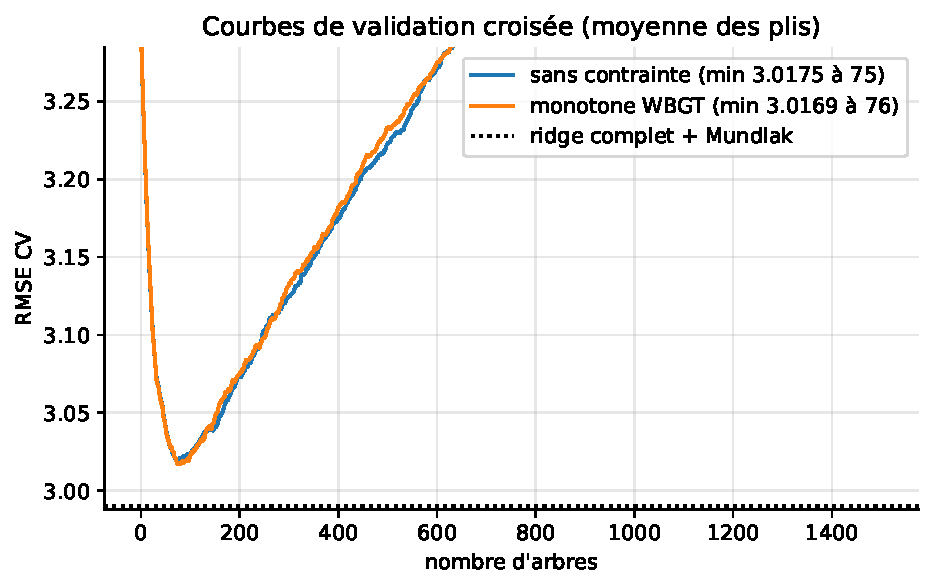
\includegraphics[width=0.62\textwidth]{gbm_cv}
\caption{RMSE de validation croisée par lieux du gradient boosting selon le nombre d'arbres (moyenne des cinq plis),
sans contrainte et avec contrainte de monotonie en WBGT. La ligne pointillée indique la RMSE du ridge complet avec
terme de Mundlak.}
\label{fig:gbm_cv}
\end{figure}

Les deux courbes tombent rapidement pendant les premières dizaines d'arbres, atteignent leur minimum vers 75 arbres,
puis remontent régulièrement (figure~\ref{fig:gbm_cv}) : vers 600 arbres, la RMSE dépasse 3,25 et rejoint la valeur
obtenue avec un seul arbre. Avec un taux d'apprentissage de 0,03, 75 arbres correspondent à peu près au nombre
nécessaire pour capter l'essentiel d'un signal simple : le modèle s'arrête dès qu'il a appris les régularités
générales. Au-delà, chaque arbre apprend des particularités des lieux d'apprentissage, qui ne se transposent pas aux
lieux de validation, et le surapprentissage est rapide.

Deux enseignements en sont ressortis. D'abord, la contrainte de monotonie ne coûte rien : le modèle monotone obtient
une RMSE de 3,0169 avec 76 arbres, contre 3,0175 avec 75 arbres sans contrainte. Imposer que la chaleur ne fasse
jamais courir plus vite ne contredit donc pas les données, et l'on peut injecter cette connaissance physiologique
sans perte de précision. Ensuite, le boosting ne fait pas mieux que les modèles linéaires : avec 3,017, il fait jeu
égal avec le modèle mixte (3,013) et légèrement moins bien que le ridge (2,990 à 2,996), des écarts inférieurs à
0,03 alors que l'erreur type entre plis vaut environ 0,19. La flexibilité des arbres n'apporte rien de mesurable. Le
signal qui se transpose d'un lieu à l'autre est donc essentiellement lisse et proche de l'additif (effets de l'âge,
du niveau, de la forme, de la durée), ce que les modèles linéaires captent déjà ; les non-linéarités et les
interactions que les arbres pourraient découvrir sont soit absentes, soit trop faibles pour être distinguées du bruit
avec quelque 300 courses.

\subsection{Le WBGT résume-t-il bien la météo ? Que coûte une validation mal construite ?}\label{sec:meteo_brute}

Deux expériences ont complété l'étude du boosting, avec un nombre d'arbres choisi à chaque fois par la courbe de
validation croisée. La première compare quatre jeux de variables météorologiques, les autres variables restant les
mêmes : le WBGT accompagné du vent et de la pluie ; les composantes brutes (température de l'air, humidité, vent,
rayonnement, pluie) ; le WBGT et ses composantes ; et aucune variable météorologique. Deux hypothèses s'opposaient.
Si le résumé physique du WBGT perd de l'information utile, par exemple si l'humidité pèse plus que ne le dit la
formule \eqref{eq:wbgt}, les composantes brutes devraient mieux prédire ; si au contraire ce résumé est pertinent, il
devrait faire au moins aussi bien avec moins de variables, donc moins de façons de surapprendre.

Les quatre jeux tiennent en 0,01 de RMSE : 3,017 avec le WBGT, 3,008 avec les composantes brutes comme avec le WBGT et
ses composantes, et 3,014 sans aucune variable météorologique. Le modèle sans météo fait donc aussi bien que le modèle
avec le WBGT, et l'avantage des composantes brutes, vingt fois plus petit que l'erreur type entre plis, ne permet de
conclure ni que le WBGT perd de l'information, ni qu'il la résume bien. Sur ces données, on ne peut pas départager les
jeux de variables par leur pouvoir prédictif.

Ce résultat ne contredit pas l'effet de la chaleur estimé en section~\ref{sec:quel_estimateur}, d'environ 2~points de
$y$ pour 10~°C. Il illustre la différence entre \emph{estimer un effet} et \emph{améliorer une prédiction}. Si la
chaleur agit avec une pente $b \approx 0{,}2$~point par degré et que le WBGT varie avec un écart-type d'environ
4,4~°C, la variance de $y$ due à la chaleur vaut au plus $b^2\,\Var(W) \approx 0{,}04 \times 19{,}5 \approx 0{,}8$.
Rapportée à une variance résiduelle d'environ $3^2 = 9$, elle ferait baisser la RMSE d'au plus
$\sqrt{9} - \sqrt{9 - 0{,}8} \approx 0{,}8/(2 \times 3) \approx 0{,}13$, et seulement si l'effet était connu
parfaitement. Le gain réel est bien plus faible, pour trois raisons : une grande partie de la variation du WBGT est
déjà expliquée par le groupe d'épreuves et l'heure, piste chaude le soir et marathon frais le matin ; l'effet est
hétérogène, fort au marathon et nul en demi-fond, où se trouve la moitié des courses chaudes ; et l'effet est estimé
sur quelque 300 courses, dont peu de chaudes, si bien que l'erreur d'estimation absorbe une partie du gain. Un gain
potentiel de quelques centièmes, noyé dans une variabilité entre plis de 0,19, est invisible en validation croisée.
La qualité de l'outil se jugera donc sur l'estimation de l'effet et sur son incertitude, et non sur la RMSE.

La seconde expérience compare, pour le même modèle, la validation croisée par lieux et une validation croisée
aléatoire à cinq plis sur les lignes. Avec des plis aléatoires, la RMSE annoncée tombe à 2,378, soit une performance
surestimée de 21~\%, et le nombre d'arbres retenu atteint 1\,498, à la limite de la recherche : vingt fois plus qu'avec
les plis par lieux. Avec des plis aléatoires, chaque course a des coureurs en apprentissage et en validation ; le
modèle peut alors mémoriser l'effet propre de chaque course (sa date, son lieu, sa météo, son plateau, son déroulement)
et le restituer aux coureurs de la même course en validation. Plus il ajoute d'arbres, plus il mémorise finement, et
plus il « prédit » bien : la courbe de validation ne remonte plus. Un modèle sélectionné ainsi serait doublement
trompeur : sa performance annoncée serait fausse, et son nombre d'arbres, choisi pour mémoriser, le rendrait fortement
surajusté sur un lieu nouveau, c'est-à-dire exactement dans l'usage prévu de l'outil. La
figure~\ref{fig:gbm_cv} montre ce que coûtent 1\,500 arbres sur des lieux nouveaux : c'est la confirmation empirique
de la fuite d'information décrite en section~\ref{sec:fuites}.

\section{Une troisième famille : les réseaux de neurones}\label{sec:reseaux}

Nous avions jusqu'ici deux grandes familles de modèles : des modèles linéaires, dont la forme est fixée à l'avance,
et des arbres, flexibles mais en marches d'escalier. Les réseaux de neurones forment une troisième famille, flexible
comme les arbres mais produisant des fonctions lisses. Leur forme lisse pourrait convenir à des effets réguliers comme
ceux de l'âge, du niveau ou du WBGT, que les arbres découpent en marches. Nous les présentons sans supposer de
connaissance préalable.

\subsection{Qu'est-ce qu'un réseau de neurones ?}\label{sec:mlp}

Comme tous les modèles de cette étude, un réseau de neurones est une fonction paramétrée $f_\theta$ qui associe une
prédiction $\hat y = f_\theta(x)$ à un vecteur de variables $x$, et dont les paramètres $\theta$ sont appris en
minimisant une perte sur des exemples. Sa particularité est d'appartenir à une famille de fonctions très riche : avec
assez de paramètres, il peut représenter presque n'importe quelle relation entre $x$ et $y$, sans qu'il faille en
préciser la forme. Les réseaux de neurones sont à l'origine des progrès récents en reconnaissance d'images, en
traduction automatique ou en génération de texte, des problèmes où les données sont massives et non structurées et
où personne ne sait écrire à la main la forme de la relation. Ils s'appliquent aussi aux données tabulaires comme les
nôtres, mais avec moins de succès.

L'unité de base est le \emph{neurone}, qui calcule une combinaison linéaire de ses entrées puis lui applique une
fonction non linéaire $\sigma$, appelée \emph{activation} :
\[
h = \sigma\Big(\sum_{r=1}^{d} w_r\,x_r + b\Big) = \sigma(w^\top x + b),
\]
où les $w_r$ sont les \emph{poids} et $b$ le \emph{biais}. Dans cette section, $\sigma$ désigne une fonction
d'activation et non un écart-type. Un neurone n'a rien de mystérieux : si $\sigma$ est l'identité, c'est exactement
une régression linéaire ; si $\sigma$ est la sigmoïde $z \mapsto 1/(1 + e^{-z})$, c'est une régression logistique.

Un réseau assemble des neurones en \emph{couches}. Une couche de $m$ neurones recevant tous le même vecteur
$h \in \mathbb{R}^{d}$ s'écrit $h' = \sigma(W h + b)$, avec $W \in \mathbb{R}^{m \times d}$ et $b \in \mathbb{R}^{m}$,
chaque ligne de $W$ contenant les poids d'un neurone et $\sigma$ s'appliquant composante par composante. Le
\emph{perceptron multicouche} enchaîne $L$ couches, la sortie de l'une étant l'entrée de la suivante :
\begin{equation}\label{eq:mlp}
h_0 = x, \qquad h_k = \sigma(W_k\, h_{k-1} + b_k) \quad (k = 1, \dots, L), \qquad \hat y = w_{L+1}^\top h_L + b_{L+1} .
\end{equation}
Les couches intermédiaires sont dites \emph{cachées}, car on n'observe ni leurs entrées ni leurs sorties. Le nombre de
neurones d'une couche est sa \emph{largeur}, le nombre de couches la \emph{profondeur} du réseau. Une couche qui
reçoit $d$ entrées et compte $m$ neurones a $(d + 1)\,m$ paramètres : leur nombre croît vite avec la largeur.

Sans activation, un réseau ne serait qu'une régression linéaire déguisée, puisque la composition de deux fonctions
affines est affine : $W_2(W_1 x + b_1) + b_2 = (W_2 W_1)\,x + (W_2 b_1 + b_2)$. C'est l'activation qui donne au
réseau sa capacité à représenter des relations non linéaires. La sigmoïde est lisse mais sa dérivée devient très
faible pour $\lvert z \rvert$ grand, ce qui ralentit l'apprentissage des réseaux profonds. L'activation ReLU,
$\max(0, z)$, de dérivée 0 ou 1, fait du réseau une fonction affine par morceaux. L'activation SiLU,
$z \mapsto z\,\mathrm{sig}(z)$ où $\mathrm{sig}$ est la sigmoïde, en est une version lisse et dérivable partout, et
c'est celle que nous utilisons. L'activation ReLU donne une intuition géométrique de la puissance des réseaux. Chaque
neurone de la première couche « plie » l'espace le long de l'hyperplan $w^\top x + b = 0$ : il vaut 0 d'un côté et
croît linéairement de l'autre. En dimension un, une somme $\sum_k c_k \max(0, x - s_k)$ est une ligne brisée dont les
coudes sont placés en $s_k$ et dont la pente change de $c_k$ à chaque coude ; avec assez de coudes, une ligne brisée
approche n'importe quelle courbe continue. C'est l'idée du théorème suivant.

\begin{theoreme}[approximation universelle ; \citealp{cybenko1989, hornik1991, leshno1993}]
Soit $\sigma$ une fonction d'activation continue et non polynomiale. Pour toute fonction continue $g$ définie sur un
compact $K \subset \mathbb{R}^d$ et pour tout $\varepsilon > 0$, il existe un réseau à une seule couche cachée de $N$
neurones,
\[
f_N(x) = \sum_{k=1}^{N} c_k\,\sigma(w_k^\top x + b_k),
\]
tel que $\sup_{x \in K} \lvert g(x) - f_N(x) \rvert < \varepsilon$.
\end{theoreme}

Ce théorème dit qu'aucune relation continue n'est hors de portée d'un réseau assez large. Il faut aussi savoir ce
qu'il ne dit pas. Il garantit l'existence de poids qui conviennent, mais ne dit pas comment les trouver. Le nombre de
neurones nécessaire peut être gigantesque. Il porte sur l'approximation d'une fonction connue sur tout $K$, et non sur
l'apprentissage à partir d'un échantillon fini et bruité : un réseau capable de tout représenter est aussi capable de
représenter le bruit, c'est-à-dire de surapprendre. Enfin, il ne dit rien du comportement hors de $K$ : un réseau
n'extrapole pas de façon fiable. Le théorème n'utilise qu'une couche cachée, mais la profondeur est souvent plus
économe : certaines fonctions exigent un nombre exponentiel de neurones avec une seule couche, et seulement un nombre
polynomial avec plusieurs couches \citep{telgarsky2016}.

\subsection{Comment un réseau apprend}\label{sec:retropropagation}

On cherche les paramètres $\theta$ (toutes les matrices $W_k$ et tous les biais) qui minimisent le risque empirique,
ici l'erreur quadratique moyenne $\hat{\mathcal R}(\theta) = \frac1n\sum_i (y_i - f_\theta(x_i))^2$. Contrairement aux
moindres carrés, il n'existe pas de formule fermée, et la fonction à minimiser n'est pas convexe : elle a de nombreux
minima locaux et points-selles. On procède par descente de gradient, en partant de poids tirés au hasard et en
avançant pas à pas dans la direction opposée au gradient, $\theta \leftarrow \theta - \eta\,\nabla_\theta
\hat{\mathcal R}(\theta)$, où $\eta$ est le taux d'apprentissage. Trop grand, les pas font diverger l'optimisation ;
trop petit, elle est très lente. Rien ne garantit d'atteindre le minimum global, mais en pratique les minima atteints
sont souvent bons. Le résultat dépend toutefois du tirage initial : deux apprentissages avec des graines aléatoires
différentes donnent deux réseaux différents.

Il faut calculer le gradient de la perte par rapport à des milliers de paramètres. La \emph{rétropropagation} le fait
efficacement par la règle de dérivation des fonctions composées, appliquée couche par couche de la sortie vers
l'entrée. Prenons un réseau à une couche cachée, $z = W_1 x + b_1$, $h = \sigma(z)$, $\hat y = w_2^\top h + b_2$, et
la perte d'une observation $\ell = \frac12(\hat y - y)^2$. En notant $\delta = \hat y - y$ l'erreur de prédiction et
$\odot$ le produit composante par composante,
\[
\frac{\partial \ell}{\partial b_2} = \delta, \quad
\frac{\partial \ell}{\partial w_2} = \delta\,h, \quad
\frac{\partial \ell}{\partial z} = (\delta\,w_2) \odot \sigma'(z), \quad
\frac{\partial \ell}{\partial W_1} = \frac{\partial \ell}{\partial z}\,x^\top, \quad
\frac{\partial \ell}{\partial b_1} = \frac{\partial \ell}{\partial z} .
\]
L'erreur $\delta$ est propagée en arrière à travers les poids $w_2$, puis multipliée par la dérivée de l'activation.
Le calcul réutilise les quantités de la passe avant et coûte à peu près autant qu'une prédiction. On comprend aussi
pourquoi la sigmoïde gêne les réseaux profonds : sa dérivée, inférieure à $1/4$, est multipliée une fois par couche, et
le gradient s'éteint en remontant vers l'entrée.

Calculer le gradient sur toutes les données à chaque pas serait coûteux. On le calcule plutôt sur un \emph{mini-lot}
de $n_{\text{lot}}$ observations tirées au hasard (128 ou 256 ici). Le gradient d'un mini-lot est un estimateur sans
biais du gradient complet, plus bruité mais beaucoup moins coûteux, et ce bruit aide même à sortir des minima locaux
médiocres et des points-selles. Une \emph{époque} est un passage complet sur les données, en mini-lots tirés dans un
ordre aléatoire.

Avec un taux d'apprentissage unique, les paramètres dont le gradient est grand avancent trop vite, et ceux dont le
gradient est petit trop lentement. L'optimiseur Adam \citep{kingma2015} adapte le pas de chaque paramètre à partir de
deux moyennes mobiles, celle du gradient $g_t$ et celle de son carré :
\[
m_t = \beta_1 m_{t-1} + (1 - \beta_1)\,g_t, \qquad v_t = \beta_2 v_{t-1} + (1 - \beta_2)\,g_t^2, \qquad
\theta_t = \theta_{t-1} - \eta\,\frac{\hat m_t}{\sqrt{\hat v_t} + \epsilon},
\]
où $\hat m_t = m_t/(1 - \beta_1^t)$ et $\hat v_t = v_t/(1 - \beta_2^t)$ corrigent le biais dû à l'initialisation des
moyennes à 0, avec par défaut $\beta_1 = 0{,}9$ et $\beta_2 = 0{,}999$. Le rapport $\hat m_t/\sqrt{\hat v_t}$ est de
l'ordre de 1 quand le gradient est régulier et plus petit quand il est bruité : chaque paramètre avance d'environ
$\eta$ dans une direction stable, et prudemment dans une direction incertaine.

Un réseau a beaucoup de paramètres : celui que nous utilisons en compte environ 11\,000, pour quelque 6\,400
performances d'apprentissage. Il peut donc, en principe, mémoriser les données d'apprentissage, bruit compris, et doit
être régularisé. Nous avons combiné trois régularisations. Le \emph{weight decay} découplé \citep{loshchilov2019}
rétrécit les poids vers 0 à chaque pas, $\theta \leftarrow \theta - \eta\,\lambda\,\theta$, comme une régression
ridge ; avec Adam, cette version découplée diffère d'une pénalité $\lambda\lVert\theta\rVert^2$ ajoutée à la perte,
dont le gradient serait divisé par $\sqrt{\hat v_t}$ et donc appliqué très inégalement aux paramètres. Le
\emph{dropout} \citep{srivastava2014} met à zéro chaque neurone d'une couche cachée avec une probabilité $p$,
indépendamment à chaque mini-lot, les neurones conservés étant multipliés par $1/(1 - p)$ pour que l'espérance de la
sortie ne change pas. Le réseau ne peut alors compter sur aucun neurone particulier, ni sur une combinaison fragile de
neurones, et l'effet est proche d'une moyenne d'un très grand nombre de sous-réseaux ; en prédiction, tous les
neurones sont utilisés. L'\emph{arrêt précoce}, enfin, mesure la perte de validation à chaque époque, garde les poids
qui l'ont rendue minimale, et arrête l'apprentissage après un nombre fixé d'époques sans amélioration, la
\emph{patience}.

\subsection{Le réseau retenu}\label{sec:architecture}

Un réseau ne traite que des nombres. Pour une variable catégorielle, nous avons utilisé des \emph{embeddings} plutôt
que l'encodage \emph{one-hot}. Un embedding associe à chaque modalité $m$ un vecteur appris $e_m \in \mathbb{R}^{d_e}$,
rangé dans une table $E$ à raison d'une ligne par modalité. C'est équivalent à multiplier l'encodage one-hot de la
modalité par $E$, soit $e_m = E^\top \mathbb 1_m$, c'est-à-dire à une première couche linéaire sans biais appliquée au
one-hot. Les vecteurs sont appris en même temps que le reste du réseau, et deux modalités aux effets proches
finissent avec des vecteurs proches. Pour une variable à très nombreuses modalités, un embedding de petite dimension
résume des milliers de colonnes one-hot en un vecteur dense qui partage l'information entre modalités semblables. Nos
variables catégorielles n'ont que 5 et 2 modalités, si bien que l'embedding n'apporte pas grand-chose ici ; une
modalité inconnue à l'apprentissage reçoit un vecteur réservé.

Notre réseau est un perceptron multicouche dont l'entrée concatène les variables numériques standardisées et un
embedding par variable catégorielle :
\[
h_0 = \big(x^{\text{num}},\ e_{\text{groupe}},\ e_{\text{sexe}}\big),\qquad
h_k = \mathrm{Dropout}\big(\mathrm{SiLU}(W_k\, h_{k-1} + b_k)\big),\qquad \hat y = w_{L+1}^\top h_L + b_{L+1} .
\]
Les variables numériques sont celles du boosting (niveau, âge, forme, durée, altitude, heure, WBGT, vent, pluie et
WBGT moyen du parcours), plus les indicatrices de manquant de l'âge et de la forme, soit 12 colonnes. L'embedding du
groupe d'épreuves est de dimension 4 et celui du sexe de dimension 3, si bien que $h_0$ a 19 composantes. La cible
est elle aussi standardisée sur l'apprentissage, puis les prédictions sont ramenées à l'échelle de $y$. Pour une
architecture à deux couches cachées de 128 et 64 neurones, le réseau compte $(19 + 1) \times 128 = 2\,560$ paramètres
pour la première couche, $(128 + 1) \times 64 = 8\,256$ pour la seconde, $65$ pour la sortie et $33$ pour les deux
tables d'embedding, soit 10\,914 paramètres.

Deux réseaux entraînés avec des graines différentes donnent des prédictions différentes : c'est une source de variance
propre à l'optimisation non convexe. Nous moyennons donc les prédictions de $n_{\text{mod}}$ réseaux entraînés avec
des graines différentes. Si ces prédicteurs ont chacun une variance $s^2$ et une corrélation $\rho$ deux à deux, leur
moyenne a pour variance
\[
\Var\Big(\frac{1}{n_{\text{mod}}}\sum_{m=1}^{n_{\text{mod}}} f_m\Big) = \rho\,s^2 + \frac{1 - \rho}{n_{\text{mod}}}\,s^2 ,
\]
qui baisse avec $n_{\text{mod}}$ tant que les réseaux ne sont pas parfaitement corrélés, sans aucun coût en biais.

\subsection{Le surapprentissage, observé}\label{sec:surapprentissage}

Pour voir le surapprentissage à l'œuvre, nous avons d'abord entraîné un réseau de 128 et 64 neurones, sans dropout ni
weight decay, avec un taux d'apprentissage de $3\cdot10^{-3}$, sur quatre plis de lieux, en suivant l'erreur sur le
cinquième pli, formé de quatorze lieux nouveaux.

\begin{figure}[htbp]
\centering
\begin{minipage}[t]{0.49\textwidth}
\centering
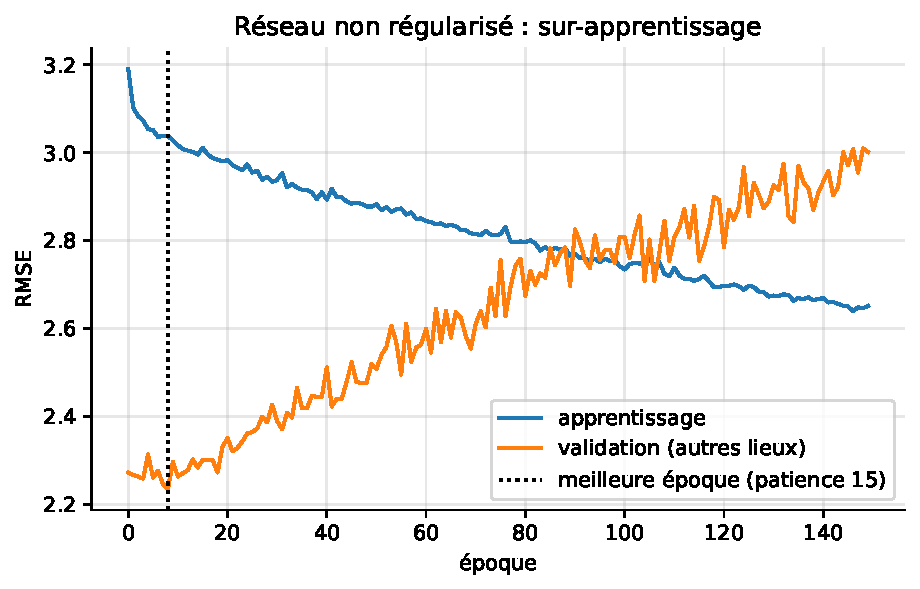
\includegraphics[width=\linewidth]{reseau_surapprentissage}
\end{minipage}\hfill
\begin{minipage}[t]{0.49\textwidth}
\centering
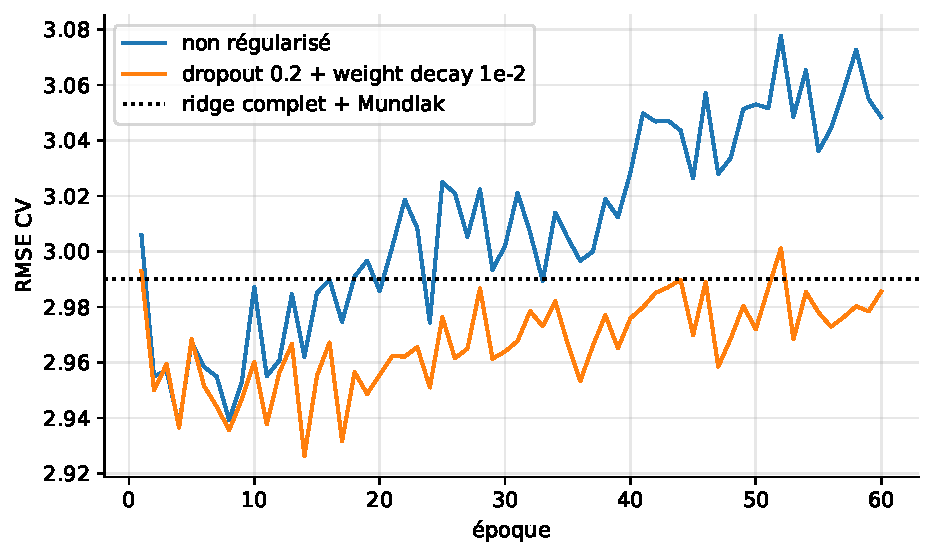
\includegraphics[width=\linewidth]{reseau_cv}
\end{minipage}
\caption{À gauche, RMSE d'apprentissage (quatre plis) et de validation (pli~0, lieux nouveaux) d'un réseau non
régularisé au fil des époques ; la ligne pointillée marque la meilleure époque de validation. À droite, RMSE de
validation croisée (moyenne des trois premiers plis) selon le nombre d'époques, sans régularisation et avec dropout
et weight decay ; la ligne pointillée indique la RMSE du ridge complet sur les cinq plis.}
\label{fig:reseau}
\end{figure}

La figure~\ref{fig:reseau} (à gauche) montre la signature typique du surapprentissage. La RMSE d'apprentissage baisse
sans interruption, de 3,19 à la première époque à 2,65 à la 150\textsuperscript{e} : le réseau s'ajuste de mieux en
mieux aux lieux qu'il voit. La RMSE de validation atteint au contraire son minimum dès la 9\textsuperscript{e} époque,
puis remonte presque linéairement jusqu'à 3,00. À partir de là, chaque époque améliore l'ajustement aux lieux
d'apprentissage au détriment des lieux nouveaux : avec environ 11\,000 paramètres pour 6\,435 performances
d'apprentissage, le réseau a largement de quoi mémoriser le bruit et les particularités de chaque lieu. L'arrêt précoce,
avec une patience de 15 époques, interrompt l'apprentissage à la 24\textsuperscript{e} époque et recharge les poids de
la 9\textsuperscript{e} : la RMSE de validation vaut alors 2,235, contre 3,002 à la fin de l'apprentissage. Le
surapprentissage coûte donc 0,77~point de RMSE, soit $34$~\% ; sans arrêt précoce, le réseau fait même nettement moins
bien que le modèle constant sur ce pli (2,647). Que l'erreur de validation soit d'abord inférieure à l'erreur
d'apprentissage n'a rien d'un paradoxe : le pli~0 est le plus facile des cinq, ses lieux ayant des performances moins
dispersées, et c'est l'évolution des deux courbes qui compte. La valeur 2,235 est d'ailleurs optimiste, l'époque
d'arrêt ayant été choisie sur ce même pli, au point le plus bas d'une courbe bruitée.

Comme pour le boosting, nous avons donc choisi le nombre d'époques sur la courbe de validation croisée moyenne. Faute
de temps de calcul, cette recherche porte sur les trois premiers plis et 60 époques au plus, pour deux réglages d'un
réseau de 128 et 64 neurones avec un taux d'apprentissage de $10^{-3}$ : sans régularisation, et avec dropout
($p = 0{,}2$) et weight decay ($\lambda = 10^{-2}$). Le réseau non régularisé atteint son minimum dès la
4\textsuperscript{e} époque (RMSE de 2,937), puis remonte au-delà de 3,05 à partir de la 40\textsuperscript{e} ; le
réseau régularisé atteint le sien à la 14\textsuperscript{e} époque (2,926), et sa courbe reste entre 2,93 et 3,00
pendant les 60 époques (figure~\ref{fig:reseau}, à droite). La régularisation n'améliore presque pas la meilleure
valeur, mais elle rend le réseau beaucoup moins sensible au nombre d'époques, ce qui est précieux puisque ce nombre
est choisi sur une courbe bruitée.

La comparaison avec les autres modèles demande une précaution : les trois premiers plis sont plus faciles que la
moyenne, et il faut confronter le réseau aux autres modèles sur les mêmes plis. Le ridge complet y obtient 2,936 sans
terme de Mundlak et 2,938 avec, le modèle mixte 2,977 et le modèle constant 3,281. La ligne pointillée de la figure,
qui représente le ridge sur les cinq plis, flatte donc le réseau : à plis égaux, le réseau régularisé ne devance le
ridge que de 0,01, et le réseau non régularisé fait jeu égal avec lui. Ces écarts sont très inférieurs à l'erreur type
entre plis, d'autant que les courbes oscillent de 0,02 à 0,03 d'une époque à l'autre : le réseau ne fait pas mieux
qu'un modèle linéaire bien spécifié. C'est le résultat attendu sur des données tabulaires de taille modeste
\citep{grinsztajn2022}, et il confirme le diagnostic tiré du boosting : le signal qui se transpose d'un lieu à
l'autre est lisse et presque additif, et un modèle linéaire le capte déjà.

On aurait pu, enfin, apprendre un embedding par course ou par lieu, l'équivalent neuronal d'un intercept aléatoire.
Ce serait inutile ici : toutes les courses et tous les lieux évalués sont nouveaux, et leur vecteur n'aurait jamais
été appris. C'est le problème du \emph{démarrage à froid}, le même qui annule le BLUP du modèle mixte en validation.
Le record personnel joue déjà le rôle de l'effet individuel de l'athlète, mesuré hors de la course.

\section{Régler, puis comparer sur des villes jamais vues}\label{sec:comparaison}

Nous disposions à ce stade de quatre familles de modèles, construites avec des réglages de départ raisonnables. Deux
questions restaient ouvertes : peut-on améliorer ces modèles en réglant mieux leurs hyperparamètres ? Et, une fois
chaque modèle réglé, lequel est le meilleur, avec quelle certitude ? Pour répondre à la seconde, nous avons utilisé
pour la première et unique fois l'ensemble de test mis de côté au début de l'étude.

\subsection{La recherche aléatoire des hyperparamètres}\label{sec:recherche}

Un modèle a deux sortes de réglages. Les \emph{paramètres} sont appris à partir des données par l'algorithme lui-même :
coefficients d'une régression, valeurs des feuilles d'un arbre, poids d'un réseau. Les \emph{hyperparamètres} sont
fixés avant l'apprentissage et en déterminent la forme ou l'intensité : taux d'apprentissage, nombre de feuilles,
pénalité, architecture d'un réseau, taux de dropout. Ils règlent surtout la complexité du modèle, c'est-à-dire le
compromis entre biais et variance, et ne peuvent pas être appris en minimisant l'erreur d'apprentissage, qui
choisirait toujours le modèle le plus complexe. On les choisit donc en minimisant une estimation de l'erreur sur des
données non vues, ici la RMSE de validation croisée par lieux.

La recherche sur grille essaie toutes les combinaisons d'un ensemble de valeurs fixé pour chaque hyperparamètre. Avec
$q$ hyperparamètres et $k$ valeurs chacun, il faut $k^q$ évaluations : 5 valeurs pour 7 hyperparamètres demandent déjà
$5^7 = 78\,125$ validations croisées. La recherche aléatoire tire au hasard $N$ configurations dans l'espace de
recherche. \citet{bergstra2012} ont montré qu'à budget égal elle explore mieux qu'une grille, pour une raison simple :
en pratique, seuls quelques hyperparamètres comptent vraiment, et l'on ne sait pas d'avance lesquels. Une grille de
$N$ points n'essaie que $N^{1/q}$ valeurs distinctes de chaque hyperparamètre, alors qu'un tirage aléatoire en essaie
$N$ de chacun. Elle offre de plus une garantie simple. Appelons « bonne » une configuration située dans les 5~\%
meilleures de l'espace de recherche. Chaque tirage a une probabilité $0{,}05$ d'en être une, donc la probabilité
qu'au moins un des $N$ tirages soit bon vaut $1 - 0{,}95^N$, qui dépasse 95~\% dès $N = 60$, quelle que soit la
dimension de l'espace. Avec nos budgets, 16 tirages donnent une probabilité de 56~\% d'atteindre les 5~\% meilleures
configurations, et de 81~\% d'atteindre les 10~\% meilleures.

Chaque hyperparamètre est tiré selon une loi adaptée à sa nature. Pour les paramètres d'échelle, comme les taux
d'apprentissage et les pénalités, dont l'effet dépend de l'ordre de grandeur plutôt que de la valeur absolue, nous
utilisons une loi \emph{log-uniforme} : on tire $U$ uniformément sur $[\ln a\,;\,\ln b]$ et l'on prend $x = e^U$. La
densité de $x$ est alors $1/\big(x \ln(b/a)\big)$ sur $[a\,;\,b]$, et
\[
\mathbb{P}(x \leq c) = \frac{\ln(c/a)}{\ln(b/a)},
\]
si bien que chaque ordre de grandeur reçoit la même probabilité : sur $[0{,}001\,;\,0{,}1]$,
$\mathbb{P}(x < 0{,}01) = 1/2$. Avec une loi uniforme sur $[0{,}01\,;\,0{,}1]$ au contraire, 56~\% des tirages
tomberaient au-dessus de 0,05 et 11~\% seulement sous 0,02 : les petites valeurs, souvent les meilleures, ne seraient
presque jamais essayées. Les proportions suivent une loi uniforme, les effectifs une loi uniforme sur les entiers, et
les options discrètes un choix uniforme dans une liste.

Pour le gradient boosting, 16 configurations ont été tirées, chacune évaluée sur les cinq plis avec la contrainte de
monotonie et un nombre d'arbres choisi par la courbe moyenne : taux d'apprentissage log-uniforme entre 0,02 et 0,1,
nombre de feuilles entre 4 et 48, effectif minimal par feuille entre 20 et 250, pénalité $\lambda$ log-uniforme entre
0,1 et 50, fractions de variables et de lignes uniformes entre 0,5 et 1, et gain minimal $\kappa$ parmi 0, $0{,}001$ et
$0{,}01$. Pour le réseau, plus coûteux, 5 configurations ont été évaluées sur trois plis : architecture parmi une
couche de 32 neurones, deux couches de 64 et 32 ou de 128 et 64, et trois couches de 64, 64 et 32 ; dropout uniforme
entre 0 et 0,3 ; taux d'apprentissage log-uniforme entre $3\cdot10^{-4}$ et $3\cdot10^{-3}$ ; weight decay
log-uniforme entre $10^{-5}$ et $3\cdot10^{-2}$ ; dimension des embeddings parmi 2, 4 et 8 ; mini-lots de 128 ou 256.

Choisir la meilleure de $N$ configurations sur la RMSE de validation croisée introduit un \emph{biais de sélection}.
Chaque RMSE estimée contient une part de bruit, et la configuration retenue est celle dont l'estimation est la plus
basse, ce qui favorise celles dont le bruit a été favorable :
\[
\E\Big[\min_{k \leq N} \widehat{\mathrm{RMSE}}_k\Big] \leq \min_{k \leq N} \E\big[\widehat{\mathrm{RMSE}}_k\big] .
\]
C'est la même inégalité que pour le choix du nombre d'arbres, à l'échelle de la configuration entière. Dans le cas le
plus simple, où $N$ configurations auraient la même erreur réelle et des erreurs d'estimation indépendantes de même
écart-type $s$, la plus favorable serait en moyenne inférieure de $1{,}8\,s$ à l'erreur réelle pour $N = 16$ :
c'est l'espérance du maximum de 16 variables normales centrées réduites, qui croît comme $\sqrt{2\ln N}$. En
pratique l'effet est plus faible, car toutes les configurations sont évaluées sur les mêmes plis et leurs erreurs
d'estimation sont fortement corrélées. Le score de validation croisée du gagnant reste néanmoins optimiste, et c'est
le rôle de l'ensemble de test que de le corriger.

Pour le gradient boosting, la surface explorée s'est révélée être un plateau. Les six meilleures configurations
tiennent en 0,005 de RMSE alors que leurs hyperparamètres sont très différents, avec des taux d'apprentissage de 0,02
à 0,06 et de 31 à 159 arbres : la valeur précise des hyperparamètres compte très peu, ce qui est exactement la
situation décrite par \citet{bergstra2012}. La meilleure configuration tirée (taux de 0,020, 21 feuilles, au moins 218
performances par feuille, $\lambda = 0{,}12$, 86~\% des variables et 59~\% des lignes par arbre, 159 arbres) obtient
3,0278, un peu moins bien que le réglage de départ (3,0169). Ce réglage appartient pourtant à l'espace de recherche,
mais aucun des seize tirages n'est tombé dans une région aussi bonne, ce qui n'a rien de surprenant avec une chance
sur deux d'atteindre les 5~\% meilleures configurations ; l'écart, de 0,011, est de toute façon sans conséquence
pratique, et nous avons conservé la configuration tirée. Une tendance nette se dégage : cinq des six meilleures
configurations exigent au moins 129 performances par feuille. Une feuille aussi peuplée ne peut isoler ni une course
ni même un petit lieu : ces arbres sont fortement régularisés, ce qui confirme que le signal transposable est lisse.
Le même réglage sans contrainte de monotonie obtient enfin 3,0335 avec 130 arbres : la contrainte ne coûte toujours
rien.

Pour le réseau, les cinq configurations tiennent en 0,018, avec des architectures aussi différentes qu'une seule
couche de 32 neurones et trois couches de 64, 64 et 32. La configuration la moins régularisée (dropout de 0,08, sans
weight decay) est la dernière, et la meilleure, de RMSE 2,922 sur trois plis, a le dropout le plus fort : trois
couches de 64, 64 et 32 neurones, dropout de 0,27, taux d'apprentissage de $1{,}2\cdot10^{-3}$, weight decay de
$3{,}4\cdot10^{-3}$, embeddings de dimension 4, mini-lots de 256 et 14 époques. Le taux d'apprentissage et le nombre
d'époques vont de pair : avec un taux de $3$ à $4\cdot10^{-4}$, il faut 24 à 58 époques pour atteindre le minimum.
Sur les mêmes plis, le ridge obtenait 2,936 à 2,938 : l'avance du meilleur réseau, de 0,015, est très inférieure à
l'erreur type, et en partie l'effet du biais de sélection. Le réseau final moyenne cinq réseaux de ce réglage.

\subsection{L'évaluation finale}\label{sec:test}

Tous les modèles ont été réentraînés sur l'ensemble des 79 lieux d'apprentissage, avec les hyperparamètres choisis
par validation croisée, puis évalués une seule fois sur les 21 lieux de test (2\,355 performances, 102 courses).
Cette évaluation est honnête parce qu'aucun choix n'a été fait en regardant le test. Neuf modèles sont comparés : le
modèle constant ; les moyennes par épreuve et sexe ; les moindres carrés sur le WBGT seul ; le meilleur ridge complet,
avec terme de Mundlak ; le modèle à intercept aléatoire de course retenu par la règle d'un écart-type ; le gradient
boosting réglé, avec et sans contrainte de monotonie ; l'ensemble de cinq réseaux ; et un \emph{ensemble} qui moyenne
les prédictions du modèle mixte, du boosting monotone et des réseaux.

L'idée de ce dernier ensemble repose sur une inégalité de convexité. Si $e_1, e_2, e_3$ sont les erreurs de trois
modèles sur une performance, l'erreur de leur moyenne est la moyenne des erreurs, et
$\big(\frac{e_1 + e_2 + e_3}{3}\big)^2 \leq \frac{e_1^2 + e_2^2 + e_3^2}{3}$ ; en moyennant sur les performances,
\[
\mathrm{MSE}(\text{ensemble}) \leq \frac{\mathrm{MSE}_1 + \mathrm{MSE}_2 + \mathrm{MSE}_3}{3} .
\]
L'ensemble fait toujours au moins aussi bien que la moyenne de ses membres, et d'autant mieux que leurs erreurs sont
peu corrélées. Des modèles de familles différentes se trompent a priori de façons différentes.

Avec 21 lieux seulement, la RMSE de test est elle-même incertaine : un autre tirage de lieux de test donnerait une
autre valeur. Pour quantifier cette incertitude, nous utilisons le \emph{bootstrap} \citep{efron1979}. On voudrait
connaître la distribution d'une statistique sur des échantillons tirés de la population, mais on ne dispose que d'un
échantillon. L'idée du bootstrap est de remplacer la population par l'échantillon lui-même : on tire avec remise,
dans l'échantillon, de nouveaux échantillons de même taille, et l'on recalcule la statistique sur chacun. La
dispersion des $B$ valeurs obtenues imite celle qu'on observerait sur de vrais nouveaux échantillons, et
l'intervalle de confiance percentile à 95~\% est formé des quantiles d'ordre 0,025 et 0,975 des $B$ répliques. Nous
prenons $B = 2\,000$ : un quantile d'ordre 0,025 est alors estimé à partir des 50 répliques les plus extrêmes, ce qui
le rend stable.

Le bootstrap suppose cependant que les unités rééchantillonnées sont indépendantes. Les erreurs de prédiction d'une
même course, et même d'un même lieu, étant corrélées, rééchantillonner les performances une à une sous-estimerait
l'incertitude, exactement comme les erreurs types naïves. Nous rééchantillonnons donc les \emph{lieux} : on tire 21
lieux avec remise parmi les 21 lieux de test, on réunit toutes leurs performances, et l'on recalcule la RMSE. L'unité
de rééchantillonnage est ainsi la même que l'unité de regroupement de la validation. Pour comparer deux modèles $A$
et $B$, enfin, on ne compare pas leurs deux intervalles : on calcule la différence de leurs RMSE sur chacune des
mêmes répliques, puis l'intervalle de cette différence. C'est beaucoup plus précis, car
\[
\Var(R_A - R_B) = \Var(R_A) + \Var(R_B) - 2\,\Cov(R_A, R_B),
\]
et la covariance est fortement positive : un lieu difficile à prédire augmente l'erreur de tous les modèles à la fois.
Si l'intervalle de la différence exclut 0, l'écart est significatif au seuil de 5~\%. Le modèle constant sert de
référence (tableau~\ref{tab:test}).

\begin{table}[htbp]
\centering
\small
\caption{Évaluation finale sur les 21 lieux de test (2\,355 performances). Intervalles de confiance à 95~\% par
bootstrap des lieux ($B = 2\,000$) ; l'écart au modèle constant est calculé réplique par réplique.}
\label{tab:test}
\begin{tabular}{@{}lcccccc@{}}
\toprule
Modèle & RMSE & IC 95~\% & Écart au constant & IC 95~\% de l'écart & $R^2$ & MAE \\
\midrule
ensemble (mixte, boosting, réseaux) & 2,877 & [2,50 ; 3,27] & $-0{,}314$ & [$-0{,}52$ ; $-0{,}17$] & 0,172 & 2,136 \\
mixte (intercept de course) & 2,896 & [2,52 ; 3,29] & $-0{,}295$ & [$-0{,}51$ ; $-0{,}14$] & 0,162 & 2,149 \\
boosting monotone & 2,898 & [2,52 ; 3,29] & $-0{,}294$ & [$-0{,}49$ ; $-0{,}16$] & 0,161 & 2,151 \\
réseaux (ensemble de 5) & 2,902 & [2,51 ; 3,30] & $-0{,}289$ & [$-0{,}50$ ; $-0{,}14$] & 0,158 & 2,160 \\
boosting libre & 2,902 & [2,52 ; 3,30] & $-0{,}289$ & [$-0{,}47$ ; $-0{,}16$] & 0,158 & 2,155 \\
ridge complet avec Mundlak & 2,944 & [2,49 ; 3,41] & $-0{,}247$ & [$-0{,}53$ ; $-0{,}11$] & 0,133 & 2,214 \\
moindres carrés sur le WBGT & 3,142 & [2,73 ; 3,61] & $-0{,}050$ & [$-0{,}14$ ; $+0{,}05$] & 0,013 & 2,383 \\
constant & 3,191 & [2,70 ; 3,71] & 0 & -- & $-0{,}018$ & 2,422 \\
moyennes par épreuve et sexe & 3,305 & [2,78 ; 3,86] & $+0{,}113$ & [$-0{,}03$ ; $+0{,}22$] & $-0{,}092$ & 2,501 \\
\bottomrule
\end{tabular}
\end{table}

Les modèles qui utilisent le profil des athlètes battent nettement le modèle constant : ils réduisent la RMSE de 0,25 à
0,31~point, et tous les intervalles de ces écarts excluent 0. Leur $R^2$ de test va de 0,13 à 0,17 : environ un
sixième de la variance des performances est prévisible sur un lieu jamais vu. Le reste, forme du jour, tactique,
ancienneté du record, ne l'est pas. Les modèles naïfs, eux, ne font pas mieux que la constante. Le WBGT seul gagne
0,05~point, avec un intervalle qui contient 0 : la chaleur, prise seule, ne prédit pas la performance. Les moyennes par
épreuve et sexe font même moins bien que la constante, comme en validation croisée.

L'ordre entre les meilleurs modèles n'est pas établi. Cinq modèles tiennent en 0,025 de RMSE, et le modèle mixte, les
deux boostings et les réseaux en 0,006 ; leurs écarts au modèle constant ont des intervalles qui se chevauchent
presque entièrement. Les familles de modèles sont équivalentes en prédiction. Un renversement mérite toutefois
d'être noté : le ridge, légèrement meilleur en validation croisée, est le moins bon des modèles avec contrôles sur le
test, alors que le modèle mixte, légèrement moins bon en validation croisée, est parmi les meilleurs. Le ridge retenu
est un polynôme de degré~3 avec interactions, choisi par la plus petite RMSE, alors que le modèle mixte est de degré~1,
choisi par la règle d'un écart-type. Ce renversement va dans le sens de notre crainte : un modèle plus complexe,
choisi sur des écarts non significatifs, se transpose moins bien à de nouveaux lieux. L'écart entre les deux, de
0,048, reste cependant trop faible pour le prouver.

L'ensemble est le meilleur modèle, mais gagne peu. Conformément à l'inégalité de convexité, son erreur quadratique
est inférieure à la moyenne de celles de ses trois membres :
\[
2{,}877^2 = 8{,}28 \;<\; \tfrac13\big(2{,}896^2 + 2{,}898^2 + 2{,}902^2\big) = 8{,}40 .
\]
Le gain n'est pourtant que de 1,5~\%, parce que les trois
modèles se trompent presque toujours dans le même sens sur les mêmes performances : la corrélation entre leurs erreurs
est de 0,97 à 0,99. Ce qu'ils ne savent pas prédire, la forme du jour, aucun d'eux ne le sait. De même, les cinq
réseaux de l'ensemble ont, pris séparément, des RMSE de test de 2,89 à 2,92 : moyenner les graines ne rend pas le
réseau meilleur que son meilleur membre, mais évite de dépendre d'une graine malchanceuse.

Les intervalles sont larges : celui de la RMSE de l'ensemble va de 2,50 à 3,27. Il n'y a que 21 lieux, et quelques-uns
pèsent très lourd : Portland compte à lui seul 686 performances (29~\% du test) et Valencia 415 (18~\%). Selon que ces
lieux sont tirés zéro, une ou deux fois dans une réplique, la RMSE change beaucoup. L'intervalle de l'écart au modèle
constant est deux fois plus étroit, parce que la différence élimine la part commune de difficulté. On remarque enfin
que les RMSE de test sont inférieures à celles de validation croisée (2,88 à 2,94 contre 2,99 à 3,03 pour les modèles
avec contrôles, 3,19 contre 3,30 pour la constante) : les lieux de test sont un peu moins hétérogènes que la moyenne
des plis, et ce sont les écarts entre modèles qu'il faut comparer, non les niveaux absolus.

Ce bilan a orienté toute la suite du travail. En prédiction, les quatre familles de modèles se valent : un modèle
linéaire mixte de degré~1 fait aussi bien qu'un boosting réglé ou qu'un ensemble de réseaux. Le choix du modèle de
l'outil ne pouvait donc pas se faire sur la précision des prédictions. Il devait se faire sur la qualité de
l'estimation de l'effet de la chaleur : lisibilité de la courbe de dégradation, absence de biais et incertitude
honnête.

\section{Ce que les modèles ont appris de la chaleur}\label{sec:interpretation}

L'outil n'a pas besoin de la meilleure prédiction d'un chrono, mais d'une estimation fiable de l'\emph{effet} des
conditions météorologiques. Puisque les modèles se valent en prédiction, nous les avons ouverts pour voir ce qu'ils
ont appris. Cette étape a fait apparaître le résultat le plus important de l'étude : des modèles de précision
identique racontent des histoires différentes sur la chaleur.

\subsection{Attribuer une prédiction aux variables : les valeurs de Shapley}\label{sec:shap}

Pour un modèle linéaire, la contribution d'une variable à une prédiction se lit directement : c'est le produit de son
coefficient par sa valeur. Pour un boosting de 159 arbres, il n'existe rien de tel, puisqu'une même variable intervient
dans des centaines de coupures, en interaction avec les autres. La théorie des jeux coopératifs répond pourtant à une
question analogue : comment répartir équitablement le gain d'une coalition entre ses joueurs, quand l'apport de chacun
dépend des autres \citep{shapley1953} ? Les « joueurs » sont ici les $p$ variables, et le « gain » est la prédiction.
Pour une performance $x$, notons $v(S) = \E\big[f(X) \mid X_S = x_S\big]$ la prédiction attendue quand on ne connaît
que les variables de l'ensemble $S$, les autres étant remplacées par leur distribution dans les données ;
$v(\varnothing) = \E[f(X)]$ est la prédiction moyenne et $v(\{1, \dots, p\}) = f(x)$ la prédiction complète. La
\emph{valeur de Shapley} de la variable $j$ est
\begin{equation}\label{eq:shapley}
\phi_j(x) = \sum_{S \subseteq \{1, \dots, p\} \setminus \{j\}} \frac{|S|!\,(p - |S| - 1)!}{p!}\,
\big[v(S \cup \{j\}) - v(S)\big].
\end{equation}
La différence $v(S \cup \{j\}) - v(S)$ est l'apport marginal de $j$ quand il rejoint l'ensemble $S$. Le coefficient
$|S|!\,(p - |S| - 1)!/p!$ est la probabilité que, dans un ordre d'arrivée des variables tiré au hasard parmi les $p!$
ordres possibles, les variables arrivées avant $j$ soient exactement celles de $S$. La valeur de Shapley est donc
l'apport marginal de $j$ moyenné sur tous les ordres d'arrivée : aucun ordre n'est privilégié. Avec deux variables,
par exemple, $\phi_1(x) = \frac12\big[v(\{1\}) - v(\varnothing)\big] + \frac12\big[v(\{1, 2\}) - v(\{2\})\big]$ est la
moyenne de l'apport de la variable~1 quand elle arrive en premier et quand elle arrive en second. Les valeurs de
Shapley sont l'unique répartition qui vérifie quatre propriétés : l'efficacité,
$f(x) = \phi_0 + \sum_{j} \phi_j(x)$ avec $\phi_0 = \E[f(X)]$, qui décompose exactement la prédiction ; la symétrie,
qui donne la même contribution à deux variables jouant le même rôle ; la nullité de la contribution d'une variable
qui ne change jamais la prédiction ; et l'additivité, qui fait s'additionner les contributions d'une somme de modèles,
comme un boosting. La formule demande $2^{p-1}$ termes par variable, mais pour les arbres, l'algorithme TreeSHAP
calcule les valeurs exactes en temps polynomial \citep{lundberg2017, lundberg2020}. Nous l'avons appliqué au boosting
monotone, sur les lieux de test.

\begin{figure}[htbp]
\centering
\begin{minipage}[c]{0.53\textwidth}
\centering
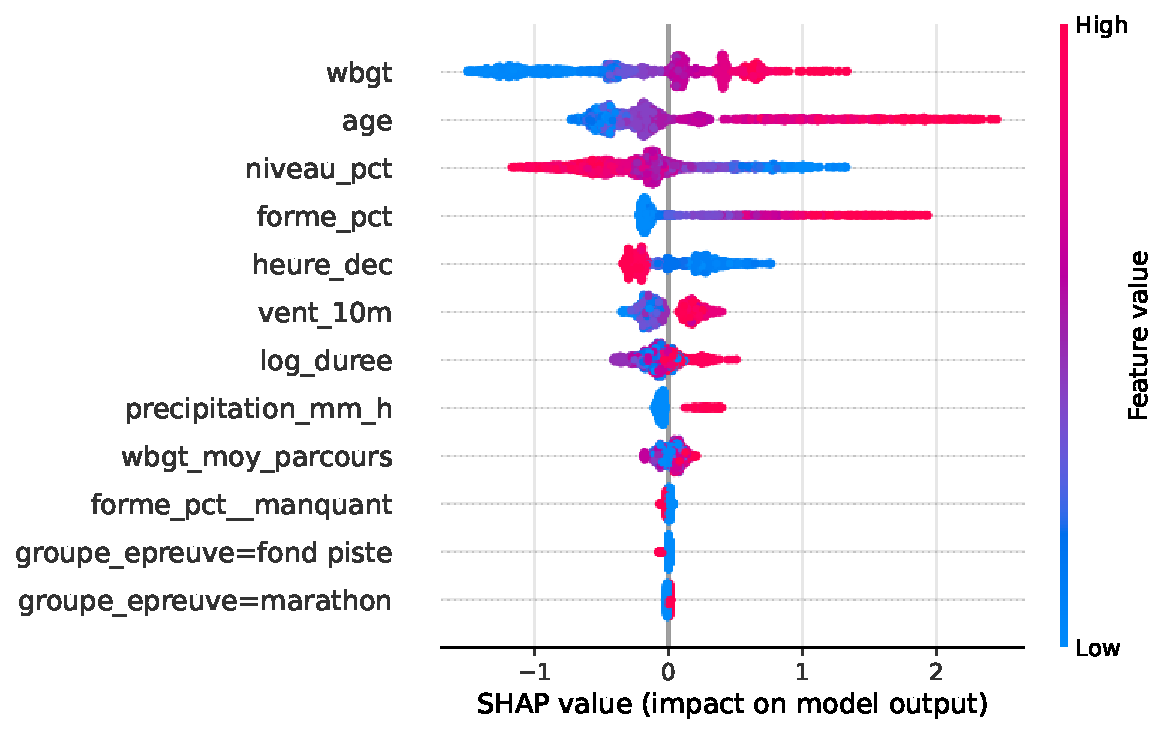
\includegraphics[width=\linewidth]{shap_resume}
\end{minipage}\hfill
\begin{minipage}[c]{0.45\textwidth}
\centering
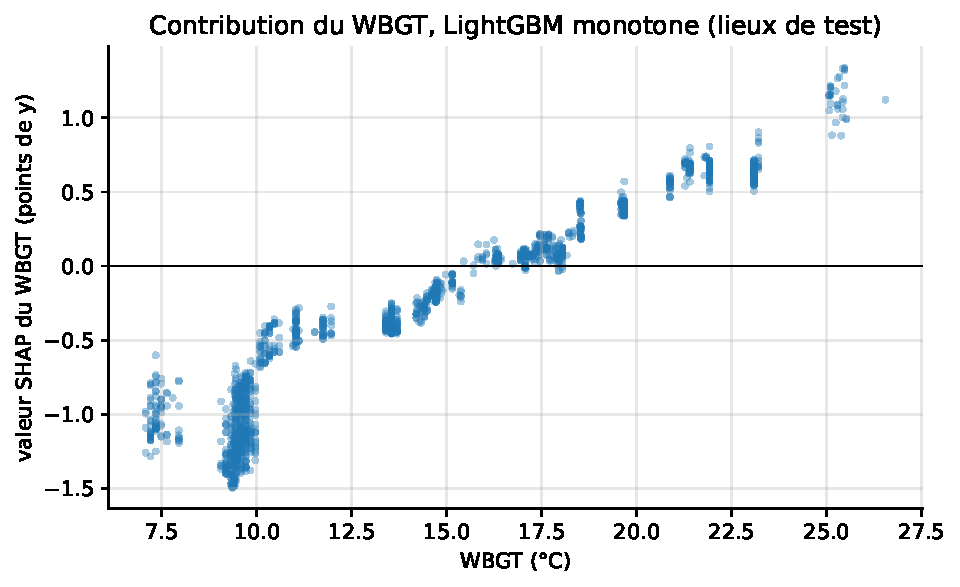
\includegraphics[width=\linewidth]{shap_wbgt}
\end{minipage}
\caption{Valeurs de Shapley du boosting monotone sur les lieux de test. À gauche, une ligne par variable et un point
par performance, coloré selon la valeur de la variable (\texttt{niveau\_pct} : niveau ; \texttt{heure\_dec} : heure de
départ ; \texttt{log\_duree} : logarithme de la durée attendue ; \texttt{wbgt\_moy\_parcours} : WBGT moyen du parcours).
À droite, contribution du WBGT selon sa valeur.}
\label{fig:shap}
\end{figure}

L'importance globale d'une variable est la moyenne de $|\phi_j|$ sur les performances, en points de $y$. Le WBGT est
la variable la plus importante du modèle, avec une contribution moyenne de 0,55~point, devant l'âge (0,50), le niveau
(0,39), la forme (0,29), l'heure (0,24), le vent (0,16), la durée attendue (0,13), la pluie (0,07) et le WBGT moyen du
parcours (0,07) ; les indicatrices de groupe d'épreuves reçoivent des contributions quasi nulles
(figure~\ref{fig:shap}). La contribution du WBGT croît, en marches, de $-1{,}4$~point vers 9,5~°C à $+1{,}2$~point vers
25~°C. Les points y forment des bandes verticales, chaque bande correspondant à une course dont tous les coureurs
partagent le même WBGT ; et les contributions sont mesurées par rapport à la prédiction moyenne $\phi_0$, et non par
rapport au WBGT de référence. Le sens des effets est celui attendu : un WBGT élevé, un âge élevé, une forme éloignée du
record, un vent fort, la pluie et une longue durée ralentissent par rapport au record. Une heure tardive est associée à
des performances plus proches du record, car les réunions de piste du soir offrent pistes rapides et lièvres. Un
athlète plus lent que la médiane de son épreuve court aussi plus près de son record ; plusieurs explications sont
possibles, comme un record moins exceptionnel ou la sélection par la marge de troncature, et le modèle ne permet pas
de les départager.

Ce résultat semble contredire celui de la section~\ref{sec:meteo_brute}, où retirer toutes les variables
météorologiques ne dégradait pas la RMSE. Les deux sont compatibles. Le WBGT est très lié au groupe d'épreuves et à
l'heure : quand il est présent, une partie de l'information qu'il porte pourrait aussi l'être par ces variables, et la
valeur de Shapley lui en attribue le crédit ; quand il est absent, l'heure, la durée et le groupe prennent le relais.
Une forte valeur de Shapley ne signifie ni qu'une variable est indispensable à la prédiction, ni qu'elle a un effet
causal : elle décrit le modèle, pas le monde. Pour mesurer l'effet de la chaleur à profil d'athlète donné, il fallait
un autre outil.

\subsection{Dépendance partielle et courbe de dégradation}\label{sec:pd}

La \emph{dépendance partielle} d'un modèle $f$ en une variable $v$ \citep{friedman2001} est la fonction
\[
\mathrm{PD}_v(\xi) = \frac1n\sum_{i=1}^n f\big(x_i \text{ avec } x_{i,v} = \xi\big) :
\]
pour chaque valeur $\xi$, on impose $x_{i,v} = \xi$ à toutes les performances, les autres variables gardant leurs
valeurs observées, et l'on moyenne les prédictions. C'est la réponse à la question : « que prédirait le modèle, en
moyenne sur nos athlètes et nos courses, si la variable $v$ valait $\xi$ pour tout le monde ? » Contrairement à la
moyenne de $y$ par classe de WBGT, qui compare des courses différentes, la dépendance partielle compare les mêmes
performances sous deux valeurs de la variable : la composition des épreuves, l'âge et le niveau sont identiques d'une
valeur à l'autre, ce qui neutralise le paradoxe de Simpson au sein du modèle. Avant la moyenne, chaque performance
$i$ a sa propre courbe $\xi \mapsto f(x_i \text{ avec } x_{i,v} = \xi)$, dite courbe ICE \citep{goldstein2015}. Leur
dispersion renseigne sur les interactions : si toutes les courbes ICE sont parallèles, l'effet de $v$ est le même pour
toutes les performances ; si elles divergent, il dépend des autres variables.

La courbe de dégradation est la dépendance partielle en WBGT, recentrée sur la référence :
\begin{equation}\label{eq:courbe_degradation}
\Delta(W) = \mathrm{PD}_{\WBGT}(W) - \mathrm{PD}_{\WBGT}(W_{\text{ref}}),
\end{equation}
en points de $y$, c'est-à-dire approximativement en pourcentage de vitesse. C'est exactement la quantité dont l'outil
a besoin \eqref{eq:degradation} : la dégradation moyenne de la performance quand le WBGT passe de 15~°C à $W$, à profil
d'athlète inchangé. Pour un modèle linéaire de degré~1 sans interaction, toutes les courbes ICE sont des droites
parallèles et $\Delta(W) = \beta_W\,(W - W_{\text{ref}})$. Si le modèle contient le terme de Mundlak $\bar W_g$, on ne
le modifie pas : on mesure l'effet d'un changement de WBGT sur un parcours donné, c'est-à-dire l'effet intra-parcours.
Deux précautions s'imposent à la lecture. Aux extrémités de la grille, peu de performances ont été observées, et la
courbe y repose sur très peu de courses ou prolonge simplement la forme du modèle ; nos figures grisent les 2,5~\%
extrêmes des données de chaque côté. Et imposer un WBGT de 27~°C à une course courue au petit matin d'hiver crée des
combinaisons qui n'existent pas dans les données : la dépendance partielle reste une description du modèle, dont
l'interprétation causale repose sur les contrôles inclus et sur l'absence de facteur confondant omis.

\begin{figure}[htbp]
\centering
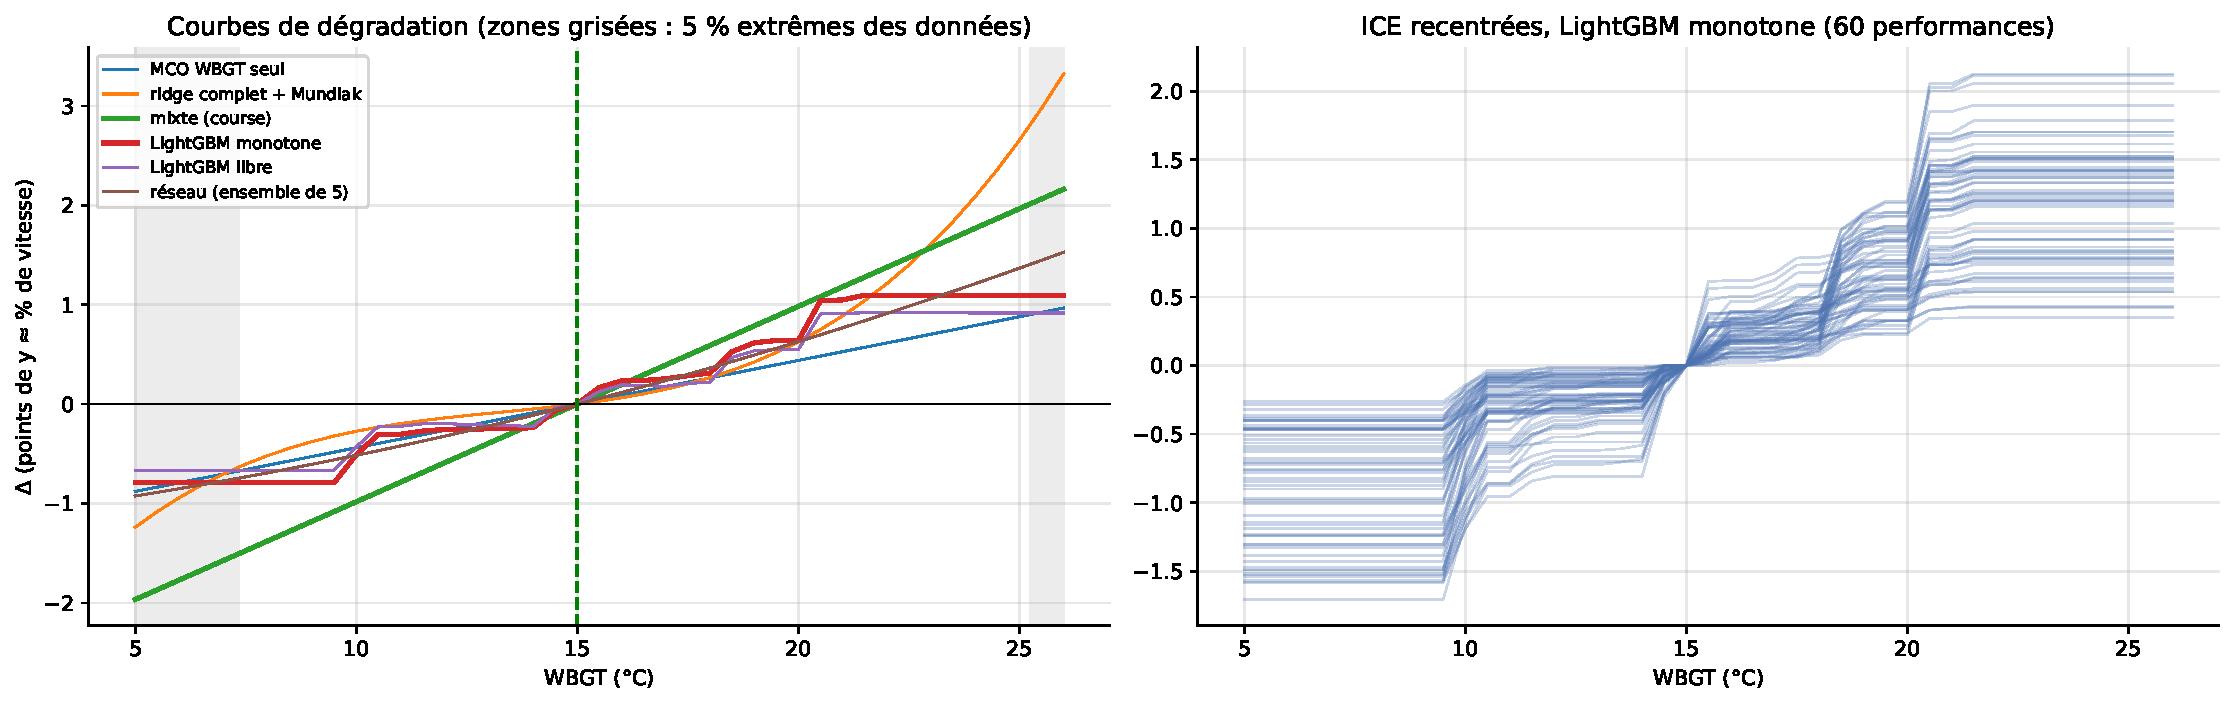
\includegraphics[width=\textwidth]{courbes_modeles}
\caption{À gauche, courbes de dégradation $\Delta(W)$ de six modèles, moyennées sur les performances d'apprentissage,
toutes épreuves confondues ; les zones grisées couvrent les 2,5~\% extrêmes des données de chaque côté. À droite,
courbes ICE recentrées du boosting monotone pour 60 performances tirées au hasard.}
\label{fig:courbes_modeles}
\end{figure}

Les courbes de dégradation des six modèles ont toutes le même sens : plus chaud, plus lent
(figure~\ref{fig:courbes_modeles}). Mais leur amplitude et leur forme diffèrent nettement au-delà de 20~°C. À 25~°C, la
dégradation vaut environ $+0{,}9$~point pour les moindres carrés sur le WBGT seul, qui ne contrôlent aucun facteur
confondant ; $+1{,}1$ pour les deux boostings, dont la courbe en marches devient constante au-delà de 21~°C environ ;
$+1{,}4$ pour l'ensemble de réseaux, dont la courbe est lisse et presque linéaire ; $+1{,}9$ pour le modèle mixte,
dont la courbe est une droite ; et $+2{,}6$ pour le ridge complet, dont le polynôme de degré~3 est convexe. Les arbres
plafonnent : au-delà du dernier seuil appris sur le WBGT, faute de courses chaudes en nombre suffisant, ils prédisent la
même chose quel que soit le WBGT. Le polynôme de degré~3, à l'inverse, s'envole : sa courbure est portée par les
quelques courses les plus chaudes, et dépasse 3~points dans la zone grisée, où les données manquent. Côté frais, tous
les modèles prédisent une performance plus rapide qu'à 15~°C, avec un écart entre eux qui se creuse sous 7,5~°C, de
$-0{,}8$ à $-1{,}9$~point à 5~°C. Les courbes ICE du boosting, enfin, sont loin d'être parallèles : à 25~°C, la
dégradation va d'environ $+0{,}4$ à $+2{,}1$~points selon la performance. L'effet de la chaleur dépend donc des autres
variables, épreuve, durée ou heure, ce qui justifie d'estimer un effet par groupe d'épreuves. Les marches, situées vers
10, 14,5, 18,5 et 20,5~°C, sont les seuils de coupure des arbres, communs à toutes les performances.

Nous étions donc face à un constat embarrassant : cinq modèles de précision indiscernable donnent, pour une hausse de
10~°C, des effets allant du simple au triple. La précision prédictive ne permet pas de choisir entre eux ; c'est la
forme qu'ils imposent ou n'imposent pas à la courbe qui fait la différence. Il fallait choisir le modèle de l'outil
sur d'autres critères, et mesurer l'incertitude de sa courbe.

\subsection{Incertitude sur la courbe : le bootstrap des lieux}\label{sec:bootstrap_courbe}

Pour l'outil, les modèles sont désormais réentraînés sur tous les lieux, apprentissage et test réunis. Le test a déjà
servi à l'évaluation, et il n'y a plus aucun choix à faire en le regardant : l'utiliser pour estimer l'effet ne crée
aucune fuite, et 21 lieux de plus améliorent la précision.

L'incertitude sur $\Delta(W)$ vient surtout du petit nombre de lieux et de courses : chaque course n'apporte qu'une
situation météorologique, et les courses chaudes sont rares. Nous l'estimons par un bootstrap des lieux, mais cette
fois en réentraînant le modèle sur chaque réplique. On tire avec remise autant de lieux qu'il y en a dans les données,
on réunit toutes leurs performances et l'on réentraîne le modèle sur cet échantillon, puis on calcule la courbe de
dégradation du modèle réentraîné sur une population de référence fixe ; après $B$ répétitions, on prend, point par
point de la grille, les quantiles d'ordre 0,025 et 0,975 des $B$ courbes. On obtient une bande de confiance
\emph{ponctuelle} à 95~\% : pour chaque valeur de WBGT, l'intervalle contient la vraie valeur de la courbe avec une
probabilité d'environ 95~\%. Ce n'est pas une bande \emph{simultanée}, et la probabilité que la courbe entière reste
dans la bande est plus faible. Ce bootstrap mesure l'incertitude due à l'échantillon de lieux, y compris la variabilité
de l'estimation de tous les coefficients, mais pas celle due à un mauvais choix de forme du modèle.

Deux précautions sont essentielles. La courbe est toujours calculée sur la même population de référence, et non sur
l'échantillon bootstrap, dont la composition change à chaque réplique : sinon, la variabilité mesurée mélangerait
celle du modèle et celle de la population sur laquelle on moyenne. Et chaque copie d'un lieu tiré plusieurs fois doit
devenir un lieu distinct, avec ses propres courses. Sans cette précaution, les courses d'un lieu tiré deux fois
deviendraient des courses de taille double, faites de paires de lignes identiques : un modèle mixte y verrait une
variance intra-course artificiellement faible et pourrait estimer $\gamma \to \infty$, avec des effets aberrants. Dans
la logique du bootstrap, chaque tirage représente d'ailleurs un nouveau lieu de la population.

\subsection{Le modèle retenu pour l'outil}\label{sec:modele_outil}

Pour l'outil, ce qui compte est l'effet des conditions : estimé avec le moins de biais possible, assorti d'une
incertitude honnête, lisible par épreuve, et sans extrapolation fantaisiste. Nous avons retenu un modèle linéaire à
intercept aléatoire de course, dont les termes sont choisis a priori d'après la physiologie et la littérature. Pour la
performance $j$ de la course $g$,
\begin{multline}\label{eq:modele_outil}
y_{gj} = u_g + \sum_e \mathbb 1_e\,P_e(W_{gj}) + \beta_{W,\text{niv}}\,\frac{\text{niveau}_{gj}}{10}\,(W_{gj} - W_{\text{ref}})
+ \sum_e \mathbb 1_e\,\beta_{\text{alt},e}\,\text{alt}_g \\
+ \beta_{\text{vent}}\,\text{vent}_{gj} + \beta_{\text{pluie}}\,\text{pluie}_{gj} + x_{gj}^\top\beta + \varepsilon_{gj},
\end{multline}
avec $u_g \sim \mathcal N(0, \tau^2)$ et $\varepsilon_{gj} \sim \mathcal N(0, \sigma^2)$. Le terme $P_e$ est un
polynôme du WBGT propre à chaque groupe d'épreuves $e$, et $\mathbb 1_e$ vaut 1 pour les performances du groupe $e$ :
l'effet de la chaleur peut ainsi croître avec la durée de l'effort. Les polynômes s'écrivent dans la base $\psi(W)$,
nulle en $W_{\text{ref}}$, et leur degré est choisi par validation croisée par lieux. Le terme $\beta_{W,\text{niv}}$
multiplie l'écart de WBGT à la référence par le niveau de l'athlète, en dizaines de points : il teste le résultat de
\citet{ely2007}, selon lequel les coureurs lents sont plus affectés par la chaleur. L'altitude au-delà de 500~m,
$\text{alt}_g$, a une pente propre à chaque groupe ; les pistes de nos données étant toutes sous 300~m, son
coefficient est nul pour les deux groupes de piste, et l'outil refusera toute altitude supérieure à celle observée
pour le groupe. Les contrôles $x_{gj}$ regroupent l'âge, la forme, l'heure, la durée attendue, le niveau, le sexe et le
groupe d'épreuves. Nous n'avons pas inclus de terme de Mundlak : avec un effet propre à chaque groupe, il faudrait une
moyenne de parcours par groupe, et nous avons vu que l'effet intra-parcours n'est pas plus faible que l'effet estimé
sans distinction.

Ce choix écarte les deux autres candidats sérieux. La courbe du boosting monotone est contrainte à être croissante :
si l'effet réel est nul, elle est biaisée vers le haut, et son intervalle bootstrap ne peut pas contenir de valeurs
négatives au-dessus de la référence ; elle est aussi en marches, et plafonne au-delà des derniers seuils appris. La
courbe du réseau est lisse, mais elle ne se décompose pas par épreuve, et son incertitude demanderait de réentraîner
des ensembles de réseaux des centaines de fois. Le modèle linéaire mixte donne une courbe lisse, propre à chaque
épreuve, dont chaque terme a une interprétation et un intervalle de confiance.

La validation croisée par lieux donne une RMSE de 3,024 pour un effet linéaire du WBGT dans chaque groupe, 3,028 en
degré~2 et 3,042 en degré~3 : le degré~1 est retenu, les données ne permettant pas d'estimer une courbure propre à
chaque groupe, et la règle d'un écart-type aurait fait le même choix.

\paragraph{Une difficulté inattendue : la vraisemblance REML est bimodale.} En estimant ce modèle, nous avons constaté
que la log-vraisemblance restreinte profilée $\ell_R(\gamma)$ n'a pas toujours un seul maximum. Outre le maximum
intérieur, elle peut remonter vers la borne $\gamma \to \infty$, qui correspond aux effets fixes de course
(figure~\ref{fig:profil_reml}). La cause principale est l'hétéroscédasticité : l'écart-type de $y$ au sein d'une
course vaut environ 1,9~point en demi-fond et 3,6 au marathon, alors que le modèle suppose un $\sigma^2$ commun. En
traitant chaque course comme un effet fixe, le modèle absorbe une partie de cette hétérogénéité dans les moyennes de
course, ce que la vraisemblance peut récompenser. Sur l'échantillon complet, le maximum intérieur est atteint en
$\ln\hat\gamma = -2{,}12$, soit $\hat\gamma = 0{,}120$, avec $\hat\tau^2 = 0{,}945$ et $\hat\sigma^2 = 7{,}873$ : la
course explique 11~\% de la variance résiduelle. La vraisemblance descend ensuite jusqu'à environ $-16\,585$ vers
$\ln\gamma \approx 2{,}8$, puis remonte jusqu'à $-16\,396$ à la borne $\ln\gamma = 6$ ; le maximum intérieur
($-16\,192$) l'emporte de plus de 200 unités de log-vraisemblance. Mais dans une réplique bootstrap, la borne pourrait
l'emporter : les variables de niveau course (WBGT, altitude, groupe d'épreuves) ne seraient alors plus identifiées que
par l'infime variation qui subsiste au sein des courses, et leurs effets deviendraient aberrants.

\begin{figure}[htbp]
\centering
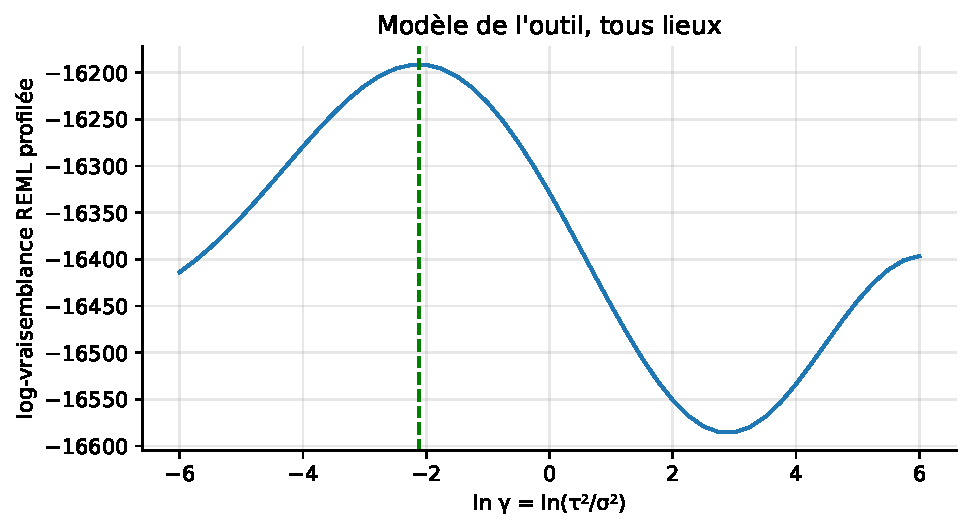
\includegraphics[width=0.6\textwidth]{profil_reml}
\caption{Log-vraisemblance restreinte profilée du modèle de l'outil, estimé sur tous les lieux, en fonction de
$\ln\gamma$. La ligne pointillée marque le maximum intérieur, en $\ln\hat\gamma = -2{,}12$ ; la remontée vers la borne
droite correspond aux effets fixes de course.}
\label{fig:profil_reml}
\end{figure}

Nous avons résolu cette difficulté en fixant $\gamma$ à sa valeur estimée sur l'échantillon complet, $\hat\gamma$, dans
toutes les répliques. Chaque réplique calcule alors un estimateur des moindres carrés généralisés avec une matrice de
covariance \emph{de travail} $V = V(\hat\gamma)$ fixée, $\hat\beta = (X^\top V^{-1} X)^{-1} X^\top V^{-1} y$. Cet
estimateur reste sans biais même si $V$ n'est pas la vraie covariance : comme $\E[y] = X\beta$,
\[
\E[\hat\beta] = (X^\top V^{-1} X)^{-1} X^\top V^{-1} X\beta = \beta,
\]
quelle que soit la matrice $V$ utilisée. Une matrice imparfaite ne coûte que de la précision. Sa variance n'est en
revanche plus celle que donnerait la formule du modèle : si la vraie covariance est $\Sigma$, elle vaut
\[
\Var(\hat\beta) = (X^\top V^{-1} X)^{-1}\,X^\top V^{-1}\,\Sigma\,V^{-1} X\,(X^\top V^{-1} X)^{-1},
\]
la variance dite « sandwich », celle des équations d'estimation généralisées \citep{liang1986}. Le bootstrap des lieux
estime cette variance sans avoir à connaître $\Sigma$ : l'incertitude obtenue est robuste à une covariance mal
spécifiée. Une alternative plus complète aurait consisté à estimer un $\sigma^2$ propre à chaque groupe d'épreuves.

\paragraph{L'effet de la chaleur par groupe d'épreuves.} La dégradation $\Delta(W)$ est calculée séparément sur les
performances de référence de chaque groupe, avec un intervalle obtenu par 300 répliques bootstrap
(tableau~\ref{tab:effets} et figure~\ref{fig:courbes_finales}). Les valeurs situées au-delà du centile 99 du WBGT
observé pour le groupe sont signalées comme des extrapolations.

\begin{table}[htbp]
\centering
\small
\caption{Dégradation $\Delta$ estimée par le modèle de l'outil depuis un WBGT de 15~°C, en points de $y$
(approximativement en pourcentage de vitesse), avec intervalles de confiance à 95~\% par bootstrap des lieux
(300 répliques).}
\label{tab:effets}
\begin{tabular}{@{}lcc@{}}
\toprule
Groupe d'épreuves & WBGT de 20~°C & WBGT de 25~°C \\
\midrule
demi-fond piste & $+0{,}02$ \ [$-0{,}43$ ; $+0{,}35$] & $+0{,}04$ \ [$-0{,}86$ ; $+0{,}69$] \\
fond piste & $+0{,}41$ \ [$-0{,}01$ ; $+1{,}08$] & $+0{,}82$ \ [$-0{,}02$ ; $+2{,}17$] \\
route courte & $+0{,}76$ \ [$+0{,}24$ ; $+1{,}25$] & $+1{,}52$ \ [$+0{,}48$ ; $+2{,}51$] \\
semi-marathon & $+0{,}89$ \ [$+0{,}47$ ; $+1{,}34$] & $+1{,}78$ \ [$+0{,}93$ ; $+2{,}68$] \ (extrapolé) \\
marathon & $+1{,}57$ \ [$+1{,}16$ ; $+2{,}06$] & $+3{,}14$ \ [$+2{,}32$ ; $+4{,}12$] \\
\bottomrule
\end{tabular}
\end{table}

\begin{figure}[htbp]
\centering
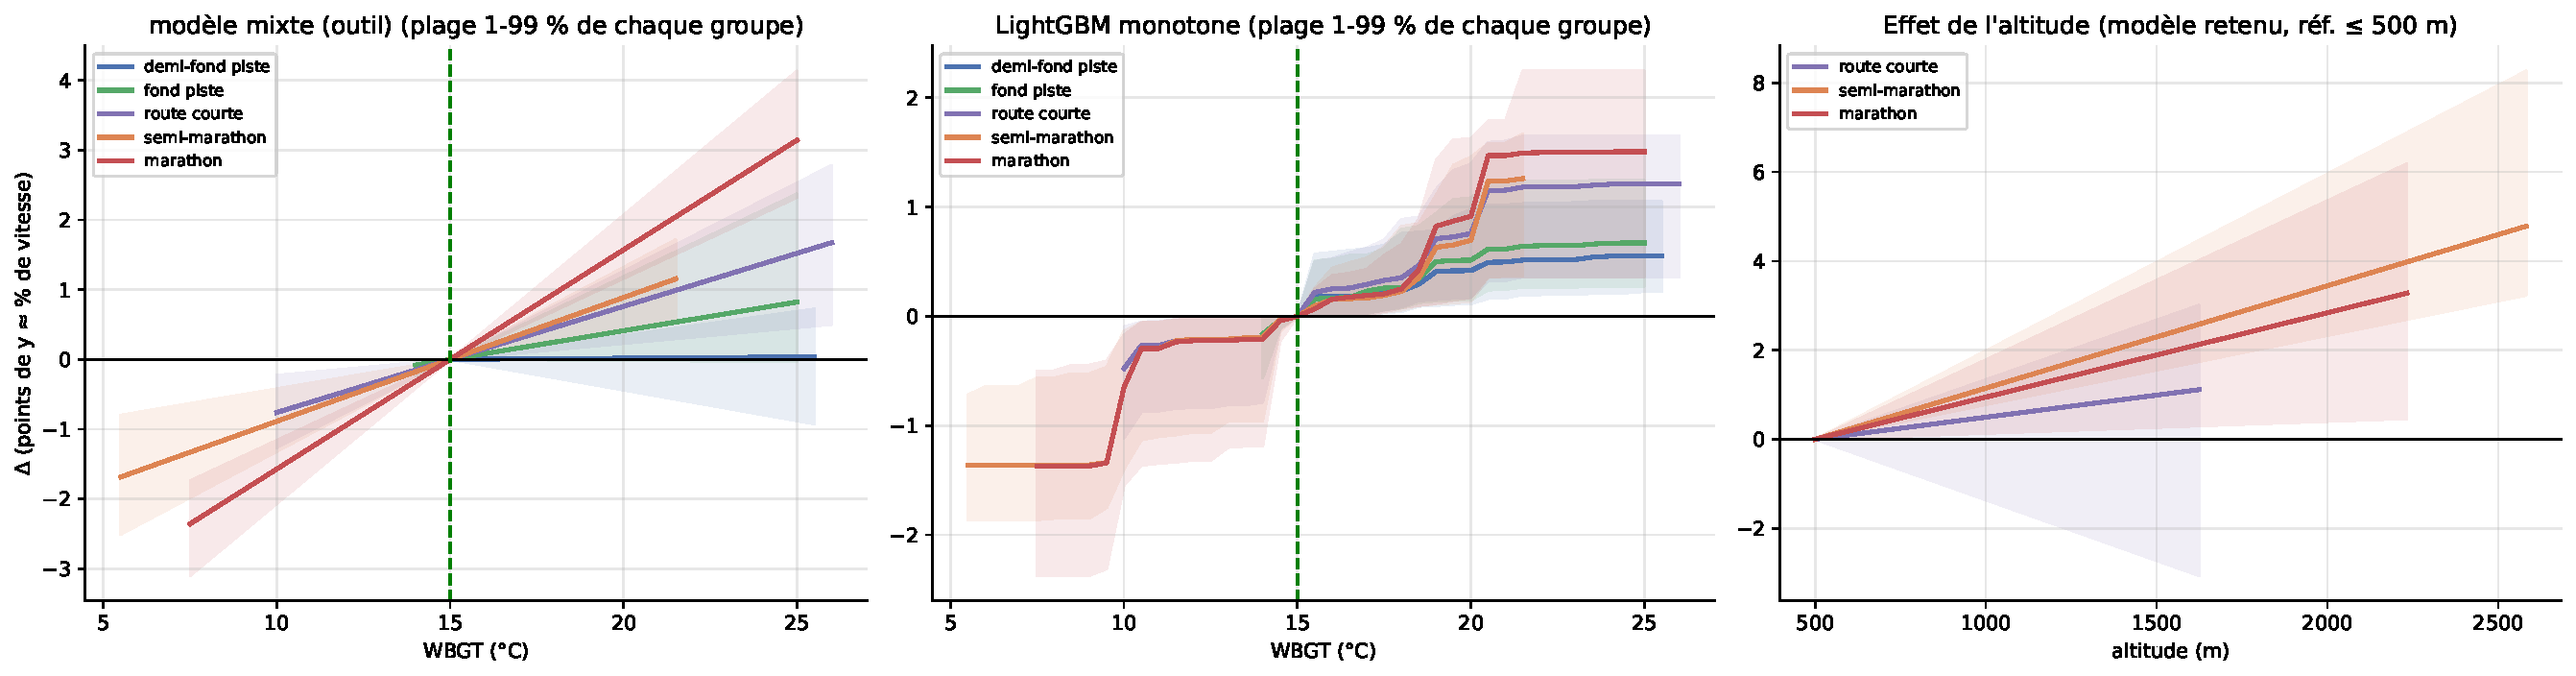
\includegraphics[width=\textwidth]{courbes_finales}
\caption{Courbes de dégradation par groupe d'épreuves, sur la plage des centiles 1 à 99 du WBGT de chaque groupe,
avec bandes de confiance ponctuelles à 95~\% par bootstrap des lieux : modèle de l'outil (à gauche, 300 répliques) et
boosting monotone (au centre, 50 répliques). À droite, effet de l'altitude estimé par le modèle de l'outil, par
rapport à une altitude inférieure à 500~m.}
\label{fig:courbes_finales}
\end{figure}

L'effet croît avec la durée de l'effort, comme le prévoit la physiologie : la chaleur stockée s'accumule et la dérive
cardiovasculaire s'installe au fil de l'effort. Il est nul en demi-fond, où un 800~m ou un 1\,500~m est trop court pour
que la thermorégulation limite la performance ; l'intervalle, centré sur 0, exclut un effet supérieur à 0,7~point à
25~°C. Il vaut environ 0,8~point en fond sur piste, avec un intervalle qui touche 0, puis environ 1,5~point sur route
courte. Il atteint environ 3~points au marathon entre 15 et 25~°C, soit environ 4~min~45~s sur un marathon couru en
2~h~30, l'ordre de grandeur rapporté par \citet{ely2007}. Le semi-marathon à 25~°C est une extrapolation, aucune course
n'ayant été observée au-delà de 22~°C. Les effets étant linéaires, celui de 25~°C est le double de celui de 20~°C ; or
les moyennes par classes suggéraient une accélération au-delà de 20~°C au marathon, si bien que le modèle peut
sous-estimer légèrement l'effet vers 25~°C et le surestimer vers 18 à 20~°C. Pondéré par les effectifs des groupes,
l'effet d'une hausse de 10~°C vaut environ 1,7~point, un peu moins que les estimations de la
section~\ref{sec:quel_estimateur} (1,9 à 2,4~points), obtenues sur les seuls lieux d'apprentissage avec un effet commun
à toutes les épreuves, mais du même ordre de grandeur.

Les autres termes complètent le tableau. Le vent coûte $0{,}36$~point pour 2~m/s de plus à 10~m (intervalle
$[0{,}08\,;\,0{,}63]$), à WBGT égal : son effet rafraîchissant passe déjà par le WBGT, et il reste l'effet mécanique,
le vent de face n'étant pas compensé par le vent de dos. La pluie, trop rare, ne permet pas de conclure ($+0{,}34$ pour
1~mm/h, intervalle $[-0{,}53\,;\,2{,}00]$). L'écart entre coureurs lents et rapides prédit par \citet{ely2007} n'est
pas détecté au marathon : pour une hausse de 10~°C, un coureur de niveau $+10$ perd $0{,}17$~point de moins qu'un
coureur de niveau $-10$, avec un intervalle $[-1{,}24\,;\,0{,}86]$ ; nos données ne contiennent que de bons coureurs,
sur une plage de niveaux étroite. L'altitude, enfin, coûte à 1\,500~m environ 1,9~point au marathon (intervalle
$[0{,}05\,;\,3{,}65]$) et 2,3~points au semi-marathon ($[1{,}55\,;\,4{,}48]$), et reste indéterminée sur route courte
($+0{,}99$, intervalle $[-2{,}95\,;\,2{,}80]$). Ces effets reposent sur 3 à 6 lieux par groupe, d'où la largeur des
intervalles, et peuvent aussi refléter les parcours propres à ces villes.

Le boosting monotone, gardé comme point de comparaison, donne le même classement des épreuves et des valeurs proches
jusqu'à 20~°C, mais il plafonne au-delà : environ $+1{,}5$~point au marathon à 25~°C, contre 3,1 pour le modèle mixte.
La contrainte de monotonie a un autre effet, visible en demi-fond : sa courbe ne peut pas descendre sous 0 au-dessus de
15~°C, et monte jusqu'à environ $+0{,}5$~point avec un intervalle qui exclut 0, alors que le modèle mixte trouve un
effet nul. C'est le biais annoncé : quand l'effet réel est nul, une courbe contrainte à monter ne peut que le
surestimer. Les deux modèles s'accordent en revanche côté frais : au marathon, courir à 7 ou 8~°C plutôt qu'à 15~°C
fait gagner de 1,4 à 2,4~points.

\section{L'incertitude de prédiction}\label{sec:incertitude}

Deux incertitudes ne doivent pas être confondues. L'\emph{intervalle de confiance} porte sur un paramètre ou un effet
moyen, ici la courbe de dégradation $\Delta(W)$ : il traduit l'imprécision due à la taille finie de l'échantillon, et
se resserrerait jusqu'à zéro avec plus de lieux et de courses. L'\emph{intervalle de prédiction}
$\hat I(x) = [\hat q_{\text{bas}}(x)\,;\,\hat q_{\text{haut}}(x)]$ porte sur une observation future : il doit contenir
la performance $y$ d'un athlète avec une probabilité $1 - \alpha$. Même avec un modèle parfait, connu sans erreur, il
reste aussi large que le bruit individuel, et ne se resserre pas avec les données. Un outil honnête doit pouvoir dire
les deux ; nous avons cherché à construire des intervalles de prédiction à 90~\% ($\alpha = 0{,}1$).

\subsection{Régression quantile et perte pinball}\label{sec:pinball}

La moyenne minimise la perte quadratique et la médiane la perte absolue. Plus généralement, le quantile d'ordre
$\alpha$ d'une variable $Y$, la valeur $q$ telle que $\mathbb{P}(Y \leq q) = \alpha$, minimise l'espérance de la
\emph{perte pinball}
\[
\rho_\alpha(y, q) = \max\big(\alpha\,(y - q),\ (\alpha - 1)(y - q)\big) =
\begin{cases} \alpha\,(y - q) & \text{si } y \geq q, \\ (1 - \alpha)\,(q - y) & \text{si } y < q. \end{cases}
\]
En effet, pour une variable $Y$ de fonction de répartition $F$ continue,
\[
\E[\rho_\alpha(Y, q)] = \alpha\int_{q}^{+\infty}(y - q)\,\dd F(y) + (1 - \alpha)\int_{-\infty}^{q}(q - y)\,\dd F(y),
\]
dont la dérivée en $q$ vaut $-\alpha\,\big(1 - F(q)\big) + (1 - \alpha)\,F(q) = F(q) - \alpha$. Elle s'annule quand
$F(q) = \alpha$, et la fonction est convexe : le minimum est atteint au quantile d'ordre $\alpha$. Une prédiction trop
basse coûte $\alpha$ par unité et une prédiction trop haute $1 - \alpha$ : pour $\alpha = 0{,}95$, être trop bas coûte
19 fois plus qu'être trop haut, et l'on place $q$ assez haut pour que 95~\% des observations soient en dessous. Pour
$\alpha = 0{,}5$, on retrouve la perte absolue et la médiane.

En minimisant la perte pinball moyenne sur les données au lieu de l'erreur quadratique, un modèle estime un quantile
conditionnel $\hat q_\alpha(x)$ : c'est la \emph{régression quantile} \citep{koenker1978}. Deux boostings, pour les
ordres $0{,}05$ et $0{,}95$, donnent un intervalle de prédiction « brut » à 90~\%, dont la largeur s'adapte à $x$. Rien
ne garantit cependant sa couverture : appris sur les données d'apprentissage, ces quantiles ignorent l'erreur
d'estimation du modèle lui-même et la différence entre les lieux d'apprentissage et un lieu nouveau.

\subsection{La prédiction conforme}\label{sec:conforme}

La \emph{prédiction conforme} \citep{vovk2005} corrige ce défaut en calibrant l'intervalle sur un ensemble séparé de
$n$ observations, non utilisées pour l'apprentissage. On calcule sur cet ensemble un \emph{score de non-conformité}
$s_i$, d'autant plus grand que l'observation $i$ est mal prédite, puis le seuil $\hat q$, égal à la
$\lceil (n+1)(1-\alpha)\rceil$-ième plus petite valeur des scores (et $+\infty$ si cet indice dépasse $n$). On retient
comme intervalle de prédiction l'ensemble des valeurs $y$ dont le score serait inférieur ou égal à $\hat q$.

La garantie repose sur une seule hypothèse : les scores des $n$ observations de calibration et celui d'une nouvelle
observation sont \emph{échangeables}, c'est-à-dire que leur loi jointe est inchangée quand on les permute. C'est le cas
s'ils sont indépendants et de même loi, mais l'hypothèse est plus faible. Sous cette hypothèse, et en l'absence
d'égalités, le rang du nouveau score parmi les $n + 1$ scores est uniforme sur $\{1, \dots, n + 1\}$ : le nouveau
score est donc inférieur ou égal à la $k$-ième plus petite valeur de calibration avec une probabilité d'au moins
$k/(n + 1)$. Avec $k = \lceil (n+1)(1-\alpha)\rceil$, on obtient
\begin{equation}\label{eq:garantie_conforme}
\mathbb{P}\big(y \in \hat I(x)\big) \geq \frac{\lceil (n+1)(1-\alpha)\rceil}{n + 1} \geq 1 - \alpha .
\end{equation}
La garantie vaut en échantillon fini, quelle que soit la qualité du modèle et sans aucune hypothèse sur la loi des
données : un mauvais modèle donne des intervalles larges, mais toujours bien calibrés. La correction $n + 1$ compte, le
quantile empirique ordinaire sous-couvrant légèrement, surtout pour un petit ensemble de calibration.

Nous avons comparé deux scores. Le score conforme simple, $s_i = |y_i - \hat y(x_i)|$, est l'erreur absolue d'un
modèle de la moyenne ; l'intervalle $\hat y(x) \pm \hat q$ est de largeur constante, aussi large pour un 800~m que
pour un marathon. La régression quantile conformalisée \citep[CQR,][]{romano2019} part au contraire des quantiles
bruts, avec le score $s_i = \max\big(\hat q_{\text{bas}}(x_i) - y_i,\ y_i - \hat q_{\text{haut}}(x_i)\big)$, qui mesure
de combien $y_i$ dépasse l'intervalle brut et qui est négatif si $y_i$ est à l'intérieur. L'intervalle
$[\hat q_{\text{bas}}(x) - \hat q\,;\,\hat q_{\text{haut}}(x) + \hat q]$ garde la largeur adaptative des quantiles
bruts, élargie, ou rétrécie si $\hat q < 0$, juste assez pour atteindre la couverture voulue. Dans les deux cas, la
garantie est \emph{marginale} : elle porte sur la proportion de performances couvertes en moyenne, et ne garantit pas
la couverture \emph{conditionnelle} à un sous-groupe, comme les marathons. Certains groupes peuvent être sur-couverts et
d'autres sous-couverts, la moyenne restant correcte.

Nous avons entraîné trois boostings, la moyenne avec contrainte de monotonie et les quantiles d'ordres $0{,}05$ et
$0{,}95$, sur quatre plis de lieux, calibré sur le cinquième pli, et évalué sur les lieux de test. Calibrer sur des
lieux que le modèle n'a pas vus devait reproduire la situation d'un lieu nouveau. L'échangeabilité n'est cependant
qu'approchée : calibration et test portent sur des lieux différents, et les performances d'une même course sont
corrélées.

\subsection{Une garantie qui ne tient pas, et pourquoi}\label{sec:sous_couverture}

Sur les lieux de test, les quantiles bruts couvrent 86,8~\% des performances, pour une largeur moyenne de
8,13~points. L'intervalle conforme simple ($\hat q = 3{,}655$) couvre 83,4~\% pour une largeur de 7,31, et la CQR
($\hat q = -0{,}211$) 84,2~\% pour une largeur de 7,71. Les pertes pinball sur le test valent 0,242 pour le quantile
d'ordre 0,05 et 0,355 pour celui d'ordre 0,95. Les intervalles calibrés sous-couvrent donc : ils ne couvrent que 83 à
84~\% des performances au lieu des 90~\% garantis, et font même moins bien que les quantiles bruts.

La garantie \eqref{eq:garantie_conforme} n'est pas fausse : c'est son hypothèse qui n'est pas satisfaite. Le pli de
calibration est le pli~0, le plus facile des cinq : le modèle constant y obtenait une RMSE de 2,65, contre 3,19 sur les
lieux de test. Ses performances, moins dispersées, donnent des scores plus petits que ceux des lieux de test : les
scores de calibration et de test ne sont pas échangeables, le seuil $\hat q$ est trop petit et l'intervalle trop
étroit. Le signe du seuil de la CQR le montre bien : $\hat q$ est négatif, ce qui signifie que, sur le pli de
calibration, les quantiles bruts semblaient trop larges, et la CQR les a rétrécis alors qu'ils étaient déjà un peu
trop étroits pour les lieux de test. Une garantie conforme ne vaut que si l'ensemble de calibration est représentatif
des données sur lesquelles on l'applique. Avec des données groupées par lieux, très hétérogènes d'un lieu à l'autre,
un pli de 14 lieux ne suffit pas à représenter la variabilité entre lieux. Deux remèdes sont possibles : calibrer sur
plusieurs plis, en utilisant les prédictions hors pli de la validation croisée, ou calibrer par groupe d'épreuves.

La CQR adapte bien la largeur à l'épreuve : 5,0~points en demi-fond, 6,3 en fond sur piste, 8,4 sur route courte, 9,7
au semi-marathon et 10,4 au marathon, ce qui reflète l'hétéroscédasticité observée dès l'exploration. Sa couverture
varie pourtant de 79,6~\% en demi-fond à 88,6~\% au semi-marathon, avec 86,8~\% en fond sur piste, 85,1~\% sur route
courte et 85,8~\% au marathon : la garantie, déjà approchée en moyenne, ne vaut pas groupe par groupe.

Ces intervalles de prédiction, d'environ $\pm 4$~points, sont bien plus larges que l'intervalle de confiance de la
courbe de dégradation, de $\pm 0{,}4$ à $\pm 1$~point. Le premier porte sur le chrono d'une performance individuelle et
inclut la forme du jour, la tactique et l'ancienneté du record, un bruit d'écart-type proche de 2,8~points qui ne
diminue pas avec la taille de l'échantillon ; le second porte sur l'effet moyen des conditions, qui se précise avec les
données. Pour régler une allure, c'est $\Delta$ et son intervalle de confiance qui comptent : la question est « de
combien ralentir pour fournir le même effort », et non « quel chrono vais-je faire ». La borne haute de l'intervalle de
confiance donne une allure prudente. L'intervalle de prédiction rappelle, lui, qu'un chrono individuel reste très
incertain, quelles que soient les conditions.

\section{L'outil : la vitesse à effort égal}\label{sec:outil}

\subsection{Du modèle à la vitesse équivalente}\label{sec:conversion}

L'outil reçoit la vitesse $Y$ visée en conditions de référence, les conditions du jour $\mathcal{C}$ (température,
humidité, vent à 10~m, rayonnement global, pluie, altitude, ainsi que la date, l'heure et le lieu, qui fixent la
position du soleil), l'épreuve et le sexe. Les conditions de référence $\mathcal{C}_{\text{ref}}$ sont un WBGT de
15~°C, un vent de 2~m/s à 10~m, l'absence de pluie et une altitude d'au plus 500~m. Le calcul suit cinq étapes.

Le WBGT du jour est d'abord calculé par le modèle de Liljegren. La pression est déduite de l'altitude $z$, en mètres,
par la formule barométrique de l'atmosphère standard,
\[
p(z) = 1013{,}25\,\big(1 - 2{,}2557\cdot 10^{-5}\,z\big)^{5{,}2559}\ \text{hPa},
\]
qui découle de l'équilibre hydrostatique d'une atmosphère dont la température décroît linéairement avec l'altitude :
$2{,}2557\cdot10^{-5} = L/T_0$, avec un gradient thermique $L = 0{,}0065$~K/m et une température au sol
$T_0 = 288{,}15$~K, et $5{,}2559 = g_0 M/(R L)$, où $g_0$ est l'accélération de la pesanteur, $M$ la masse molaire de
l'air et $R$ la constante des gaz parfaits. À 1\,000~m, la pression est inférieure de 11~\% à celle du niveau de la
mer.

On construit ensuite le profil implicite de l'athlète. Sa vitesse $Y$ correspond, sur la distance $d$, à un temps
$t_Y = d/Y$, que l'on traite comme son record : son niveau vaut $100\ln(t_Y/t^{\RP}_{\text{méd}})$, où
$t^{\RP}_{\text{méd}}$ est le record médian du sexe et de l'épreuve, et sa durée attendue vaut $t_Y/60$ minutes.

La dégradation $\Delta = f(\mathcal{C}) - f(\mathcal{C}_{\text{ref}})$ est alors calculée sur un ensemble de
performances réelles de la même épreuve et du même sexe, jusqu'à 200 : on leur donne le profil de l'athlète, on impose
les conditions $\mathcal{C}$, puis les conditions de référence (WBGT, vent, pluie \emph{et} altitude), et l'on moyenne
la différence des prédictions. C'est une moyenne de courbes ICE, qui intègre sur les autres variables (âge, forme,
heure) observées pour ce type de course. Les conditions de référence doivent fixer toutes les variables
météorologiques : sinon, $\Delta$ mélangerait l'effet des conditions du jour et celui des conditions observées dans
la population de référence.

La vitesse équivalente est enfin $X = Y\,e^{-\Delta/100}$, d'après \eqref{eq:conversion}. Son intervalle de confiance
vient des 300 modèles bootstrap : avec $\Delta_{0{,}025}$ et $\Delta_{0{,}975}$ les quantiles des dégradations
bootstrap, $X_{\text{bas}} = Y\,e^{-\Delta_{0{,}975}/100}$ et $X_{\text{haut}} = Y\,e^{-\Delta_{0{,}025}/100}$. La
fonction $\Delta \mapsto Y e^{-\Delta/100}$ étant décroissante, la borne basse de la vitesse correspond à la borne haute
de la dégradation, et les quantiles se transportent sans approximation. L'approximation au premier ordre
$X \approx Y(1 - \Delta/100)$ serait d'autant moins bonne que $\Delta$ est grand, $\Delta$ étant exprimé en pourcents
logarithmiques.

La dernière étape est un garde-fou : si le WBGT du jour sort de la plage observée pour le groupe d'épreuves (entre ses
centiles 1 et 99), ou si l'altitude dépasse celle observée pour ce groupe, l'outil ne répond pas. Ces plages vont de
16,0 à 25,6~°C en demi-fond, de 13,5 à 25,2~°C en fond sur piste, de 9,8 à 27,4~°C sur route courte, de 5,2 à 21,8~°C
au semi-marathon et de 7,3 à 25,1~°C au marathon. Un modèle linéaire prolongerait docilement sa droite au-delà des
données ; nous avons préféré un outil qui ne répond pas à un outil qui répond faux.

\subsection{L'inversion : de la vitesse courue à la vitesse de référence}\label{sec:inversion}

Le problème inverse est le suivant : « j'ai couru à la vitesse $X$ dans les conditions $\mathcal{C}$ ; quelle vitesse
cela vaut-il en conditions de référence ? » Il s'agit de trouver la racine $Y$ de
\[
r(Y) = Y\,e^{-\Delta(\mathcal{C};\,Y)/100} - X .
\]
Comme $\Delta$ dépend de $Y$, par le niveau et la durée attendus de l'athlète, il n'y a pas de formule fermée, et nous
résolvons numériquement par la méthode de \citet{brent1973}. On encadre d'abord la racine, $r(0{,}8\,X) < 0 <
r(1{,}25\,X)$, puisque la dégradation reste de quelques pourcents. La dichotomie garantit alors la convergence : on
coupe l'intervalle en deux et l'on garde la moitié où $r$ change de signe, si bien que la largeur est divisée par deux
à chaque itération et qu'une précision de $10^{-7}$ est atteinte en une trentaine d'itérations. La méthode de Brent
combine cette sécurité avec deux méthodes plus rapides, la sécante, qui remplace $r$ par la droite passant par deux
points, et l'interpolation quadratique inverse, qui utilise une parabole passant par trois points. Elle utilise la
méthode rapide quand celle-ci fait progresser, et se replie sur la dichotomie sinon : la convergence est garantie dès
que $r(a)\,r(b) < 0$, et rapide quand $r$ est régulière.

\subsection{Quelques exemples}\label{sec:exemples}

Le calcul du WBGT a d'abord été contrôlé sur deux situations : 20~°C et 50~\% d'humidité à l'ombre donnent un WBGT de
15,2~°C, proche de la référence, et 30~°C, 70~\% d'humidité et un soleil de 600~W/m² donnent 31,0~°C, au-delà du
drapeau noir de l'ACSM. Un marathonien qui court à $Y = 4{,}80$~m/s en conditions de référence (2~h~26~min~30~s), par
22~°C et 60~\% d'humidité à l'ombre (WBGT de 18,1~°C), perd $\Delta = +0{,}93$~point : l'outil conseille
$X = 4{,}7554$~m/s, avec un intervalle de confiance de 4,7365 à 4,7734~m/s, et l'inversion retrouve exactement la
vitesse de départ, $Y = 4{,}80000$~m/s.

Prenons un marathonien de 2~h~30 en conditions de référence. Par temps frais, 15~°C à l'ombre et 70~\% d'humidité
(WBGT de 12,4~°C, sous la référence), l'outil lui conseille de courir plus vite : 2~h~28~min~49~s (intervalle de
2~h~28~min~17~s à 2~h~29~min~20~s). Par 22~°C, 70~\% d'humidité et un soleil de 300~W/m² (WBGT de 21,9~°C), son
marathon de référence en vaut 2~h~33~min~10~s, avec un intervalle de 2~h~31~min~47~s à 2~h~34~min~38~s. L'effet est
quasiment identique pour une marathonienne de 2~h~50 dans les mêmes conditions ($+2{,}12$~\%, soit 2~h~53~min~38~s) :
le modèle ne distingue pas les sexes dans l'effet de la chaleur. Par 27~°C et 80~\% au soleil, le WBGT (27,5~°C)
dépasse le centile 99 observé au marathon, et l'outil refuse de répondre. À 1\,500~m d'altitude et par 15~°C, le
marathon perd environ 1~\% (2~h~31~min~35~s), mais l'intervalle, de 2~h~28~min~44~s à 2~h~34~min~35~s, contient la
référence : l'effet de l'altitude reste très incertain. Sur 10~km, une coureuse de 35~min en référence en vaut
35~min~31~s par 25~°C, 75~\% d'humidité et 300~W/m² (WBGT de 25,2~°C). Sur piste, enfin, même par 28~°C (WBGT de
22,4~°C), l'allure ne change pas : un 1\,500~m en 3~min~50~s reste à 3~min~50~s, avec un intervalle qui ne dépasse pas
une ou deux secondes de part et d'autre.

\subsection{Un abaque température--humidité}\label{sec:abaque}

Un coureur raisonne en température et en humidité, pas en WBGT. L'abaque traduit l'outil dans ces termes : pour une
épreuve, un sexe, une vitesse de référence, un vent et un rayonnement donnés, on calcule le WBGT sur une grille de
températures (5 à 40~°C) et d'humidités (10 à 100~\%), puis la dégradation $\Delta$ dans chaque case. À vent, pluie et
altitude fixés, le modèle ne dépend de la météo qu'à travers le WBGT : il suffit donc d'évaluer $\Delta$ et ses
quantiles bootstrap sur une grille de valeurs de WBGT couvrant la plage du groupe, puis d'interpoler pour chaque case.
Chaque situation est représentée par deux panneaux : l'estimation centrale de $\Delta$, et la borne haute de son
intervalle de confiance à 95~\%, c'est-à-dire le ralentissement le plus fort compatible avec les données, la borne
prudente pour fixer une allure (figure~\ref{fig:abaque}).

\begin{figure}[htbp]
\centering
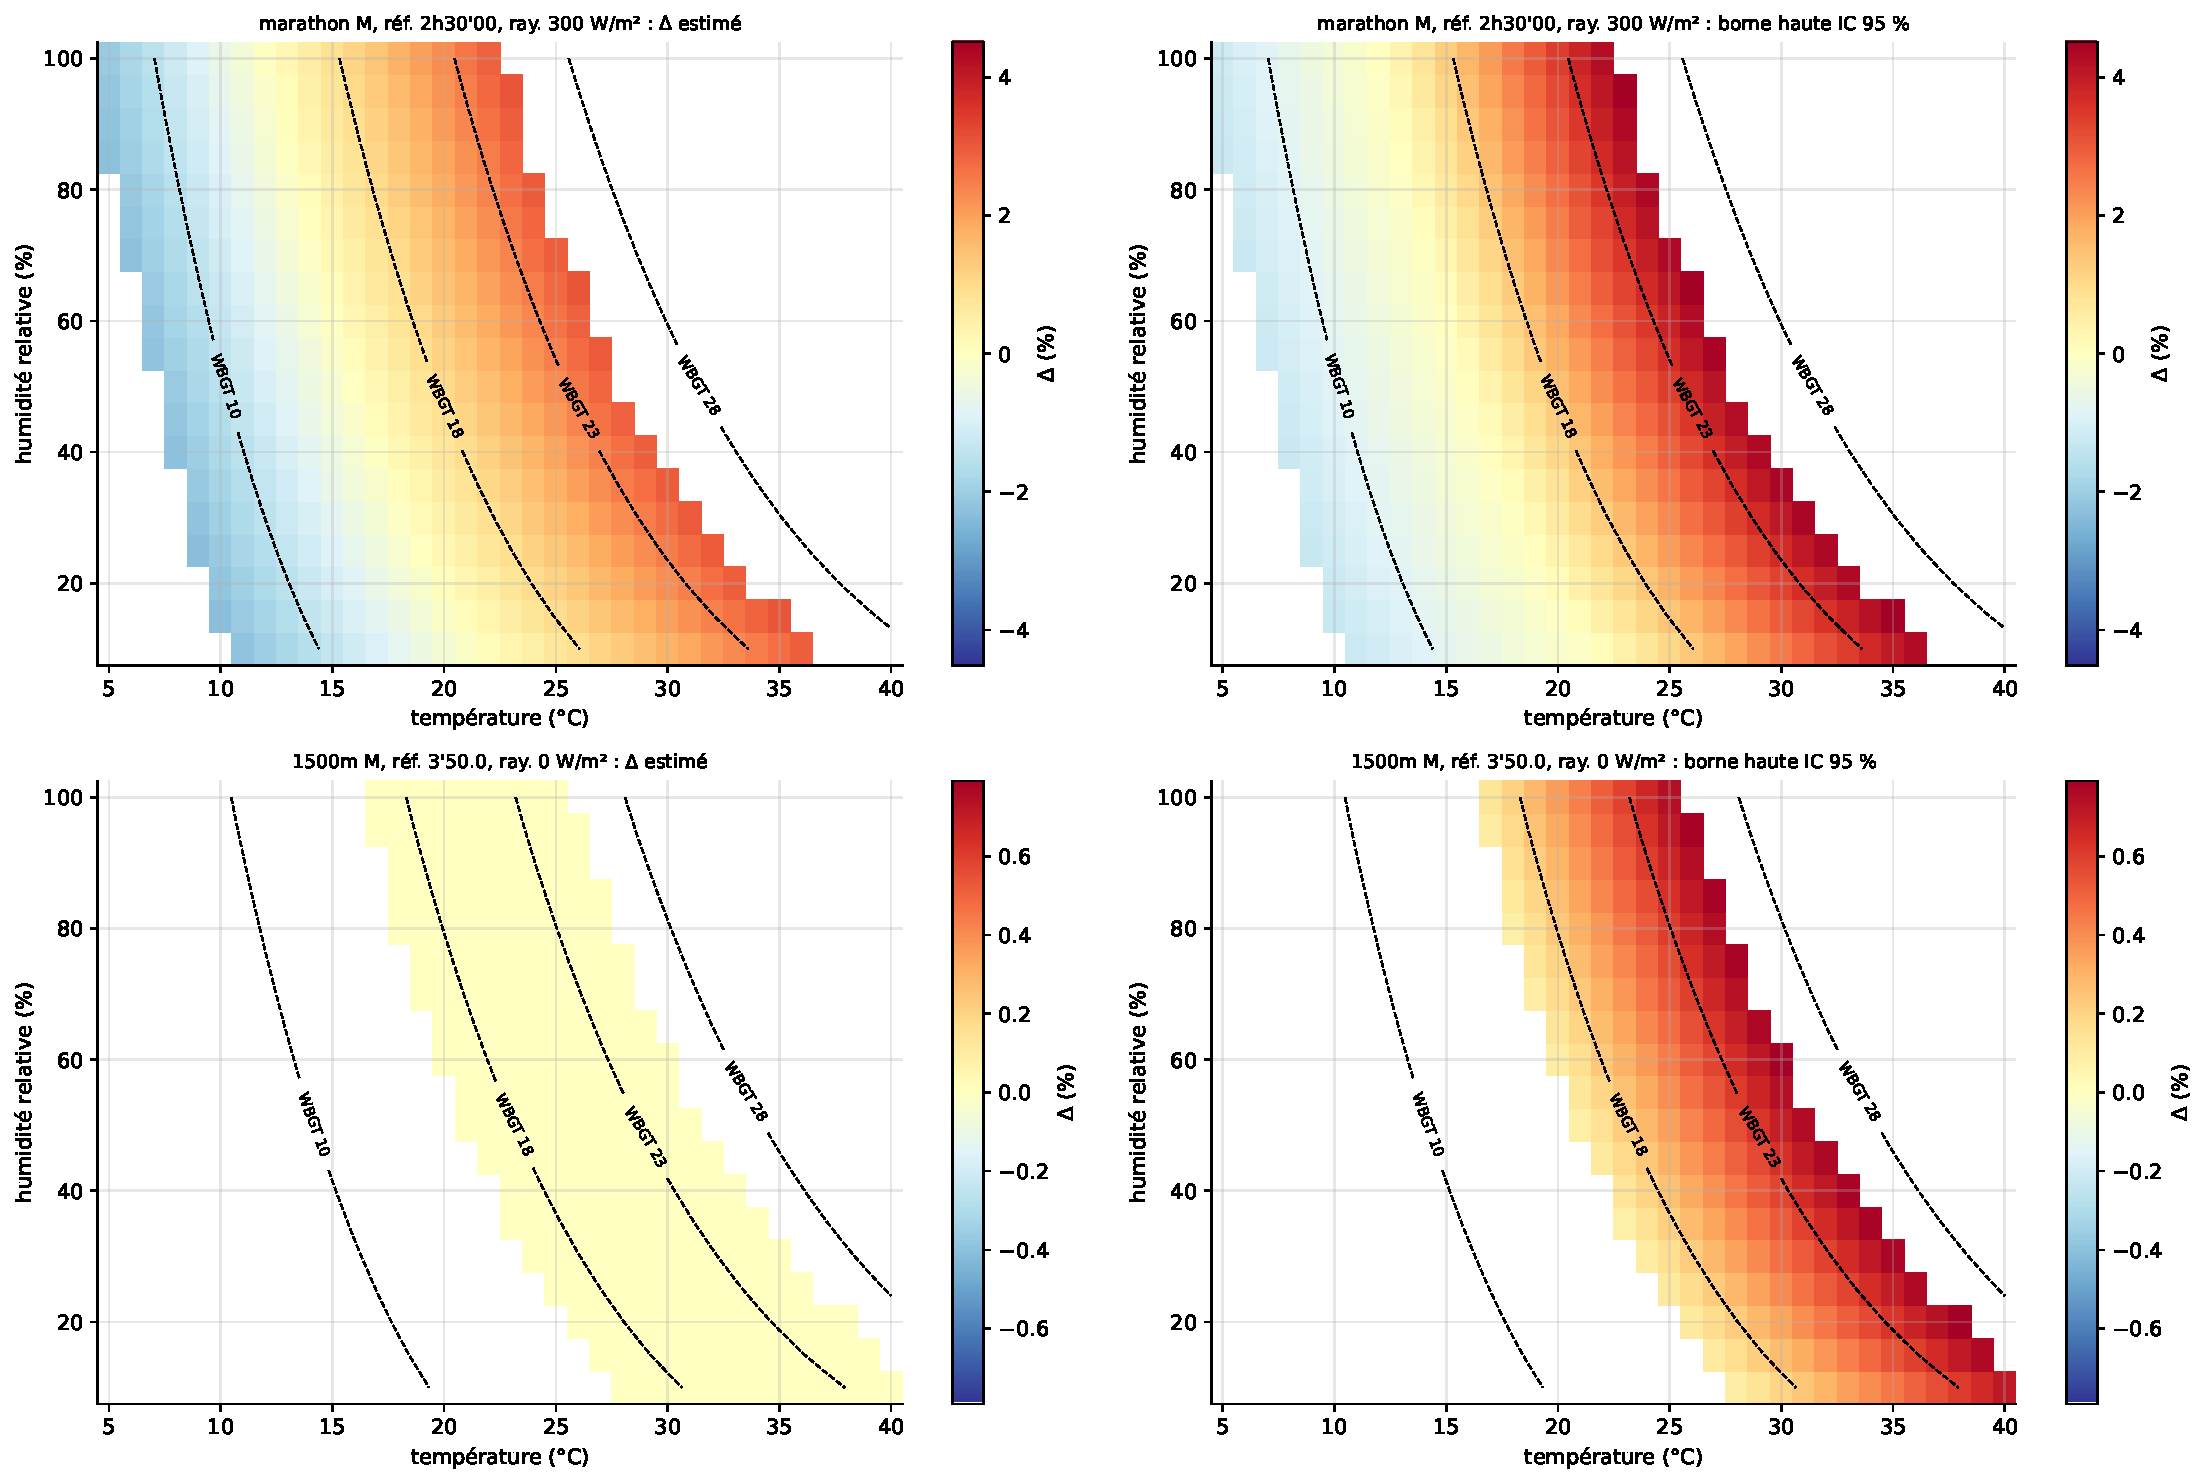
\includegraphics[width=\textwidth]{abaque}
\caption{Abaque de la dégradation $\Delta$ selon la température et l'humidité relative, pour un marathon masculin de
2~h~30 en référence, avec un soleil de 300~W/m² (en haut), et un 1\,500~m masculin de 3~min~50~s, couru en soirée sans
soleil (en bas). À gauche, estimation centrale ; à droite, borne haute de l'intervalle de confiance à 95~\%. Les
isolignes de WBGT 10, 18, 23 et 28~°C correspondent aux seuils de l'ACSM ; les cases blanches sortent de la plage
observée pour le groupe d'épreuves.}
\label{fig:abaque}
\end{figure}

Au marathon, les isolignes de WBGT descendent de gauche à droite : à température égale, l'humidité augmente la charge
thermique, et le soleil ajoute à lui seul plusieurs degrés de WBGT par rapport à l'ombre. La dégradation va de
$-2{,}3$~\% pour un WBGT de 8 à 10~°C, où l'on court plus vite qu'en référence, à $+3{,}0$~\% vers 25~°C ; la borne
prudente va de $-1{,}3$ à $+4{,}5$~\%. À 22~°C, 70~\% d'humidité et au soleil, l'outil conseille 2~h~33~min~10~s, soit
environ 3~min~38~s au kilomètre au lieu de 3~min~33~s. Le tableau~\ref{tab:abaque} donne les chronos équivalents pour
quelques combinaisons. Au total, 41~\% des cases sont blanches, en chaleur humide comme en froid sec : l'outil refuse
d'y répondre plutôt que d'extrapoler une droite. Sur 1\,500~m, la dégradation est nulle (moins de 0,01~point en valeur
absolue) sur toute la plage couverte, de 16 à 25,6~°C, et la borne haute reste sous 0,8~\%, moins de deux secondes sur
3~min~50~s. Mais 70~\% de la grille est blanche : nos données ne contiennent pas de réunion de piste fraîche, et l'outil
ne dit rien d'un 1\,500~m par temps frais.

\begin{table}[htbp]
\centering
\small
\caption{Chronos équivalents à un marathon masculin de 2~h~30 en conditions de référence, selon la température et
l'humidité relative, avec un soleil de 300~W/m² et un vent de 2~m/s : estimation centrale, puis chrono prudent (borne
de l'intervalle de confiance à 95~\%). Un tiret signale une combinaison hors de la plage observée.}
\label{tab:abaque}
\begin{tabular}{@{}lccccc@{}}
\toprule
& 10~°C & 15~°C & 20~°C & 25~°C & 30~°C \\
\midrule
HR 30~\% & 2\,h\,27'03 / 2\,h\,28'20 & 2\,h\,28'48 / 2\,h\,29'20 & 2\,h\,30'34 / 2\,h\,30'51 & 2\,h\,32'21 / 2\,h\,33'30 & 2\,h\,34'09 / 2\,h\,36'11 \\
HR 50~\% & 2\,h\,27'40 / 2\,h\,28'41 & 2\,h\,29'34 / 2\,h\,29'45 & 2\,h\,31'30 / 2\,h\,32'14 & 2\,h\,33'27 / 2\,h\,35'09 & -- \\
HR 70~\% & 2\,h\,28'14 / 2\,h\,29'00 & 2\,h\,30'16 / 2\,h\,30'24 & 2\,h\,32'20 / 2\,h\,33'28 & 2\,h\,34'27 / 2\,h\,36'38 & -- \\
HR 90~\% & 2\,h\,28'46 / 2\,h\,29'18 & 2\,h\,30'55 / 2\,h\,31'21 & 2\,h\,33'06 / 2\,h\,34'37 & -- & -- \\
\bottomrule
\end{tabular}
\end{table}

Le conseil d'allure qui en découle est simple. Sur 1\,500~m, aucun ajustement n'est justifié. Au marathon, il faut
ralentir de 1 à 1,5~\% par tranche de 5~°C de WBGT au-dessus de 15~°C, et viser la borne prudente si l'on ne connaît
pas sa tolérance à la chaleur. Ces chiffres sont des moyennes pour des coureurs de bon niveau, acclimatés ou non, sans
distinction ; la tolérance individuelle, l'acclimatation et l'hydratation peuvent peser beaucoup plus. Au-delà de
23~°C de WBGT, seuil du drapeau rouge de l'ACSM, l'enjeu devient la sécurité plus que le chrono.

\section{Discussion}\label{sec:discussion}

\subsection{La troncature, revisitée avec le modèle final}\label{sec:sensibilite}

L'exploration avait montré que la troncature des listes atténue la pente brute de la chaleur, et nous avions retenu
une marge minimale de 5~\% comme compromis. Restait à vérifier que nos conclusions n'en dépendent pas. Nous avons
réestimé le modèle de l'outil pour plusieurs marges minimales $M$, sur les performances valides de marge au moins égale
à $M$, et calculé dans chaque groupe d'épreuves l'effet d'une hausse du WBGT de 15 à 25~°C (tableau~\ref{tab:marges}).
Si la troncature atténue l'effet de la chaleur, cet effet doit augmenter avec $M$.

\begin{table}[htbp]
\centering
\small
\caption{Effet d'une hausse du WBGT de 15 à 25~°C, en points de $y$, estimé par le modèle de l'outil selon la marge
de troncature minimale $M$ exigée.}
\label{tab:marges}
\begin{tabular}{@{}rrccccc@{}}
\toprule
$M$ & Performances & Demi-fond piste & Fond piste & Route courte & Semi-marathon & Marathon \\
\midrule
0~\% & 14\,221 & $-0{,}06$ & 0,50 & 1,08 & 1,74 & 3,36 \\
3~\% & 12\,275 & 0,01 & 0,53 & 1,30 & 1,71 & 3,23 \\
5~\% & 10\,398 & 0,04 & 0,82 & 1,52 & 1,78 & 3,14 \\
8~\% & 7\,637 & $-0{,}02$ & 0,79 & 1,62 & 1,88 & 3,16 \\
12~\% & 4\,514 & $-0{,}34$ & 1,86 & 1,72 & 1,44 & 3,02 \\
\bottomrule
\end{tabular}
\end{table}

L'effet de la troncature est borné. Au marathon, l'effet reste entre 3,0 et 3,4~points quand $M$ varie de 0 à 12~\% :
le résultat principal est robuste au choix de la marge. Sur route courte, il passe de 1,1 à 1,7~point quand $M$
augmente, dans le sens d'une atténuation par la troncature. Le demi-fond reste proche de 0 quel que soit $M$. Les
valeurs à $M = 12$~\% reposent sur des échantillons réduits de moitié, et le fond sur piste y devient instable. Au
marathon, l'effet diminue même légèrement quand $M$ augmente, à l'inverse de la pente brute : une fois les contrôles
introduits, la troncature n'y biaise plus l'effet de façon détectable, et ces écarts restent dans la marge
d'incertitude des estimations.

\subsection{Validité de la cible}\label{sec:validite_cible}

La cible $y = 100\ln(t/t^{\RP})$ suppose un effort maximal et un record représentatif du niveau du jour. Le record
peut être ancien : $y$ croît fortement avec l'âge, et l'âge, la forme et le niveau ne corrigent qu'en moyenne. Nos
données ne suivent pas les athlètes, si bien que la comparaison se fait entre coureurs semblables, et non chez un même
coureur ; un plan intra-athlète, observant le même coureur dans des conditions différentes, serait plus convaincant.
Enfin, les 6\,222 performances sans record publié, débutants sur la distance ou données manquantes, ont été exclues :
l'échantillon surreprésente les coureurs expérimentés.

\subsection{Les biais possibles et leur sens}\label{sec:biais}

Plusieurs biais subsistent, et la plupart tirent l'effet estimé vers zéro. L'erreur de mesure de la météo en est le
premier. Notre météo vient d'une réanalyse de 9 à 30~km de résolution, sans microclimat (îlot de chaleur urbain,
tribunes) ; sur piste, l'heure est celle du début de la réunion et non de la course. Si l'on observe
$W^{\text{obs}} = W + \epsilon_W$ au lieu du vrai WBGT $W$, avec une erreur $\epsilon_W$ indépendante de $W$ et de
$y$, alors $\Cov(W^{\text{obs}}, y) = \beta_W \Var(W)$ et $\Var(W^{\text{obs}}) = \Var(W) + \Var(\epsilon_W)$, si
bien que la pente estimée tend vers
\[
\beta_W\,\frac{\Var(W)}{\Var(W) + \Var(\epsilon_W)} < \beta_W .
\]
C'est le \emph{biais d'atténuation} : une erreur de mesure aléatoire tire toujours l'effet vers zéro, et d'autant plus
que la variation utile du WBGT est faible, ce qui est le cas de la variation intra-parcours. La sélection
sous-estime aussi l'effet : par forte chaleur, les abandons ne sont pas listés, et certains coureurs renoncent ou
gèrent leur course. L'effet est alors sous-estimé pour le chrono maximal, mais c'est en partie ce qu'un coureur veut
savoir : de combien ralentir pour finir.

La confusion entre lieux reste possible. La chaleur est surtout observée entre lieux, avec un écart-type
intra-parcours d'environ 1~°C seulement, et le pays, le plateau et le profil des parcours ne sont contrôlés
qu'imparfaitement, même si les effets fixes et le terme de Mundlak concordent avec les effets aléatoires.
L'hétéroscédasticité, ensuite, n'est que contournée : l'écart-type intra-course de $y$ double entre la piste et le
marathon, et le modèle mixte à $\sigma^2$ commun a une vraisemblance bimodale, contournée en fixant $\gamma$ mais pas
corrigée. Les intervalles de prédiction, enfin, dépendent de l'échangeabilité, et un pli de calibration non
représentatif leur fait perdre la couverture garantie.

\subsection{Généralisation et pistes d'amélioration}\label{sec:generalisation}

Nos données couvrent des coureurs de bon niveau, un WBGT de 5 à 28~°C, la piste uniquement entre 13,5 et 26~°C en
soirée, et l'altitude uniquement sur route. Rien ne permet d'extrapoler aux coureurs populaires, plus touchés selon
\citet{ely2007}, aux canicules, aux championnats sous climat tropical ou au demi-fond par temps froid. Pour
l'entraînement à allure sous-maximale, « même effort » renvoie plutôt à la fréquence cardiaque ou à la perception de
l'effort, et l'outil ne s'y transpose pas directement.

Plusieurs pistes permettraient d'aller plus loin. Des listes de résultats complètes, abandons compris, supprimeraient
la troncature, et des identifiants d'athlètes autoriseraient un plan intra-athlète. Les heures réelles de départ, des
stations météorologiques proches et le profil des parcours réduiraient l'erreur de mesure et la confusion entre lieux.
Sur le plan statistique, un modèle mixte hétéroscédastique, avec un $\sigma^2$ propre à chaque groupe d'épreuves,
traiterait la bimodalité à sa source ; des effets aléatoires croisés athlète $\times$ course, ou un modèle bayésien
hiérarchique qui rétrécirait l'effet de la chaleur d'un groupe d'épreuves vers celui des autres, permettraient
d'estimer une courbure commune. Une calibration conforme sur plusieurs plis, ou par groupe d'épreuves, rétablirait la
couverture des intervalles de prédiction. Un modèle conjoint de l'abandon et de la performance traiterait la
sélection, et des données de fréquence cardiaque permettraient de transposer l'outil à l'entraînement.

\section{Conclusion}\label{sec:conclusion}

À effort égal, quand le WBGT passe de 15 à 25~°C, la chaleur ne coûte rien de mesurable sur 800~m et 1\,500~m,
environ 1,5~\% sur 5 et 10~km et environ 3~\% au marathon. Le vent coûte environ 0,2~\% par m/s à WBGT égal, et
l'altitude pèse sur route, avec une grande incertitude. En prédiction, les quatre familles de modèles se valent, et
environ un sixième de la variance des performances est prévisible sur un lieu nouveau ; le reste relève de la forme du
jour.

Le chemin pour y parvenir a sans doute autant d'intérêt que le résultat. Chaque difficulté rencontrée a appelé un outil
précis : la troncature des listes, la loi normale tronquée et une marge minimale ; les facteurs confondants, des
contrôles, des interactions et la décomposition de Mundlak ; la dépendance entre coureurs d'une même course, la
validation croisée par lieux, les moindres carrés généralisés et le bootstrap des lieux ; le désaccord entre des
modèles de précision égale, un modèle interprétable choisi sur des critères physiologiques ; la bimodalité de la
vraisemblance, une covariance de travail ; la sous-couverture des intervalles conformes, l'examen de l'hypothèse
d'échangeabilité. Quatre leçons méthodologiques s'en dégagent : valider par groupes quand les données sont
structurées ; estimer l'incertitude par un bootstrap des mêmes groupes ; distinguer prédire et estimer un effet ; et
préférer un outil qui donne un intervalle honnête et refuse d'extrapoler.

\begin{thebibliography}{99}

\bibitem[Aitken(1935)]{aitken1935}
Aitken A. C. (1935). On least squares and linear combination of observations. \emph{Proceedings of the Royal Society
of Edinburgh} 55, 42--48.

\bibitem[Armstrong et~al.(2007)]{armstrong2007}
Armstrong L. E. et~al. (2007). American College of
Sports Medicine position stand. Exertional heat illness during training and competition. \emph{Medicine \& Science in
Sports \& Exercise} 39(3), 556--572.

\bibitem[Bergstra et~Bengio(2012)]{bergstra2012}
Bergstra J., Bengio Y. (2012). Random search for hyper-parameter optimization. \emph{Journal of Machine Learning
Research} 13, 281--305.

\bibitem[Breiman et~al.(1984)]{breiman1984}
Breiman L., Friedman J., Olshen R., Stone C. (1984). \emph{Classification and Regression Trees}. Wadsworth.

\bibitem[Brent(1973)]{brent1973}
Brent R. P. (1973). \emph{Algorithms for Minimization without Derivatives}. Prentice-Hall.

\bibitem[Chen et~Guestrin(2016)]{chen2016}
Chen T., Guestrin C. (2016). XGBoost: a scalable tree boosting system. \emph{Proceedings of the 22nd ACM SIGKDD
International Conference on Knowledge Discovery and Data Mining}, 785--794.

\bibitem[Cybenko(1989)]{cybenko1989}
Cybenko G. (1989). Approximation by superpositions of a sigmoidal function. \emph{Mathematics of Control, Signals and
Systems} 2(4), 303--314.

\bibitem[Efron(1979)]{efron1979}
Efron B. (1979). Bootstrap methods: another look at the jackknife. \emph{The Annals of Statistics} 7(1), 1--26.

\bibitem[Ely et~al.(2007)]{ely2007}
Ely M. R., Cheuvront S. N., Roberts W. O., Montain S. J. (2007). Impact of weather on marathon-running performance.
\emph{Medicine \& Science in Sports \& Exercise} 39(3), 487--493.

\bibitem[Friedman(2001)]{friedman2001}
Friedman J. H. (2001). Greedy function approximation: a gradient boosting machine. \emph{The Annals of Statistics}
29(5), 1189--1232.

\bibitem[Goldstein et~al.(2015)]{goldstein2015}
Goldstein A., Kapelner A., Bleich J., Pitkin E. (2015). Peeking inside the black box: visualizing statistical learning
with plots of individual conditional expectation. \emph{Journal of Computational and Graphical Statistics} 24(1),
44--65.

\bibitem[Grinsztajn et~al.(2022)]{grinsztajn2022}
Grinsztajn L., Oyallon E., Varoquaux G. (2022). Why do tree-based models still outperform deep learning on typical
tabular data? \emph{Advances in Neural Information Processing Systems 35, Datasets and Benchmarks Track}.

\bibitem[Hastie et~al.(2009)]{hastie2009}
Hastie T., Tibshirani R., Friedman J. (2009). \emph{The Elements of Statistical Learning}, 2\textsuperscript{e}
édition. Springer.

\bibitem[Hersbach et~al.(2020)]{hersbach2020}
Hersbach H. et~al. (2020). The ERA5 global reanalysis. \emph{Quarterly Journal of the Royal Meteorological Society}
146, 1999--2049.

\bibitem[Hornik(1991)]{hornik1991}
Hornik K. (1991). Approximation capabilities of multilayer feedforward networks. \emph{Neural Networks} 4(2),
251--257.

\bibitem[Ke et~al.(2017)]{ke2017}
Ke G., Meng Q., Finley T., Wang T., Chen W., Ma W., Ye Q., Liu T.-Y. (2017). LightGBM: a highly efficient gradient
boosting decision tree. \emph{Advances in Neural Information Processing Systems} 30.

\bibitem[Kingma et~Ba(2015)]{kingma2015}
Kingma D. P., Ba J. (2015). Adam: a method for stochastic optimization. \emph{International Conference on Learning
Representations}.

\bibitem[Kish(1965)]{kish1965}
Kish L. (1965). \emph{Survey Sampling}. Wiley.

\bibitem[Koenker et~Bassett(1978)]{koenker1978}
Koenker R., Bassett G. (1978). Regression quantiles. \emph{Econometrica} 46(1), 33--50.

\bibitem[Leshno et~al.(1993)]{leshno1993}
Leshno M., Lin V. Y., Pinkus A., Schocken S. (1993). Multilayer feedforward networks with a nonpolynomial activation
function can approximate any function. \emph{Neural Networks} 6(6), 861--867.

\bibitem[Liang et~Zeger(1986)]{liang1986}
Liang K.-Y., Zeger S. L. (1986). Longitudinal data analysis using generalized linear models. \emph{Biometrika} 73(1),
13--22.

\bibitem[Liljegren et~al.(2008)]{liljegren2008}
Liljegren J. C., Carhart R. A., Lawday P., Tschopp S., Sharp R. (2008). Modeling the wet bulb globe temperature using
standard meteorological measurements. \emph{Journal of Occupational and Environmental Hygiene} 5(10), 645--655.

\bibitem[Lorenzo et~al.(2010)]{lorenzo2010}
Lorenzo S., Halliwill J. R., Sawka M. N., Minson C. T. (2010). Heat acclimation improves exercise performance.
\emph{Journal of Applied Physiology} 109(4), 1140--1147.

\bibitem[Loshchilov et~Hutter(2019)]{loshchilov2019}
Loshchilov I., Hutter F. (2019). Decoupled weight decay regularization. \emph{International Conference on Learning
Representations}.

\bibitem[Lundberg et~Lee(2017)]{lundberg2017}
Lundberg S. M., Lee S.-I. (2017). A unified approach to interpreting model predictions. \emph{Advances in Neural
Information Processing Systems} 30.

\bibitem[Lundberg et~al.(2020)]{lundberg2020}
Lundberg S. M., Erion G., Chen H., DeGrave A., Prutkin J. M., Nair B., Katz R., Himmelfarb J., Bansal N., Lee S.-I.
(2020). From local explanations to global understanding with explainable AI for trees. \emph{Nature Machine
Intelligence} 2(1), 56--67.

\bibitem[Mantzios et~al.(2022)]{mantzios2022}
Mantzios K. et~al. (2022).
Effects of weather parameters on endurance running performance: discipline-specific analysis of 1258 races.
\emph{Medicine \& Science in Sports \& Exercise} 54(1), 153--161.

\bibitem[Mundlak(1978)]{mundlak1978}
Mundlak Y. (1978). On the pooling of time series and cross section data. \emph{Econometrica} 46(1), 69--85.

\bibitem[Patterson et~Thompson(1971)]{patterson1971}
Patterson H. D., Thompson R. (1971). Recovery of inter-block information when block sizes are unequal.
\emph{Biometrika} 58(3), 545--554.

\bibitem[Racinais et~al.(2015)]{racinais2015}
Racinais S. et~al. (2015). Consensus recommendations on training and competing in the heat. \emph{British Journal of
Sports Medicine} 49(18), 1164--1173.

\bibitem[Romano et~al.(2019)]{romano2019}
Romano Y., Patterson E., Candès E. (2019). Conformalized quantile regression. \emph{Advances in Neural Information
Processing Systems} 32.

\bibitem[Rønnestad et~al.(2022)]{ronnestad2022}
Rønnestad B. R. et~al. (2022). Heat suit training increases hemoglobin mass in elite cross-country skiers.
\emph{Scandinavian Journal of Medicine \& Science in Sports} 32(7), 1089--1098.

\bibitem[Shapley(1953)]{shapley1953}
Shapley L. S. (1953). A value for n-person games. In \emph{Contributions to the Theory of Games}, vol. II, 307--317.
Princeton University Press.

\bibitem[Srivastava et~al.(2014)]{srivastava2014}
Srivastava N., Hinton G., Krizhevsky A., Sutskever I., Salakhutdinov R. (2014). Dropout: a simple way to prevent
neural networks from overfitting. \emph{Journal of Machine Learning Research} 15, 1929--1958.

\bibitem[Telgarsky(2016)]{telgarsky2016}
Telgarsky M. (2016). Benefits of depth in neural networks. \emph{Conference on Learning Theory}, 1517--1539.

\bibitem[Vovk et~al.(2005)]{vovk2005}
Vovk V., Gammerman A., Shafer G. (2005). \emph{Algorithmic Learning in a Random World}. Springer.

\bibitem[Zippenfenig(2023)]{zippenfenig2023}
Zippenfenig P. (2023). Open-Meteo.com Weather API. Zenodo, doi:10.5281/zenodo.7970649.

\end{thebibliography}

\end{document}
